%\documentclass[12pt,a4paper,singleside,openright]{toptesi}
\documentclass[12pt,a4paper,cucitura]{toptesi}

\usepackage[utf8]{inputenc}
\usepackage[english]{babel}
\usepackage{subfig}
\usepackage{float}
\usepackage{listings}
\usepackage{longtable}
\usepackage{multirow}
\usepackage{amsmath}
\usepackage{ulem}
\usepackage[pdftex,
pdfauthor={Gianluca Borello},
pdftitle={Statistical Models for Network Anomaly Detection},
pdfsubject={Tesi di Laurea Specialistica},
pdfkeywords={<rdf:li>LaTeX</rdf:li><rdf:li>Tesi</rdf:li><rdf:li>PDF/A</rdf:li>},
pdfa
]{hyperref}
\usepackage{hypcap}

\restylefloat{figure}

\facolta[III]{Ingegneria dell'Informazione}
\corsodilaurea{Ingegneria Informatica}
\titolo{Statistical Models for Network Anomaly Detection}
\logosede{logopolito}
\candidato{Gianluca~Borello}
\relatore{prof.~Fulvio~Risso}
\sedutadilaurea{Novembre 2010}

\graphicspath{{images/}}

%%% comandi comuni
% stampa una pagina completamente vuota
\newcommand*\paginavuota{\clearpage\thispagestyle{empty}\null\clearpage}
% stampa una pagina bianca (solo il numero di pagina)
\newcommand*\paginabianca{\clearpage\null\clearpage}

\begin{document}
\normalem

\frontespizio

\english

\sommario

The term \emph{Anomaly Detection} refers to the problem of finding patterns in a data set that significantly deviate from the characteristics of 
all the other elements of the collection.
This kind of analysis has a huge variety of applications in the real world, including computer networks.
In this thesis, the so called \emph{Network Anomaly Detection} is studied.
There are many approaches in literature to deal with this problem, but most of them are based on rather simple network metrics that are acquired through some popular standards for collecting statistics.
In our approach, we try to see how the clustering analysis technique (chosen because of its popularity and simplicity) behaves when used in combination with more complex (from a semantically point of view) data.

The document starts with a formal definition of \emph{anomaly detection} and \emph{network anomaly detection} (Chapter 1), followed by a short survey of the most popular approaches that are usually considered in the scientific literature (Chapter 2).
Then, the architecture of a clustering-based anomaly detector is proposed, discussed and tested (Chapter 3).
Finally (Chapter 4), on the basis of the considerations and the experience gained during the tests of the previous model, a new and completely invented  model is defined, which is not based on clustering analysis, and attempts to solve some of the biggest problems arising using the combination of clustering algorithms and complex network metrics.

\paginabianca

\indici

\listoffigures
\listoftables
\lstlistoflistings

\chapter{Introduction}
\section{Anomaly detection: definition and applications}

\emph{Anomaly detection} refers to the problem of finding patterns in data that do not conform to expected behavior.
These non conforming patterns are often referred to as \emph{anomalies}, \emph{outliers}, \emph{discordant observations}, \emph{exceptions}, \emph{aberrations}, \emph{surprises}, \emph{peculiarities} or \emph{contaminants} in different application domains.

From a more practical point of view, anomaly detection can be described as a system that triggers an alarm whenever a strange system behavior happens. The concept is closely related to the process of building an \emph{activity profile} of normal usage of a system over an interval of time.
Once in place, the profile is compared against real-time events.
Anything that deviates from the \emph{baseline}, or the norm, is logged as anomalous.

Given the generality and the power of the approach, anomaly detection is applicable in a variety of domains, such as:

\begin{itemize}

\item \textbf{Intrusion detection}: detection of malicious activity (under any form of computer abuse) in a computer related system. These malicious activities or intrusions are interesting from a computer security
perspective.
An intrusion is different from the normal behavior of the system, and hence anomaly detection techniques are applicable in this field.
Intrusions can be classified as \emph{host-based} intrusions (malicious programs, unauthorized behavior, policy violations, etc.) and \emph{network intrusions} (e.g. attacks launched by outside hackers who want to gain unauthorized access to the network, etc.);

\item \textbf{Fraud detection}: detection of criminal activities occurring in commercial organizations such as banks, credit card companies, insurance agencies, cell phone companies, stock market, etc. 
The fraud occurs when there is a consumption of the resources provided by the organization in an unauthorized way, and the organizations are interested in an immediate detection of such frauds to prevent economic losses;

\item \textbf{Image Processing}: detection of any changes in an image over time (motion detection) or in regions which appear abnormal on the image. This domain includes satellite imagery, digit recognition, mammographic image analysis, video surveillance, etc. 
The anomalies are caused by motion or insertion of foreign object or instrumentation errors;

\item \textbf{Medical anomaly detection}: detection of anomalies in patient records.
The data can have anomalies due to several reasons such as abnormal patient condition or instrumentation errors or recording errors.
Anomaly detection in this domain is a very critical problem and requires high degree of accuracy;

\item \textbf{Industrial Damage Detection}: Industrial units suffer damage due to continuous usage and the normal wear and tear.
Such damages need to be detected early to prevent further escalation and losses;

\end{itemize}

\section{Network Anomalies}

This document is focused on \emph{network anomaly detection}.
There are many facets and types of anomalies related to this area, and in literature there are numerous case studies.
In general, the following chapters will not detail any of them, because what we want to do is to build an anomaly detector as \emph{generic} as possible, which is able to detect any abnormal behavior occurring in a network, starting from a time series of network metrics provided as input to the model.
In general, to give an idea of what is the expected output of an anomaly detector operating on a computer network environment, we can identify the following macro categories of alerts:

\begin{itemize}
\item Unusually \emph{peak} of traffic;
\item Traffic \emph{drop};
\item Day not abiding to ``normal'' \emph{weekly pattern};
\item Traffic focused on \emph{certain parts} of the networks, hosts or ports;
\item New application generating \emph{different traffic patterns};
\end{itemize}

\section{``Network Anomaly Detection System'' vs ``Network Intrusion Detection System''}
Although \emph{Network Anomaly Detection System} (\emph{NADS}) and \emph{Network Intrusion Detection System} (\emph{NIDS}) are two technologies often competing, it is worth to spend a few words to clarify the differences between these categories of technologies.

It is quite easy to compare the two approaches: first of all, they both look for ``bad things'' happening on a network, things that may be potential security incidents.
Each can work well or produce loads of false alarms.
And the final results are pretty the same: a suspicious event is flagged for an administrator to investigate.
However, despite these similarities, the two models work quite differently: a \emph{NIDS} uses a defined set of rules or filters that have been written and engineered (almost always manually) to catch a specific, malicious event.
This is often referred to as \emph{misuse} detection.
A \emph{NADS}, on the other hand, operates only from a baseline of normal activity.
As described above, behavior that varies from this standard is detected.
So the difference is that, while an \emph{NIDS} looks for a misuse signature \footnote{The concept of signature has different meanings depending on the context in which the system is used (e.g. a regular expression, a rule to compare with the flow of packets, etc.)}, the \emph{NADS} looks for a strange event.

With these differences in mind, consider the benefits of an \emph{NADS}.
A \emph{NIDS} can only catch events that it has been told to look for.
Anything outside of this list will not be recognized. A \emph{NADS}, in turn, has the potential to detect new, unknown, or unlisted events.
As one can see, it is a very powerful tool.
But how does it determine what is normal? What makes an activity strange? The answer to these questions, and the key to an effective \emph{NADS}, is the \emph{profile} or \emph{baseline}.

For a practical example, consider the typical problem of a \emph{worm}: in order to detect and stop \emph{worms} and \emph{malware}, the system needs to know the existence of a specific kind of threat.
In today's rapidly evolving networks, where attackers are often one step ahead of the products designed to prevent damages, anomaly detection is an important innovation. 
Many vendors rely on signature detection to find network threats.
Customers often have to wait days to get a working signature to insert in their {NIDS} for a new worm, leaving their networks vulnerable in the most critical period during a worm's release.
Instead, by applying anomaly algorithms, anomaly detection can identify \emph{zero-day worms}, \emph{malware}, acceptable-use policy violations and insider misuse. 

Because anomaly detection looks for substantial changes in network behavior, it is less prone to false positives, and requires less configuration and ongoing maintenance than many other security methods.
So network anomaly detection is a very robust and scalable technology.

However, the biggest disadvantage of this technology is that, unlike other methodologies, the underlying principle on which it is based is that anomalies must be significantly different from normal network traffic, and therefore it is virtually impossible to detect certain types of unwanted behaviors whose pattern is similar to the normal one, while for an \emph{NIDS} this is an absolutely trivial task (because in that case only the correct signature for that type of anomaly is needed).

\chapter{Network anomaly detection: state of the art}
\section {Main theoretical approaches}
This section lists the major techniques which can be found in literature regarding network anomaly detection.
Please note that the true list would be much longer, and the points below are not exhaustive (a more complete study can be found in \cite{survey}, while other more innovative approaches are listed in \cite{newsurvey}).
This part will introduce the topic by listing some approaches that contain many similarities with the techniques that are presented in the next sections and have been tested under this research.

In general, all these techniques take as input the whole data set plus some other configuration parameter that varies (e.g. a mathematical model to better describe the typical behavior of the dataset or a threshold to tune the algorithm), and the output provided by any anomaly detection algorithm can be:

\begin{itemize}
\item \textbf{Score}: the algorithm assigns a ``score'' to every instance of the data set, and this value is proportional to the anomaly level of the sample.
In this sense, the output is a ranked list of anomalies, and we can choose to either analyze top few anomalies or use a threshold to select only the most severe anomalies;
\item \textbf{Label}: the algorithm simply assigns a label (which usually is ``normal'' or ``anomalous'') to every instance;
\end{itemize}

\subsection{Classification}
Classification is used to learn a model, the so called \emph{classifier}, from a set of labeled data instances and then, classify a test instance into
one of the classes using the learned model.
Following this concept, classification-based anomaly detection techniques operate in two phases.
During the \emph{training phase} a classifier is built, using the available labeled training data.
The \emph{testing phase} classifies a test instance as normal or anomalous using the classifier.
Classification-based anomaly detection techniques operate under the general assumption that is possible to build a classifier from the data set which can distinguish between normal and anomalous classes. 
Of course this is not always possible, since it can be difficult to have a data set already labeled.

A summary of the advantages and disadvantages of this technique is given in Table \ref{tab-classification}.

\begin{table}
\centering
\begin{tabular}{l|p{12cm}}
\hline
\hline
\multirow{2}{*}{Advantages} & Classification can make use of powerful algorithms that can distinguish between instances belonging to different classes. \\
\cline{2-2}
 & The testing phase is usually very fast since each instance of the set needs to be compared against the already computed model. \\ 
\hline
\multirow{2}{*}{Disadvantages} & Classification relies on the availability of accurate labels for various normal classes, which is often not possible, especially when doing anomaly detection. \\
\cline{2-2}
& Classification assigns a label to each test instance. This can also become a disadvantage when a meaningful anomaly score is desired for
the test instances (however some classification techniques obtains a probabilistic score from the output of a classifier) since in some situations the ``simple'' information ``anomalous'' vs ``not anomalous'' might not be enough. \\
\hline
\hline
\end{tabular}
\caption{Classification - advantages and disadvantages}
\label{tab-classification}
\end{table}

\subsection{Nearest neighbor}

These techniques are extremely popular (and easy to implement), and are based on the assumption that normal data instances occur in \emph{dense neighborhoods}, while anomalies occur far from their \emph{closest neighbors}.
Therefore, these algorithms require a distance or similarity measure defined between two data instances. 
This measure can be computed in different ways. 
For continuous attributes, Euclidean distance is one of the most popular choices, while for categorical attributes, simple matching coefficient is often
used (the next chapter covers with more details some of the distance measures for continuous attributes which are used in the proposed approach).
For multivariate data instances instead, distance or similarity is usually computed for each attribute and then combined.
Nearest neighbor-based anomaly detection techniques can be grouped into two categories:

\begin{itemize}
\item \textbf{Distance-based}: they rely on the idea that the anomaly score of a data instance is defined as its distance to its $k^{th}$ nearest neighbor \footnote{The $k^{th}$ nearest neighbor for a point in the data set can be easily determined by computing the list of the distances from the other points in the data set. By sorting in descending order the list, the nearest neighbor is the element at position $k$.} in the data set;
\item \textbf{Density-based}: in this case, the density of the neighborhood of each data instance is estimated, and then an instance that lies in a neighborhood with low density is declared to be anomalous while an instance that lies in a dense neighborhood is declared to be normal;
\end{itemize}

A summary of the advantages and disadvantages of this technique is given in Table \ref{tab-nearest}.

\begin{figure}
\centering
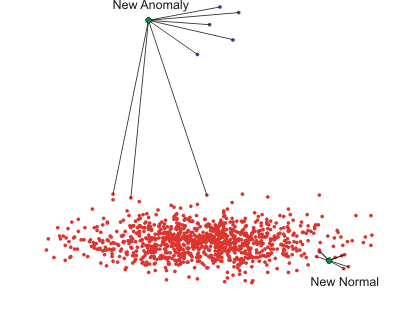
\includegraphics[width=0.5\textwidth]{points.png}
\caption[Nearest neighbor example]{Using a nearest neighbor approach, the data is classified by the average distances to the k closest points.}
\end{figure}

\begin{table}
\centering
\begin{tabular}{l|p{12cm}}
\hline
\hline
\multirow{2}{*}{Advantages} & Nearest neighbor techniques are unsupervised in nature and they do not make any assumptions regarding the distribution of the data. They are purely data driven. \\
\cline{2-2}
& It is really easy to adapt nearest neighbor techniques to a different data type, because the only thing to do is basically define an appropriate distance measure for the given data \footnote{An appropriate measure can be adopted by taking into account various factors such as the dimensionality of the data set, the statistical dependence among the variables, etc.}. \\ 
\hline
\multirow{2}{*}{Disadvantages} & If the data has normal instances that do not have enough close neighbors or if the data has anomalies that have enough close neighbors, these techniques fail to label them correctly, resulting in missed anomalies. \\
\cline{2-2} 
& The computational complexity of the testing phase is a significant challenge since it involves computing the distance of each test instance with all the instances belonging to the test data itself in order to compute the nearest neighbors. \\
\cline{2-2}
& Performance of a nearest neighbor-based techniques greatly rely on the distance measure between pairs of data instances, that can effectively distinguish between normal and anomalous instances, and defining distance measures between instances can be challenging when the data is complex from the point of view of dimensionality, types of values, scales, etc. \\
\hline
\hline
\end{tabular}
\caption{Nearest neighbor - advantages and disadvantages}
\label{tab-nearest}
\end{table}

\subsection{Statistical}

A \emph{statistical} anomaly detection algorithm is based on the assumption that normal data instances occur in high probability regions of a \emph{stochastic} model, while anomalies occur in the low probability regions of the stochastic model.
So, a statistical algorithm tries to fit at a statistical model (usually defined for the normal behavior in the data) to the given data set and then tries to apply a statistical inference test to determine if an unseen instance belongs to this model or not.
Instances that have a low probability to be generated from the expected model, based on the applied test statistic, are declared as anomalies. 
A statistical technique can be parametric, when the knowledge of the underlying distribution for given data is expected, and non-parametric, when the knowledge of the distribution is generally not needed.

As an example, a simple outlier detection technique is to declare all data instances that are more than $3\sigma$ far away from the distribution mean $\mu$, where $\sigma$ is the standard deviation for the distribution. 
The $\mu$ $\pm$ $3\mu$ region contains 99.7\% of the data instances.
This method of course works well only if the data inside the data set can be fitted by a Gaussian distribution.

Another simple technique to detect outliers in a univariate data set under the assumption that the data is generated by a Gaussian distribution, can be obtained by computing the $z$ score for each instance $x$ in the data set (where $\overline{x}$ is the mean and $s$ is the standard deviation of the whole data set):

\begin{center}
\Large
$z = \frac{|x-\overline{x}|}{s}$
\end{center}

To test whether an instance is an outlier or not, we can use this equation:

\begin{center}
\Large
$z > \frac{N - 1}{\sqrt{N}}\sqrt{\frac{t_{\alpha/(2N), N -2}^2}{N-2 + t_{\alpha/(2N), N -2}^2}}$
\end{center}

Here, $N$ is the size of the data set, and $t_{\alpha/(2N), N -2}$ is a value used as a threshold which comes from a $t$-distribution with a significance level of $\alpha/(2N)$.

A summary of the advantages and disadvantages of this technique is given in Table \ref{tab-statistic}.

\begin{table}[h]
\centering
\begin{tabular}{l|p{12cm}}
\hline
\hline
\multirow{2}{*}{Advantages} & If the assumptions regarding the underlying data distribution are true, it is a good solution for anomaly detection. \\
\cline{2-2}
& The anomaly score provided by the algorithm is associated with a confidence interval, which can be used as additional information while making a decision regarding any test instance (e.g. display the ``severity'' of the anomalies found). \\ 
\hline
\multirow{2}{*}{Disadvantages} & It is based on the assumption that the data fits a particular statistical distribution, and this is not always true. \\
\hline
\hline
\end{tabular}
\caption{Statistical - advantages and disadvantages}
\label{tab-statistic}
\end{table}

\subsection{Information theoretic}

These kind of techniques analyze the information content of a data set using different information measures such as \emph{entropy}.
They rely on the assumption that anomalies in data induce irregularities in the information content of the data set.
As an example, if we have a measure to compute the complexity (such as entropy, which a basically a measure about the degree of uncertainty) of the dataset, it is possible to calculate the minimal subset of instances whose complexity is close to the whole set, and the outliers can be identified by the points outside that subset.
In this example, as a measure of the data set's complexity it might be possible to use something like the ``compression ratio'' of the data set.

A summary of the advantages and disadvantages of this technique is given in Table \ref{tab-information}.


\begin{table}
\centering
\begin{tabular}{l|p{12cm}}
\hline
\hline
\multirow{2}{*}{Advantages} & They can operate in an unsupervised mode. \\
\cline{2-2}
& No assumptions are made about the underlying statistical distribution for the data. \\ 
\hline
\multirow{2}{*}{Disadvantages} & The performance and accuracy are highly dependent on the choice of the information theoretic measure. \\
\cline{2-2}
& It is difficult to associate an anomaly score with a test instance. \\
\hline
\hline
\end{tabular}
\caption{Information theoretic - advantages and disadvantages}
\label{tab-information}
\end{table}

\subsection{Spectral}

These algorithms try to find an approximation of the data set using a combination of attributes that capture the bulk of \emph{variability in the data}. 
The basic assumption is that data can be embedded into a lower dimensional subspace in which normal instances and anomalies appear significantly different.
Thus, the approach adopted by spectral anomaly detection techniques is to determine these kind of subspaces in which the anomalous instances can be identified more easily \cite{pca2}.

One of the most famous spectral techniques is \emph{Principal Component Analysis} (\emph{PCA}), for projecting data into a lower dimensional space.
The \emph{PCA} method is analyzed later, because in our approach it is taken under consideration as a pre-processing step for dealing with really high dimensionality data sets.

A summary of the advantages and disadvantages of this technique is given in Table \ref{tab-spectral}.

\begin{table}
\centering
\begin{tabular}{l|p{12cm}}
\hline
\hline
\multirow{2}{*}{Advantages} & They automatically perform dimensionality reduction and hence are suitable for handling high dimensional data sets. Moreover, they can also be used as a pre-processing step followed by application of any existing anomaly detection technique (and this is exactly what we do in the first proposed approach). \\
\cline{2-2}
& They can operate in an unsupervised mode. \\ 
\hline
\multirow{2}{*}{Disadvantages} & They are useful only if the normal and anomalous data are separable in a lower dimensional space. \\
\cline{2-2}
& They typically have high computational complexity. \\
\hline
\hline
\end{tabular}
\caption{Spectral - advantages and disadvantages}
\label{tab-spectral}
\end{table}

\subsection{Clustering}

\subsubsection{Clustering definition}

Since the first proposed approach uses a \emph{clustering} algorithm to detect anomalies (the second one is not based on any popular technique, because it is mainly based on empirical observation), we will say something more about this technique (a detailed survey about the clustering analysis can be found in \cite{datamining}).

Clustering is mainly a technique used to group similar data instances into clusters, and it is primarily an \emph{unsupervised} approach, even if some semi-supervised clustering techniques exist.

It might not be easy to understand the differences with the nearest neighbors approach, since at first sight these two techniques seem to treat the data in a quite manner similar.
Indeed, clustering can be seen as an efficient way to find nearest neighbors: finding neighbors with traditional algorithms usually requires computing the pairwise distance between all points.
But typically, clusters and their cluster centroids can be found much more efficiently, and, since the points are usually close to their cluster centroid, then it is possible to use those centroids instead of the original points, and this way the number of distance computation necessary to find the nearest neighbor of a generic point are heavily reduced.

From a formal point of view, a clustering algorithm works on a data set $X$ consisting of data points $x_i = (x_{i1}, etc., x_{id}) \in A$ in a multi dimensional space $A$, where $i = 1:N$ , and each component $x_{il} \in A_{l}$ is a numerical or nominal categorical.
Such data format conceptually corresponds to a $N \times d$ matrix and is used by the majority of algorithms.
As said before, the goal of clustering is to assign points to a finite system of $k$ subsets, clusters, and their union is equal to the full data set, with possible exception of outliers.

\subsubsection{Clustering and anomaly detection}

By grouping a set of data into subsets so that instances in the same cluster are similar in some sense, it is possible to detect outliers following one of these assumptions:

\begin{itemize}
\item Normal data instances belong to a cluster in the data, while anomalies \emph{do not belong} to any cluster;
\item Normal data instances lie close to their closest cluster centroid (the cluster center), while anomalies are \emph{far away} from their closest cluster centroid;
\item Normal data instances belong to large and dense clusters, while anomalies either belong to \emph{small or sparse} clusters;
\end{itemize}

Even though clustering and anomaly detection appear to be fundamentally different from each other, several clustering-based anomaly detection techniques have been developed, and in our approach we try to detect some network anomalies using some popular clustering algorithms.

A summary of the advantages and disadvantages of this technique is given in Table \ref{tab-cluster}.

\begin{figure}
\centering
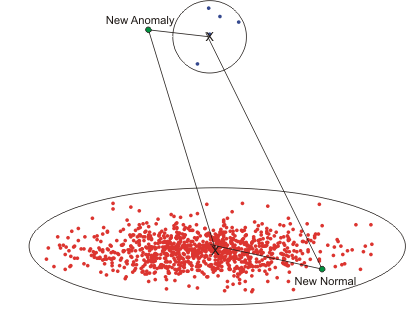
\includegraphics[width=0.5\textwidth]{clusters.png}
\caption[Clustering example]{In clustering analysis, the data is classified by the closest cluster center.}
\end{figure}

\begin{table}
\centering
\begin{tabular}{l|p{12cm}}
\hline
\hline
\multirow{2}{*}{Advantages} & They can operate in an unsupervised mode. \\
\cline{2-2}
& The testing phase is fast since the number of clusters against which every new instance needs to be compared is usually small. \\ 
\hline
\multirow{2}{*}{Disadvantages} & Performance and accuracy are highly dependent on the effectiveness of the algorithm in capturing the cluster structure of normal instances with respect to the anomalies. \\
\cline{2-2}
& There might be some problems when the anomalies form significant clusters among themselves. \\	
\cline{2-2}
& The computational complexity is often a bottleneck. \\
\hline
\hline
\end{tabular}
\caption{Clustering - advantages and disadvantages}
\label{tab-cluster}
\end{table}

\subsubsection{Clustering taxonomy}

A generic clustering algorithm can be classified according to the following taxonomy:

\begin{itemize}
\item \textbf{Hierarchical versus Partitional}: this category distinguishes whether the set of clusters created by the algorithm is nested or unnested, or, in a more traditional terminology, \emph{hierarchical} or \emph{partitional}.
A partitional clustering is simply a division of the set of data objects into non-overlapping clusters such that each data object is in exactly one
of them.
If we permit clusters to have subclusters, then we obtain a hierarchical clustering, which is a set of nested clusters that are organized as a tree.
Each cluster in the tree (except for the leaf nodes) is the union of its children, and the root of the tree is the cluster containing all the objects.
Often, but not always, the leaves of the tree are clusters of individual data objects. Finally, it is possible to note that a hierarchical clustering can be viewed as a sequence of partitional clusterings and a partitional clustering can be obtained by taking any member of that sequence, by cutting the hierarchical tree at a particular level for example.

\begin{figure}
%\centering
\subfloat[Partitional clustering]{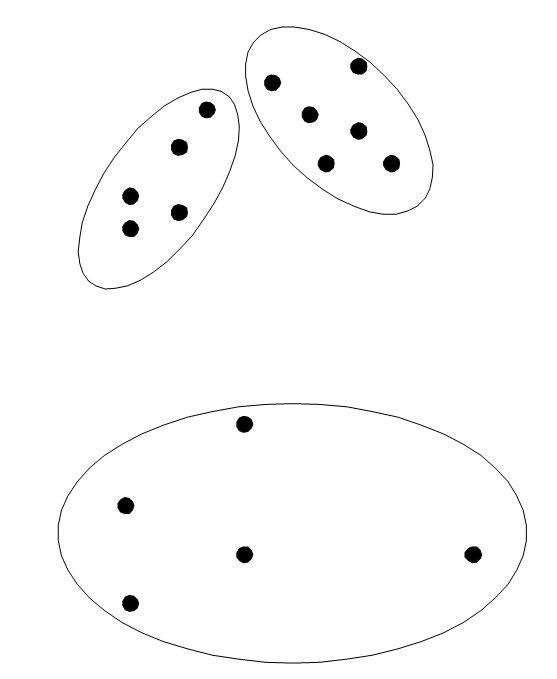
\includegraphics[width=0.5\linewidth, height=5cm]{clusters-partitional.png}}
\subfloat[Hierarchical clustering]{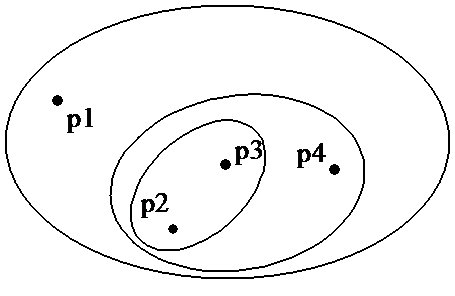
\includegraphics[width=0.5\linewidth, height=5cm]{clusters-hierarchical.png}}
\end{figure}

\item \textbf{Exclusive versus Overlapping versus Fuzzy}: in an \emph{exclusive} clustering, the algorithm assigns each object to a single cluster.
There are many situations in which a point could reasonably be placed in more than one cluster, and these situations are better addressed by non-exclusive clustering.
In the most general sense, an \emph{overlapping} or \emph{non-exclusive} clustering is used to reflect the fact that an object can simultaneously belong to more than one cluster. 
A non-exclusive clustering is then used when an object is between two or more clusters and could reasonably be assigned to any of these clusters.
In a \emph{fuzzy} clustering instead, every object belongs to every cluster with a membership weight that is between 0 (absolutely does not belong) and 1 (absolutely belongs).
In other words, clusters are treated as fuzzy sets (a fuzzy set is one in which an object belongs to any set with a weight that is between 0 and 1). Similarly, probabilistic clustering techniques compute the probability with which each point belongs to each cluster.

\item \textbf{Complete versus Partial}: a \emph{complete} clustering assigns every object to a cluster, whereas a \emph{partial} clustering does not.
The motivation for a partial clustering is that some objects in a data set may not belong to well defined groups.
Many times objects in the data set may represent noise, outliers, or uninteresting background.
In other cases, a complete clustering of the objects is desired.
\end{itemize}

Furthermore, the types of data that can be analyzed during clustering are very heterogeneous, and therefore different types of clusters exist, depending on the nature of the data (e.g. how the points are distributed in the dimensional space). Usually, a specific clustering algorithm finds only a specific type of cluster. It is possible to distinguish between different types of clusters, which can be grouped according to the following taxonomy:

\begin{itemize}
\item \textbf{Well separated}: when a cluster is a set of objects in which each object is closer to every other object in the cluster than to any object not in the cluster.
This idealistic definition of a cluster is satisfied only when the data contains natural clusters that are quite far from each other.
Well separated clusters do not need to be globular, but can have any shape.

\begin{figure}
\centering
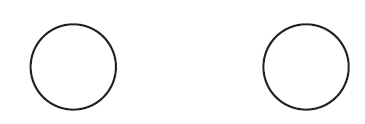
\includegraphics[width=0.5\textwidth]{clusters-well.png}
\caption{Well separated clusters.}
\end{figure}

\item \textbf{Center-based}: when a cluster is a set of objects in which each object is closer to the center that defines the cluster than to the center of any other cluster.
For data with continuous attributes, the center of a cluster is often a centroid, for example the average of all the points in the cluster.
When a centroid is not meaningful, such as when the data has categorical attributes, the center is often a medoid, for example the most representative point of a cluster.

\begin{figure}
\centering
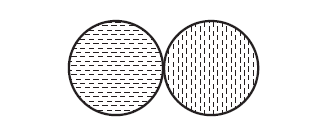
\includegraphics[width=0.5\textwidth]{clusters-center.png}
\caption{Center-based clusters.}
\end{figure}

\item \textbf{Contiguity-based}: when each point in a cluster is closer to some other object in the cluster than to any point in a different cluster.
This definition of a cluster is useful when clusters are irregular or intertwined, but can have trouble when noise is present, since a small bridge of
points can merge two distinct clusters.

\begin{figure}
\centering
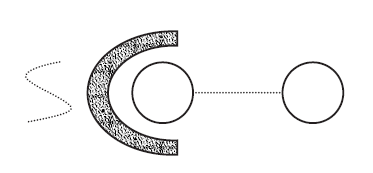
\includegraphics[width=0.5\textwidth]{clusters-contiguity.png}
\caption{Contiguity-based clusters.}
\end{figure}

\item \textbf{Density-based}: when a cluster is a dense region of points that is surrounded by a region of low density. 
A density based definition of a cluster is often employed when the clusters are irregular or intertwined, and when noise and outliers are present.
\end{itemize}

\begin{figure}
\centering
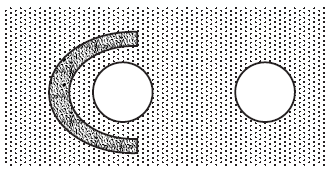
\includegraphics[width=0.5\textwidth]{clusters-density.png}
\caption{Density-based clusters.}
\end{figure}

In literature a lot of clustering algorithms have been proposed, and each technique can be evaluated according to the following properties:

\begin{itemize}
\item Type of \emph{attributes} the algorithm can handle (e.g. numeric or categorical);
\item \emph{Scalability to large data sets};
\item Ability to work with \emph{high dimensional data};
\item Ability to find clusters of \emph{irregular shape};
\item Handling \emph{outliers};
\item \emph{Time complexity} (from a computational point of view);
\item Reliance on a priori knowledge and \emph{user defined parameters};
\item \emph{Interpretability} of results;
\end{itemize}

\chapter{First approach: network anomaly detection using a clustering approach}

In this first proposed approach, the architecture of a network anomaly detector which is able to consider complex metrics is described.
The detector is based on a clustering algorithm, and during the tests we tried two of the most popular ones, \emph{K-Means++} and \emph{DBSCAN}.
At this point, we assume that we have available a capture engine to extract the data we are interested in from different sources of network traffic (e.g. simple traffic traces, data from network sensors placed at strategic points on the network topology, etc.).
A similar engine is available in the product \emph{CACE Pilot}, which was used during the implementation phase (an entire chapter is dedicated to describe the architecture of this product is from a technical point of view).
\emph{Pilot} allowed us to gather a lot of network metrics, and basically mix them together, using the concept of ``traffic view'', in order to capture a lot of interesting informations about the network.

\section{Choosing network metrics: an alternative to NetFlow}

All these informations (the traffic metrics) are exported as \emph{time series}, without doing any particular operation on them (even if the engine is enough complicated by itself, considering the fact that some features we are interested in can be particularly tricky to calculate).
For example, some of the traffic metrics which are quite interesting to observe in order to discover network anomalies are (the list does not pretend to be complete and exhaustive, but it is based on the informations that, from an objective point of view, seem to be more important when analyzing a network \cite{ntop}):

\begin{itemize}
\item \textbf{Bandwidth over time}: The number of bits/bytes/packets per second. It is a good and generic metric since it gives an overview of the traffic amount and its trend;
\item \textbf{Network protocols distribution}: Amount of packets per second for each type of network traffic. This metric gives a great overview of how the network is utilized by the different protocols and applications. It breaks the network traffic into the following categories: \emph{Routing}, \emph{Web}, \emph{Email}, \emph{Data Transfer}, \emph{SSH/Telnet}, \emph{MS Networking}, \emph{SNMP}, \emph{VPN/Tunnel}, \emph{Remote-Desktop}, \emph{VoIP}, \emph{Database}, \emph{IM};
\item \textbf{Number of active hosts over time}: The number of unique active \emph{IP} addresses, i.e. the number of \emph{IP} addresses that either transmit or receive network packets. This metric is very useful, because it is usually not affected by noise \footnote{The concept of noise is widely detailed in the next chapter. In general, a metric is noisy when its typical pattern is hidden by pseudo-random variations, usually due to external factors} and can be used as a snapshot of the network during normal usage condition, to quickly spot anomalous behavior in the future;
\item \textbf{Number of DNS requests over time}: Analysis of the \emph{Domain Name System (DNS)} requests;
\item \textbf{\emph{ICMP} bandwidth over time}: it is well known that the amount of \emph{ICMP} traffic is closely linked to the health status of the network, so it is useful to monitor this metric;
\item \textbf{Local vs non-local traffic}: Comparison between \emph{internal} and \emph{external} traffic for the subnet under observation, in terms of local bandwidth versus the bandwidth with the external world. This can help to discover some strange network activity;
\item \textbf{\emph{IP} bandwidth by country}: The number of bits/bytes/packets per second grouped for the country of each \emph{IP} address;
\item \textbf{Distribution of HTTP status codes}: This metric keeps tracks of the \emph{HTTP} status codes distribution generated on the network. It can be very useful to detect anomalies when the capture engine is set to analyze the traffic on the link between a web server and the Internet. For examples, in most cases, codes \emph{200 (OK)} and \emph{304 (Not Modified)} correspond to the majority of the responses. An abundance of codes \emph{301 (Moved Permanently)} and \emph{302 (Found)} may indicate stale links, while codes \emph{403 (Forbidden)} and \emph{404 (Not Found)} may indicate intrusion attempts or broken links.
Other codes, such as \emph{216 (Partial Content)} and \emph{207 (Multi-Status)} can capture the information about the typical pattern of the users and their applications, such as download accelerators or \emph{PDF} readers. Acceptable values in this metric depend on the type of monitored traffic, but ideally the anomaly detector can create a ``customized'' baseline of every specific network.
\item \textbf{Distribution of \emph{IP TTL}}: This metric gives the trend of the \emph{IP Time to Live} field. This measure can be used to spot unusual network conditions or attacks \footnote{Even if it does not look quite evident, some attacks based on IP TTL exist, like the TTL Expiry flaw \url{http://www.cisco.com/web/about/security/intelligence/ttl-expiry.html}};
\item \textbf{Distribution of the \emph{TCP} receiver window size}: Analysis of the \emph{TCP} window size, for both the \emph{client-server} and the \emph{server-client} directions. The \emph{TCP} window indicates how many bytes a \emph{TCP} endpoint will accept before its reception buffer fills up. It is a good indication of how well a host is coping with the amount of traffic it is receiving. If the window of a host shrink too much, it means that the host is not keeping up with the data rate. When the window reaches zero, the host will effectively stop receiving data, and this is an interesting anomaly to detect;
\item \textbf{Distribution of \emph{TCP} flags}: This metric captures the number of packets transmitted for every combination of \emph{TCP} flags. This measure can be used to spot abnormal network behavior, both short and long term. For example, in a healthy network, the \emph{ACK} and \emph{PSH-ACK} flag combinations should  generate the majority of the \emph{TCP} traffic. Another thing this metric could help to detect is the \emph{SYN} and \emph{SYN-ACK} correspondence: mismatched ratios of \emph{SYN} and \emph{SYN-ACK} might indicate connectivity or configuration problems in the network (or attacks such as port scan);
\item \textbf{Distribution of \emph{TCP} errors}: This metric captures the distribution of the different \emph{TCP} errors over time.
The errors detected are: \emph{retransmissions}, \emph{out of order segments}, \emph{lost segments}, \emph{duplicate ACKs}, \emph{refused connections}, \emph{reset connections} and \emph{zero windows};
\item \textbf{Number of \emph{TCP} errors by traffic type}: Number of \emph{TCP} errors for some different types of application-layer protocols based on \emph{TCP}. The errors detected are: \emph{retransmissions}, \emph{out of order segments}, \emph{lost segments}, \emph{duplicate ACKs}, \emph{refused connections}, \emph{reset connections} and \emph{zero windows};
\item \textbf{Number of \emph{TCP} requests by traffic type}: With this metric we try to capture the chattiness of a specific application. The chattiness of a protocol is the number of \emph{TCP} \emph{client-to-server} requests per second that happen for that protocol. Some protocols, like for example \emph{SSH}, tend to cause a lot of \emph{TCP} packets to go back and forth, which can cause overload of network devices and higher resources consumption.
\item \textbf{Average service response time by traffic type}: Average response times for the major network application types. This metric measures the time between the last client request packet and the first server response packet. If the packet capture happens near the server, it measures the time that a server takes to process a request, and it is one of the best indicators of server performance problems;
\end{itemize}

The reason why we emphasize the term ``complex metrics'' is that this assumption is particularly original, because usually the de facto standard for network anomaly detection is to use the data collected by a protocol such as \emph{NetFlow} \cite{netflow}.
\emph{NetFlow} is a network protocol developed by Cisco Systems to run on network devices for collecting \emph{IP} traffic information.
Devices that have the \emph{NetFlow} feature enabled generate records which are exported to the user using a standardized packet format.
The basic information unit for \emph{NetFlow} is a network flow, which can be seen basically as an unidirectional sequence of \emph{IP} packets all sharing all of the following 7 values:

\begin{itemize}
\item Source \emph{IP} address;
\item Destination \emph{IP} address;
\item Source port for \emph{UDP} or \emph{TCP} flows;
\item Destination port for \emph{UDP} or \emph{TCP} flows;
\item Type and code for \emph{ICMP} flows;
\item \emph{IP} protocol;
\item \emph{IP} Type of Service;
\end{itemize}

Therefore, using a protocol such as \emph{NetFlow}, we can not go further than these metrics, which still represent a considerable part of the information about a network that one generally wants to achieve, but may still be limited (e.g. there are no metrics about performance).

Moreover, maintaining \emph{NetFlow} data can be computationally expensive for a router (99\% of network devices capable to export \emph{NetFlow} traffic are routers), and in order to avoid problems caused by router CPU load, Cisco provides sampled flows.
Basically, rather than looking at every packet to maintain \emph{NetFlow} records, the router looks at every $n$th packet, where $n$ can be configured or it is a randomly selected interval, and, when this approach is used, the records must be adjusted for the effect of sampling.
In this sense, when using sampled flows, metrics are only an estimate rather than the real values, and it is clearly evident the loss of information, especially in limited sized networks such as small and medium businesses, where the typical network pattern is certainly much less stable than in larger scenarios.

\begin{figure}
\centering
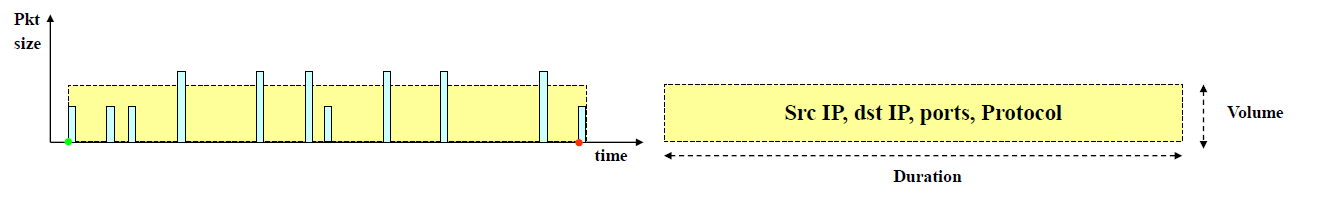
\includegraphics[width=\textwidth]{netflow.png}
\caption[\emph{NetFlow}]{Using \emph{NetFlow}, the concept of packet is lost. All you have is a labeled brick, identified by the flow features, carrying information about its duration and volume.}
\end{figure}

Obviously, for our purposes we can not use an acquisition engine based on \emph{NetFlow}, since our metrics are captured only if we work with a packet-based architecture, analyzing all network traffic without sampling. For this reason, we do not make use of \emph{NetFlow}, and with this assumption we can then build our model around the ideas of ``avoid losing data'' and ``complex metrics''.

\section{Proposed model: schema of the components}

The basic steps of the proposed model are then: 

\begin{enumerate}
\item \textbf{Metrics acquisition}: The capture engine, which is set up to catch the data on a specific section of the network (e.g. the up link connection towards the Internet, the link between a server and the outside world, etc.), captures the information under the form of metrics (such as the ones explained before, but in the typical scenario the user interested in doing anomaly detection can basically create every metric he wants). Each metric can be calculated using the whole traffic crossing the analyzed link, or, alternatively, it is possible to specify a filter to analyze only a subset of traffic (e.g. only one host rather than the full list of hosts transmitting or receiving packets over the monitored link). At regular time intervals, the engine exports the metrics as time series. Basically, it is possible to set any value for the \emph{time aggregation granularity} (typical values can be one second, ten seconds, one minute, thirty minutes, one hour, etc.) but, since the computational cost of clustering algorithms grows more than linearly with the number of data analyzed, a good compromise is obtained by choosing to obtain a new sample for every metric each hour, or each day. The second proposed approach, easier from a computational point of view, completely removes this constraint, and is more appropriate if the goal is having a more reactive anomaly detector;
\item \textbf{Preprocessing}: Suppose we have configured the engine to catch ten network metrics, with a time aggregation interval of one hour. Then, every hour the engine will export ten new samples, containing the updated values for the previous hour. At this step, these values are aggregated into a matrix of $M \times N$, where $M$ is the number of available samples for each metric (e.g. if we consider a total period of six months, the number of samples will be equal to about $6 \times 30 \times 24 = 4320$), and $N$ is the number of metrics. This matrix represents the multi-dimensional space on which the clustering algorithm will work, and when it becomes extremely large, the clustering algorithms have several problems (especially when increasing the number of metrics, rather than the number of points). This problem, widely explained in the next section, is partially solved at this stage, doing a sort of ``reduction'' of the matrix, eliminating, if necessary, the less important informations from a statistical point of view;
\item \textbf{Normalization}: At this point, the multi-dimensional space is almost ready to be analyzed, but a pretty simple step is still needed. As described in the next section, it is necessary to define a suitable distance measure to capture the ``proximity'', or ``similarity'',  information of a point with respect to another point in the space. Since many of the metrics are completely different each other in terms of magnitude and type of numeric values, in this step, if necessary, a data normalization based on the statistical properties of the samples is done;
\item \textbf{Clustering engine}: This is obviously the main step. The matrix containing the data, reduced and normalized if necessary, is given as input to the clustering algorithm, which attempts to create a ``baseline'' of the network metrics by grouping the points in clusters, representing the most frequently patterns. Depending on the used algorithm, after the clusters are determined, it is possible to detect the presence of outliers. For example, using a density-based clustering algorithm, the outliers are all the points that have not formed any cluster, while using other algorithms, outliers can be identified as the points of a cluster which are very far from their respective centroid, or as the points belonging to a cluster smaller than a specific threshold;
\item \textbf{Model update}: Since the clustering step can be particularly long from a computational point of view (especially when the available data is really large), we can basically choose between two methods for updating the model:
\begin{itemize}
\item \textbf{Online update}: Every time the capture engine returns a new set of values, an instance of the clustering algorithm is executed. Of course this method produces the better results, but realistically it might be impossible to use it in certain cases, especially when the time aggregation interval is small;
\item \textbf{Offline update}: in this second scenario, the model is updated only occasionally (e.g. on a weekly basis), and every time new metrics are collected, the new points are compared with the already constructed model (e.g. the coordinates and the size of the clusters from the last run are stored in memory, and a check is done to see if the new points can fit an existing cluster or not).
\end{itemize}
\end{enumerate}

In the following sections each point will be analyzed with more details from a formal point of view.

\begin{figure}
\centering
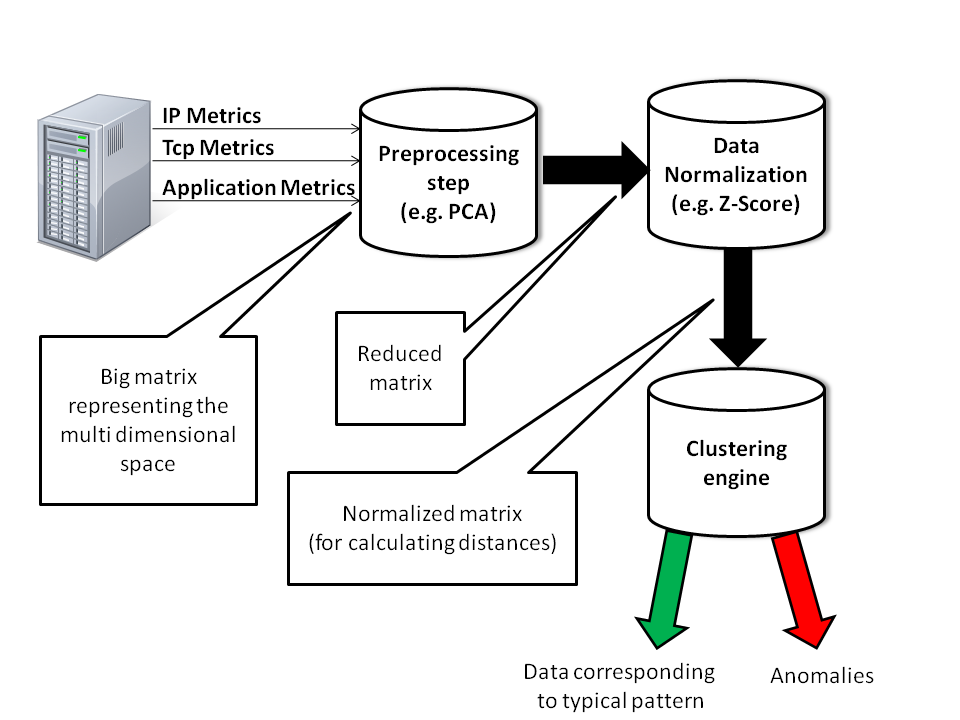
\includegraphics[width=\textwidth]{clustering-architecture.png}
\caption[Clustering-based anomaly detector model]{General architecture of the clustering-based network anomaly detector.}
\end{figure}

\section{Preprocessing: dimensionality reduction using Principal Component Analysis}
\subsection{Dealing with curse of dimensionality}
One of the biggest problems (perhaps the greatest) that occur when dealing with data from the real world which contains a lot of attributes (or dimensions) is the so called \emph{curse of dimensionality}.
This problem is caused by the exponential increase in volume associated with adding extra dimensions to a multi dimensional space.
For example, 100 evenly-spaced sample points suffice to sample a unit interval with no more than 0.01 distance between points; an equivalent sampling of a 10-dimensional unit hypercube with a lattice with a spacing of 0.01 between adjacent points would require 10$^{20}$ sample points: thus, in some sense, the 10-dimensional hypercube can be said to be a factor of 10$^{18}$ ``larger'' than the unit interval.
This problem is really annoying, since the the data set could have hundreds of attributes.
Clustering in such high dimensional spaces presents tremendous difficulty, because the presence of irrelevant dimensions (e.g. the attributes which are basically constant) eliminates any hope on clustering tendency, and the likelihood of presence and number of irrelevant attributes grows with the dimensions.
Moreover, in high dimensional space the distance to the nearest neighbor becomes indistinguishable from the distance to the majority of points, and this effect starts to be severe for dimensions greater than 15. 

\begin{figure}
\centering
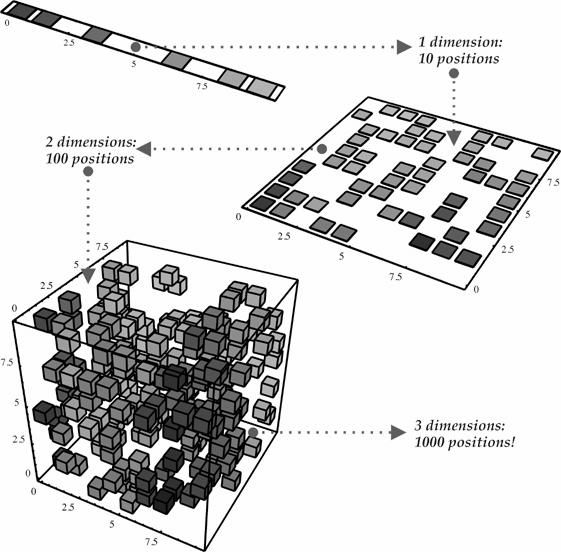
\includegraphics[width=0.5\textwidth]{CurseDimensionality.jpg}
\caption[Curse of dimensionality]{A graphic visualization of the curse of dimensionality problem. In high dimension, the neighborhood becomes exponentially large, and one requires an exponential number of samples to cover it. To cover and discriminate among N regions in the space, one would need $O(N)$ samples, but $N$ can grow to the power for the space dimension.}
\end{figure}

This issue is absolutely present in the field of network anomaly detection, at least in the approach that was followed during this research. In particular:

\begin{itemize}
\item We use a clustering algorithm for the tests, and it's well known that the results of a clustering engine heavily depend on the way the distance between the points is computed. If we have a space with many dimensions, the distance measurement quickly becomes less meaningful, and so the whole output produced by the system tends to be in such a way ``random''.
\item As already mentioned, one of the most original features of this research is the use of detailed network analysis as input to the anomaly detection system, which is not usually done by the other engines based on protocols like Cisco \emph{NetFlow}. Consequently, very often the data analyzed is composed by multivariate time series with very high dimensionality (e.g. distribution of the major network protocols which are being transmitted over the network, distribution of various kinds of  errors, application-level features, etc.), and so we must take extra care to this problem in order to avoid getting the measures meaningless.
\end{itemize}

Therefore, we investigated the major solutions which can be found in literature to solve this problem, and after several tests we have chosen the one that was particularly effective and not expensive from a computational point of view. This technique is called \emph{Principal Component Analysis (PCA)}, and will be briefly illustrated with an example which can help to understand how it can be used to ``reduce'' a high-dimensional space.

So, assuming that problems arise when performing recognition in a high dimensional space (this happened during the first tests on a real scenario), significant improvements can be achieved by first mapping the data into a lower-dimensionality space, and basically the goal of \emph{PCA} is to reduce the dimensionality of the data while retaining as
much as possible of the variation present in the original data set.
This result is achieved by computing a linear transformation that maps data from a high dimensional space to a lower dimensional space.

\subsection{An example}
This section covers the steps needed to perform \emph{PCA} on a set of data. 
An explanation of what is happening at each point is provided, so that it will be easy to understand why this technique works.

\begin{enumerate}
\item \textbf{Get some data}: In this simple example, we use a real simple data set, containing a simple analysis about the daily distribution of \emph{TCP} connections. Each sample contains the aggregate for the whole hour of the day: 

\begin{center}
\begin{longtable}{|p{2cm}|p{3cm}|p{3cm}|}
\hline
\textbf{\emph{TCP} Packets (x)} & \textbf{Connection attempts (y)} & \textbf{Connection opened (z)} \\ 
\hline
\hline
972002 & 10857 & 6178 \\
\hline
1325093 & 12275 & 6643 \\
\hline
952436 & 10078 & 5774 \\
\hline
895230 & 9361 & 5201 \\
\hline
554415 & 7236 & 3547 \\
\hline
189387 & 2415 & 2280 \\
\hline
153106 & 2049 & 1986 \\
\hline
221754 & 1811 & 1764 \\
\hline
363672 & 1842 & 1786 \\
\hline
179516 & 1930 & 1808 \\
\hline
371450 & 1820 & 1780 \\
\hline
298563 & 1801 & 1770 \\
\hline
376206 & 1897 & 1793 \\
\hline
180108 & 1835 & 1791 \\
\hline
235447 & 1800 & 1726 \\
\hline
251960 & 1803 & 1767 \\
\hline
264430 & 1891 & 1791 \\
\hline
144888 & 1938 & 1838 \\
\hline
176608 & 2524 & 2163 \\
\hline
403972 & 6405 & 4530 \\
\hline
960430 & 11261 & 6937 \\
\hline
1074863 & 10883 & 6652 \\
\hline
1400649 & 11461 & 5227 \\
\hline
1028670 & 11428 & 5575 \\
\hline
\caption{Data set before \emph{PCA} decomposition}
\end{longtable}
\end{center}

\item \textbf{Subtract the mean}: for \emph{PCA} to work properly, the mean must be subtracted from each of the data dimensions. The mean subtracted is the average across each dimension. This produces a data set whose mean is zero.
\item \textbf{Calculate the covariance matrix}: \emph{covariance} is a measure of how much two variables change together (when the two variables are identical, we have the more popular variance).
This is an extremely important step, since the covariance between the dimensions of the data set will help us to find which series are more similar (and therefore can be compressed by the algorithm).
The formula for covariance between two variable $X$ and $Y$ is really easy and well known, and can be written as:

\begin{center}
\Large
$cov(X,Y) = \sum_{i=1}^{n}{\frac{(X_i - \overline{X})(Y_i - \overline{Y})}{(n-1)}}$
\end{center}

But, as said before, covariance is always measured between two dimensions, and our data sets usually contains a lot of dimensions (we can have very large dimensions like \emph{TCP} port numbers, network protocols, etc.) and so there is more than one covariance measurement that can be calculated. 
In fact, for an $n$-dimensional data set, it is possible to calculate one different covariance value for each pair of dimensions. And this is exactly what we need to do in order to discover every possible correlation between the variables we are considering.
A useful way to get all the possible covariance values between all the different dimensions is to compute them all and put them in a matrix. If we have an $n$-dimensional data set, then the matrix has $n$ rows and $n$ columns (it is a square matrix) and each entry is the result of computing the covariance between two separate dimensions:

\begin{center}
\Large
$\begin{pmatrix}
cov(x,x) & cov(x,y) & cov(x,z) \\ 
cov(y,x) & cov(y,y) & cov(y,z) \\ 
cov(z,x) & cov(z,y) & cov(z,z)
\end{pmatrix} $
\end{center}

In our example, the covariance matrix will be: 

\begin{center}
$\begin{pmatrix}
161590007385.37 & 1614405148 & 724697839.1 \\ 
1614405148 & 17640936.98 & 8109907.453 \\ 
724697839.1 & 8109907.453 & 3879006.665
\end{pmatrix} $
\end{center}

\item \textbf{Calculate the eigenvectors and eigenvalues of the covariance
matrix}: in this step we need to calculate the \emph{eigenvectors} and the \emph{eigenvalues} for the covariance matrix computed before. These are rather important, as they tell us useful information about the data set:

\begin{center}
$Eigenvalues = 
\begin{pmatrix}
161609386863.14 \\
2045384.54 \\
95081.32
\end{pmatrix} $
\end{center}

\begin{center}
$Eigenvectors = 
\begin{pmatrix}
0.9999 & 0.0108 & 0.0014 \\
0.0099 & -0.8521 & -0.5231 \\
0.0044 & -0.5231 & 0.8522  
\end{pmatrix} $
\end{center}

So, by this process of taking the eigenvectors of the covariance matrix, we have extracted lines that characterise the data. The following steps will transform the original data set so that it is expressed in terms of these lines.
\item \textbf{Choosing components and forming a feature vector}: this step is probably the most important, because here we will choose the compression ratio we want to obtain from the data set.
If we take a look at the eigenvalues computed from the previous section, we can notice that their values are quite different. In fact, it turns out that the eigenvector with the highest eigenvalue is the \emph{principal component} of the data set. It is the most significant relationship between the data dimensions. So, by ordering the eigenvectors by their respective eigenvalue, highest to lowest, we can obtain the components in order of significance. By ignoring the components of lesser significance, we actually do a dimensionality reduction of the original data set. Of course some information is lost, but if the eigenvalues are small, the results are pretty good. 
In the considered example, it is clearly evident that the first eigenvalue dominates over the others. This is because we have considered three dimensions highly correlated (the number of \emph{TCP} connections is generally proportional to the number of \emph{TCP} packets in a generic time interval for example), and then we can compress the data set by selecting the first eigenvector only.
After choosing which eigenvectors needs to be kept, we need to construct another simple matrix whose columns are composed by the selected eigenvectors.
In our example:

\begin{center} 
$\begin{pmatrix}
0.9999 \\
0.0099 \\
0.0044
\end{pmatrix} $
\end{center}

\item \textbf{Deriving the new data set}: in the final step, we only need to take the matrix composed by the eigenvectors and multiply it with the original data set. 
This will give us the original data in terms of the vectors we chose.
Actually, it would be possible to express data in terms of any kind of vectors, but if these vectors are perpendicular, then the expression is the most efficient (and that is why we used eigenvalues and eigenvectors, because of their fundamental property of being always perpendicular to each other).
Now, the new (and smaller) data set is ready to be used as input to the real anomaly detection engine, which is based on a clustering algorithm.
\end{enumerate}

\begin{center}
\begin{longtable}{|p{3cm}|}
\hline
\textbf{Transformed data set} \\ 
\hline
\hline
431474.57 \\
\hline
784546.34 \\
\hline
411901.03 \\
\hline
354691.13 \\
\hline
13881.9 \\
\hline
-351162.89 \\
\hline
-387445.18 \\
\hline
-318807.38 \\
\hline
-176903.16 \\
\hline
-361039.78 \\
\hline
-169126.19 \\
\hline
-242006.13 \\
\hline
-164369.84 \\
\hline
-360448.86 \\
\hline
-305116.02 \\
\hline
-288604.46 \\
\hline
-276134.73 \\
\hline
-395664.11 \\
\hline
-363940.05 \\
\hline
-136549.95 \\
\hline
419911.06 \\
\hline
534327.62 \\
\hline
860080.5 \\
\hline
488139.9 \\
\hline
\caption{Data set after \emph{PCA} decomposition}
\end{longtable}
\end{center}

Summarizing, when one is dealing with many variables, this process allows to assess much more quickly any relationships among variables. And for data sets with many variables (like those which are treated in this document), the variance of some axes may be great, whereas others may be small, such that they can be ignored. Exploiting this fact, using \emph{PCA} one might start with thirty original variables, but might end with only two or three meaningful axes by exploiting this idea of rotating data such that each successive axis displays a decreasing among of variance. This reduction is absolutely needed for getting a meaningful distance measurement and for avoiding the curse of dimensionality. 
However, \emph{PCA} represents a family of techniques, and the illustrated version is a really basic one. More complex models based on this concept can be found in \cite{pca}.

\section{Normalization and distance computation}

When the processing step is completed, the multi dimensional space is ready to be handled by the clustering algorithm, but first it is important to decide which measure of distance will be used.
Below, some of the most popular distances, used during the tests, are described.

\subsubsection{Euclidean distance}

\emph{Euclidean distance} is the most common type of distance.
In most cases, when people talk about distance, they refer to this kind of measure.
It simply examines the root of square differences between coordinates of a pair of objects.
So, if we consider two points $x = (x_1, x_2, ..., x_n)$ and $y = (y_1, y_2, ..., y_n)$ in a multi dimensional space such as those we are analyzing, then the distance from $x$ to $y$ is given by:

\begin{center}
\Large
$d(x,y) = \sqrt{(x_1 - y_1)^2 + (x_2 - y_2)^2 + ... + (x_n - y_n)^2}$
\end{center}

\begin{center}
\Large
$d(x,y) = \sqrt{\sum_{i=1}^{n}{(x_i - y_i)^2}}$
\end{center}

The primary advantage of this measure is that it is obviously very easy to calculate (it does not require any additional information about the samples, and no assumptions about the statistical distribution of samples).
The main disadvantage, which makes this distance practically unusable in our case, is that all the dimensions that identify the coordinates of points in the space are considered with the same weight, and the squared differences between coordinates are simply summed.
Therefore, if we have two extremely heterogeneous measures among themselves, such as network bandwidth (with an average value of few Mbit per second) and distribution of the \emph{IP TTL} (with an average value of 100), it is clear that the differences between the points in this last dimension are basically not considered, and there will be one dominant dimension only, because the contribution of the first variable to this calculation is huge, and one could say that the distance is practically just the absolute difference of the first dimension.
Generally, this happens when the dimensions are on completely different scales of measurement and the larger depth values have larger inter sample differences, so they will dominate in the distance calculation.

In order to solve this issue, some form of standardization is necessary to balance out the contributions, and the conventional way to do this is to transform the variables so they will all have the same variance of 1. 
At the same time the means for each dimension are subtracted from the points, so that it makes the variables all have mean zero, and thus easier to compare. 
This transformation is commonly called \emph{Z-Score normalization}, and it is defined as:

\begin{center}
\Large
$z_i = \frac{x_i - \mu_i}{\sigma_i}$
\end{center}

where $x$ is a point of the multidimensional space (internally represented as a matrix row), $x_i$ is the raw value of the dimension $i$ for the point $x$, $\mu_i$ is the mean of the population for the dimension $i$, and $\sigma_i$ is the standard deviation of the population for the dimension $i$.
The value $z_i$ represents the distance between the raw score and the population mean in units of the standard deviation for the dimension $i$. If $z_i$ is negative, then the raw score is below the mean, otherwise is above.

An interesting fact is that calculating the exact $z$ scores from an mathematical point of view requires the population mean and the population standard deviation, not the mean and deviation computed from the samples. 
It requires knowing the population parameters, but knowing the true standard deviation of a population is often unrealistic (except some special cases such as standardized testing, where the entire population is measured).
In our case, where it is of course impossible to measure every member of a population, the parameters are estimated using the complete set of samples we have at the current time, and this seems to be a quite good approximation.

%esempio

\subsubsection{Mahalanobis distance}

The \emph{Mahalanobis distance} is a more sophisticated measure than the usual Euclidian distance, and takes into account the covariance among the variables when calculating distances.
With this measure, the problems of scale and correlation inherent in the Euclidean distance are no longer an issue.
To understand how this works, consider that, when using Euclidean distance, the set of points equidistant from a given location is a sphere.
The Mahalanobis distance stretches this sphere according to the respective scales and correlations among the different variables.

\begin{figure}
\centering
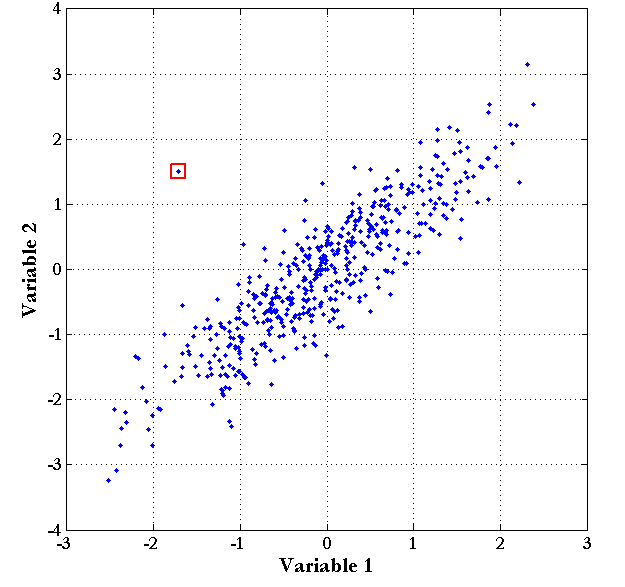
\includegraphics[width=0.5\textwidth]{mahalanobis.png}
\caption[Mahalanobis distance]{In this simple example of a 2-dimensional space, the point enclosed by the red square clearly does not obey the distribution exhibited by the rest of the data points. Although the outlier does not sit at the center of either scale, there are quite a few points with more extreme values of both Variable 1 and Variable 2, so using Euclidean distance it would be tricky to detect this anomaly. The Mahalanobis distance, instead, would easily find this outlier.}
\end{figure}

As an intuitive explanation of how this distance works, consider the problem of estimating the probability that a test point in $N$-dimensional space belongs to a set, where we are given sample points that definitely belong to that set.
The first step would be to find the average or center of mass of the sample points.
Intuitively, the closer the point in question is to this center of mass, the more likely it is to belong to the set.
However, we also need to know if the set is spread out over a large range or a small range, so that we can decide whether a given distance from the center is noteworthy or not.
The simplistic approach is to estimate the standard deviation of the distances of the sample points from the center of mass.
If the distance between the test point and the center of mass is less than one standard deviation, then we might conclude that it is highly probable that the test point belongs to the set.
The further away it is, the more likely that the test point should not be classified as belonging to the set.
This intuitive approach can be made quantitative by defining the normalized distance between the test point and the set to be the \emph{Z-Score} (as explained before) of that point.
The drawback of the above approach is that we assume that the sample points are distributed about the center of mass in a spherical manner.
When the distribution of the points is non-spherical, for example ellipsoidal, then we would expect the probability of the test point belonging to the set to depend not only on the distance from the center of mass, but also on the direction.
In those directions where the ellipsoid has a short axis the test point must be closer, while in those where the axis is long the test point can be further away from the center.
Putting this on a mathematical basis, the ellipsoid that best represents the set's probability distribution can be estimated by building the covariance matrix of the samples.
The Mahalanobis distance is simply the distance of the test point from the center of mass divided by the width of the ellipsoid in the direction of the test point.

From a mathematical point of view, if we consider two points $x$ and $y$, which belong to a multi dimensional space of $N$ dimension, the Mahalanobis distance between them is defined as:

\begin{center}
\Large
$d(x,y) = \sqrt{(x - y)S^{-1}(x - y)}$
\end{center}

Where $S^{-1}$ is the inverse of the covariance matrix ($N \times N$ for $N$ dimensions), calculated with the usual formula.

So, the distance computation between two points is slightly more complicate (because we need to calculate the inverse of the correlation matrix, and this step can cause some problems when the analyzed dimensions are linearly interdependent, making the covariance matrix singular), but we don't need any prior data normalization such as Z-Score.
Mahalanobis distance has already been used together with clustering algorithms \cite{mahal}, but not in the network anomaly detection field.


%esempio

\section{Clustering algorithm}

\subsection{\emph{K-Means++} Algorithm}
At this point, the data is ready to be directly processed by the clustering algorithm.
In this proposed approach, we used two types of pretty famous algorithms. The first is called \emph{K-Means++}. It is a fairly recent version of the classic \emph{K-Means} algorithm (which is already used to perform network anomaly detection, but using metrics from \emph{NetFow} \cite{kmeans}), extremely popular in literature and widely used for many applications.
The main reason why we chose this algorithm is that it provides slightly better results than its predecessor, and, after a careful process of research in the scientific literature, it seems that it has never been used before in the field of network anomaly detection with \emph{non-NetFlow} data. 

Before introducing how the algorithm works, it is probably worth to explain something about the original \emph{K-Means} implementation.
\emph{K-Means} aims to partition a data set, consisting of $n$ points in a multi-dimensional space, into $k$ clusters, in which each point belongs to the cluster with the nearest mean. It attempts to find the centers of natural clusters in the data with an iterative refinement approach.
From a more formal point, given a set of points $(x_1, x_2, etc., x_n)$, \emph{K-Means} will partition the $n$ points into $k$ clusters ($k < n$) $S = {S_1, S_2, etc., S_k}$ in order to minimize the sum of the squared error for each cluster:

\begin{center}
\Large
$\sum_{i=1}^{k}{\sum_{x_j \in S_i}{\left \| x_j - \mu_i  \right\|^2}}$
\end{center}

where $\mu_i$ is the centroid representing all the points assigned to the cluster $S_i$.

So, the general procedure follows a simple and easy way to classify a given data set through a certain number of clusters (fixed a priori).
The main idea is to define $k$ centroids, one for each cluster.
These centroids must be placed in a smart way because different locations causes different results.
So, one of the best choices is to place them as much as possible far away from each other.
The next step is to take each point belonging to a given data set and associate it to the nearest centroid.
When no point is pending, the first step is completed and an early grouping is done.
At this point, it is needed to re-calculate $k$ new centroids for the clusters resulting from the previous step.
After these $k$ new centroids are computed, a new binding has to be done between the same data set points and the nearest new centroid.
A loop has been generated. As a result of this loop the $k$ centroids will change their location step by step until no more changes are done, and centroids do not move any more.

The basic version of the algorithm can be then summarized in four simple steps:

\begin{enumerate}
\item Place $K$ points into the space represented by the objects that are being clustered. These points represent initial group centroids;
\item Assign each object to the group that has the closest centroid;
\item When all objects have been assigned, recalculate the positions of the $K$ centroids;
\item Repeat Steps 2 and 3 until the centroids no longer move. This produces a separation of the objects into groups from which the metric to be minimized can be calculated;
\end{enumerate}

The metric to be minimized can be any distance measure that can return a numeric value for the ``proximity'' between two points in the space.
As said before, in this approach we mainly used Euclidean distance (with a previous Z-Score normalization step) and Mahalanobis distance.

\begin{figure}
\centering
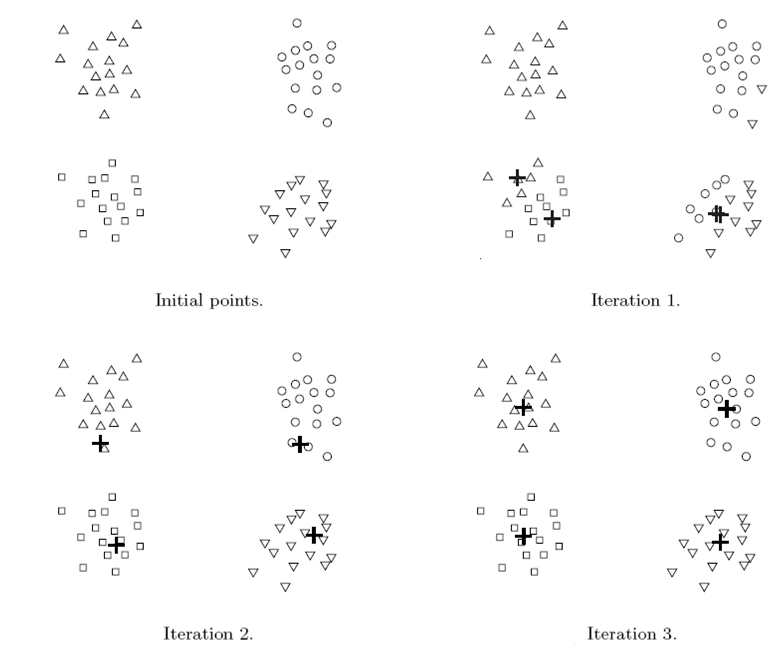
\includegraphics[width=0.8\textwidth]{kmeans1.png}
\caption[\emph{K-Means} iterations]{This figure shows some snapshots captured at each iteration of the \emph{K-Means} algorithm. The data is represented in a two-dimensional space, and the parameter k is set to 4. During the initialization step, centroids are randomly chosen.}
\end{figure}

It can be proved that the \emph{K-Means} procedure will always terminate, but it does not necessarily find the most optimal configuration, corresponding to the global objective function minimum.
This is mainly because the algorithm is significantly sensitive to the initial randomly-selected cluster centroids. This issue can be partially solved by running the procedure multiple times, to reduce this ``greedy'' effect.
The other possibility is to use a bit more complex initialization phase (instead of randomly choosing the first $K$ centroids), and this is exactly what happens in the \emph{K-Means++} variant, used in our model.

To conclude this first overview, it is quite simple to guess what are the main weaknesses of this approach:

\begin{itemize}
\item The way to initialize the centroids is extremely critical, and can severely affect the clustering results;
\item It frequently happens that suboptimal partitions are found;
\item The results heavily depend on the metric used to measure $ \left \| x - \mu  \right\| $, and this is why we tried to use measures which take into account the statistical dependence between each dimension;
\item The results depend on the value of $k$, and the algorithm is not able to determine it automatically, and so it must be chosen a priori. The correct choice of $k$ is often ambiguous, with interpretations depending on the shape and scale of the distribution of the points in the data set. In addition, it is interesting to notice that increasing $k$ will always reduce the amount of error in the resulting clustering, to the extreme case of no error if each data point is considered its own cluster (when $k$ equals the number of data points). Then, the optimal choice of $k$ must be a balance between maximum compression of the data using a single cluster, and maximum accuracy by assigning each data point to its own cluster;
\item There are some limitations when the clusters have a non-spherical, non-elliptical or different densities. This is a typical problem of \emph{K-Means} and all its variants. 
However, during our tests, we noticed that the algorithm behaves quite well in separating network data into different clusters in order to detect outliers, and this is probably due to the particular type of metrics used, or to the simple fact that we are more interested in detecting what is ``far'' from the clusters, rather than the clusters themselves;
\end{itemize}

\begin{figure}
\centering
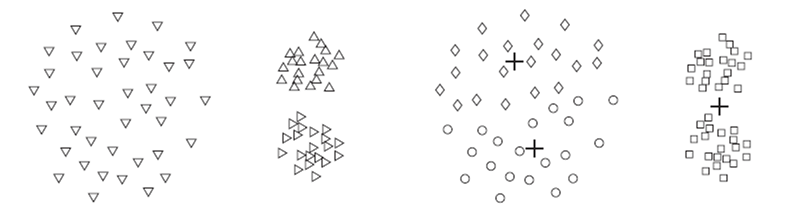
\includegraphics[width=\textwidth]{kmeans2.png}
\caption[\emph{K-Means} iterations]{This figure shows how \emph{K-Means} fails to detect the three clusters, because the two smaller ones are much more denser than the larger one.}
\end{figure}

Obviously the use of the \emph{K-Means} algorithm not only entails disadvantages, because with its simple logic it is probably the fastest among clustering algorithms, and from a computational point of view the needed resources are very limited.
In particular, the memory needed is $O((m + K)n)$, where $m$ is the number of points and $n$ is the number of dimensions (basically the only data structures needed are the original matrix containing the samples and the matrix containing centroids' coordinates in the multi-dimensional space).
The time requirement is $O(I \ast K \ast m \ast n)$, where $I$ is the number of iterations required for convergence, and this value is usually very small, since most of the changes typically occur during the first few iterations.
Therefore, the algorithm is basically linear in $m$, the number of points, and so it is relatively efficient, compared to other approaches.

Now that the basic version of the \emph{K-Means} algorithm has been explained, it is possible to describe one of his successors, the \emph{K-Means++}, which was used in this model.
As it has already been said, choosing the proper initial centroids is the key step of this algorithm, and a common, but poor, approach is to choose them randomly.
This choice has a lot of drawbacks: using a random initialization, the \emph{K-Means} will find a local optimum solution, but it can miss the ``big picture'' of the entire multi-dimensional space. 
For example, if the data set has well separated clusters, and the initial centroids are chosen uniformly at random, it is relatively easy to get two centers in one clusters, as shown in figure:

\begin{figure}
%\centering
\subfloat[Initial centroids are completely randomly chosen]
{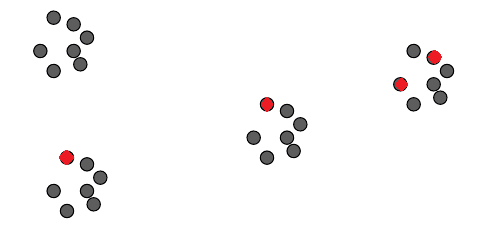
\includegraphics[width=0.5\linewidth]{kmeanspp1.png}}
\subfloat[Detected clusters do not represent a globally optimal solution]
{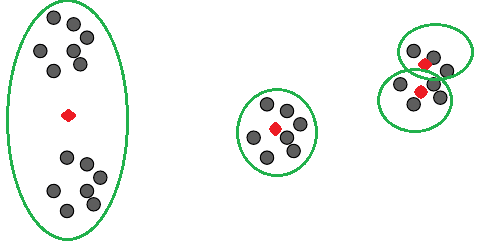
\includegraphics[width=0.5\linewidth]{kmeanspp2.png}}
\end{figure}

The \emph{K-Means++} algorithm addresses this problem by intelligently choosing the initial coordinates of centroids, before proceeding with the standard \emph{K-Means} iterations.
The initialization procedure is pretty simple, and it consists in selecting the initial centers iteratively: more specifically, if we define as $D(x)$ the distance from the point $x$ to nearest existing center, $x$ will be chosen as a new initial center with a probability proportional to $D(x)^2$.
The full steps for the algorithm are then:

\begin{enumerate}
\item Choose one center uniformly at random from among the data points;
\item For each data point $x$, compute $D(x)$, the distance between $x$ and the nearest center that has already been chosen;
\item Add one new data point at random as a new center, using a weighted probability distribution where a point $x$ is chosen with probability proportional to $D(x)^2$;
\item Repeat Steps 2 and 3 until $k$ centers have been chosen;
\item Proceed using standard \emph{K-Means} clustering;
\end{enumerate}

This method gives out considerable improvements in the final error of the clustering, and although the initial selection in the algorithm takes extra time, the \emph{K-Means} part itself converges very fast after this initialization and thus the algorithm actually lowers the computation time too.
The \emph{K-Means++}'s authors have also mathematically proven \cite{kmeanspp} that the algorithm is guaranteed to find a solution that is $O(log (k))$ competitive to the optimal \emph{K-Means} solution.

\subsection{\emph{DBSCAN} Algorithm}

The other algorithm used in the approach is \emph{DBSCAN}.
This method is very different from the previous \emph{K-Means}, and in our case, as it can be seen from the results in the next section, it performed much more better, with the disadvantage of increasing complexity.

\emph{DBSCAN} is the typical density-based clustering algorithm, so basically it locates regions of high density that are separated from one another by regions of low density inside the multi-dimensional space.
The algorithm itself is pretty simple (although much more complicated than \emph{K-Means}), and it is completely based around the concept of ``density'' for each point.
This density for a specific point is estimated by counting the number of points within a specified radius, \emph{Eps}, of that point.
One thing to notice is that we are talking about ``radius'', but from a mathematical point of view this is only correct if we use the Euclidean distance to determine whether two points are close together (less than \emph{Eps}), because, if we use a different distance measure such as the Mahalanobis one, the concept of neighborhood for a point is not ``spherical'' anymore, but depends on the statistical relationships between the different dimensions, and from our results the algorithm works quite well even with complex distance measurements.

To illustrate how the algorithm works, it is necessary to introduce the concept of ``label'' for a point, according to the density definition.
Each point can be labeled as:

\begin{itemize}
\item \textbf{Core}: This point is in the interior of a density-based cluster. It is a core point if the number of points within a given neighborhood around the point as determined by the distance measure and the user-specified distance parameter, \emph{Eps}, exceeds a certain threshold, \emph{MinPts}, which is also a user-specified parameter;
\item \textbf{Border}: A border point is not a core point, but falls within the neighborhood of a core point. A border point can fall within the neighborhoods of several core points;
\item \textbf{Noise}: A noise point is any point that is neither a core point nor a border point. Usually it is not worth to identify these points. Instead, in our model, this is probably more important than determining the clusters themselves, since every noise point represents an outlier in the data set;
\end{itemize}

\begin{figure}
\centering
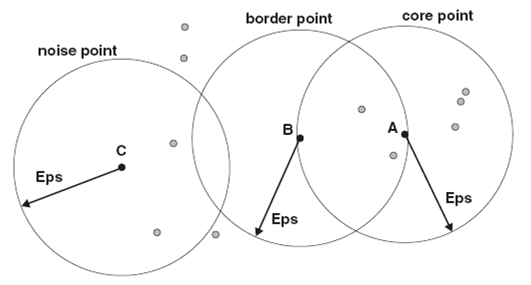
\includegraphics[width=0.8\linewidth]{dbscan.png}
\caption[\emph{DBSCAN} points]{Labels assigned by \emph{DBSCAN} algorithm to the points of a two-dimensional space.}
\end{figure}

The algorithm requires then two parameters: \emph{Eps} and the minimum number of points required to form a cluster, \emph{MinPts}.

Given this definitions, the \emph{DBSCAN} algorithm works by putting in the same cluster any two core points that are close enough (within a distance \emph{Eps} of one another). Likewise, any border point that is close enough to a core point is put in the same cluster as the core point. Noise points are not absorbed in any cluster.
The algorithm (modified to fit the needs of our application) can then be summarized in the following steps:

\begin{enumerate}
\item Label all points as core, border or noise points;
\item Trigger an alarm for each detected noise point (this step is peculiar for the anomaly detection application, otherwise noise points can simply be eliminated);
\item  Put an edge between all core points that are withing \emph{Eps} of each other;
\item Make each group of connected core points into a separate cluster;
\item Assign each border point to one of the clusters of its associated core points;
\end{enumerate}

It is quite evident that the biggest advantage of using this algorithm is that it is not required to know the number of clusters in the data a priori, because the optimal number is automatically detected (as opposed to \emph{K-Means}). On the contrary, the main drawbacks are:

\begin{itemize}
\item The results of the clustering heavily depend on the distance measure, and, especially for high-dimensional data, the distance metric can become almost useless (but we already tried to solve this issue using \emph{PCA});
\item It does not respond well to data sets with varying densities. Fortunately, during our tests we saw that basically the network metrics we analyzed do not suffer from this problem;
\end{itemize}

From a computational point of view, the time complexity of the algorithm is $O(m \times t)$, where $m$ is the number of points and $t$ is the time to find points in the neighborhood of a certain point. In the worst case, this complexity is then $O(m^2)$, even if, in low-dimensional spaces, there are several data structures that help keep low this component. The space requirement, even for high-dimensional data, is $O(m)$ because it is only necessary to keep a small amount of data for each point (e.g. the label of each point).

\section{Validating the clustering model}

\subsection{Data set and anomalies}
In order to test the accuracy and the precision of the proposed clustering method, we need to verify the behavior using real traffic.
This is a very tricky part of the job, since the given traffic set may not include all of the anomalies (mainly security related anomalies during this specific tests) we may want to test the detection method against. Moreover, with unlabeled data, it is not even clear if these anomalies exist and what false positive and false negative rates of detecting them are (because we don't know exactly how many they are).
For solving this issue, we do the analysis using synthetic anomalies generation. By generating synthetic anomalies, we have complete control over the behavior of the injected data and the magnitude of the anomalies. Furthermore, any number of anomalies can be generated simultaneously to better understand how the system works in the multi-dimensional space.
To perform synthetic anomalies, we first generate a lot of small traffic traces containing some threats that we would want to detect, and then we inject this data (at time intervals randomly chosen) in a real and extremely long network traffic trace.
The capture we use collects all the traffic (bidirectional) which passed between the main router of a medium-sized IT company and the uplink to the ISP.
To achieve the injection, several UNIX tools are used (nmap\footnote{\url{http://www.nmap.org}}, nessus\footnote{\url{www.nessus.org}}, wireshark\footnote{\url{http://www.wireshark.org/}}, mergecap\footnote{\url{http://www.wireshark.org/docs/man-pages/mergecap.html}}, etc.), and the result is a huge data set where we know exactly where the anomalies are, so that we can estimate the precision of the anomaly detector.
We only consider inbound anomalies (basically security threats generated from external entities): the source addresses involved in the incidents are outside the considered network and the destination addresses are inside it. We expect that the results for outbound anomalies are qualitatively similar.
Since the whole data set is extremely large (more than four months), we use as aggregation interval one hour, so that for every hour the acquisition process computes a points which fits in the multi dimensional space that will be given as input to the clustering algorithm (the details about the implementation and how we process the data will be given later).

We use two types of data sets, in order to try to resolve some of the problems inherent in the \emph{K-Means} algorithm:

\begin{itemize}
\item \textbf{Entire}: in this case the data set is seen as one entire block, without making any manual separation of the samples. The clustering algorithm will then run once on all the samples for the entire time period considered;
\item \textbf{Divided}: In this case, we consider the seasonality of the data set (mainly an hourly seasonality), and so, we divide the data set in 24 subsets, each one containing the samples related to that specific time of the day. By temporally dividing the data set, it is expected that the network pattern for each subset will be more constant, and this thing helps a lot a clustering algorithm like \emph{K-Means++}, where it is necessary to specify in advance the number of clusters to be obtained. Even if an improvement like this would help the \emph{DBSCAN} algorithm as well, we decided to introduce this feature only where strictly necessary in order to improve the results of the tests, because it is a rough approximation of the real data. Then, we decided to skip this type of data set when using \emph{DBSCAN}, since this algorithm is able to automatically discover the best number of clusters and it performed quite well compared to the other options. By using this approach, we execute one independent instance of the algorithm for every subset;
\end{itemize}

\subsection{Tuning \emph{K-Means++} parameters}

The only parameter for this algorithm is \emph{k}, or the number of clusters that we want as output.
The correct choice of this value is absolutely ambiguous, with interpretations depending on the shape and scale of the distribution of points in a data set and the desired clustering resolution of the user. In addition, increasing \emph{k} without penalty will always reduce the amount of error in the resulting clustering, to the extreme case of no error if each data point is considered its own cluster \footnote{Of course this is just an extreme case, since from a practical point of view it would be totally useless and meaningless}. So, the optimal choice of \emph{k} will strike a balance between maximum compression of the data using a single cluster, and maximum accuracy by assigning each data point to its own cluster (the good compromise between these two extreme situations is the correct number of clusters needed to model the typical pattern of the metrics, highlighting the outliers). Basically, after performing many tests, we can say that this parameter heavily depends on what kind of data set we use. In particular:

\begin{itemize}
\item if the data set considered is \textbf{entire}, the parameter depends on how we detect outliers. In our case, we identify the outliers as the points which belongs to the smallest clusters, and even those which are too far (over a certain threshold) from their centroids, with respect to the average of the points in the same cluster. 
\item if the data set considered is \textbf{divided}, a quite good compromise is achieved by setting the parameter to 2, especially when the dimensions considered in the analysis can capture quite well the variation caused by abnormalities (the outliers will be identified as the points belonging to the smallest of the two clusters, if exists);
\end{itemize}

\subsection{Tuning \emph{DBSCAN} parameters}

The greatest advantage of density-based clustering algorithms like \emph{DBSCAN} is that the number of clusters is automatically determined during the processing, and it depends only on the data set. 
Unfortunately, there are other parameters which severely affect the results of the algorithm, and the most difficult one to estimate is the \emph{Eps} value.
The \emph{Eps} value is a constraint to the results. If the \emph{Eps} value is set to a too low value, some points are classified as noise points instead of being aggregated to a cluster.
Using larger values for \emph{Eps} partially solves this problem, but doing so the algorithm will not detect some anomalies.
To estimate the \emph{Eps} value, we use a simple but effective heuristic which was originally proposed by the \emph{DBSCAN} authors \cite{dbscan}. 
This heuristic is based on the following observation. Let \emph{d} be the distance of a point \emph{p} to its \emph{k}-th nearest neighbor, then the \emph{d}-neighborhood of \emph{p} contains exactly \emph{k+1} points for almost all points \emph{p}.
The \emph{d}-neighborhood of \emph{p} contains more than \emph{k+1} points only if several points have exactly the same distance \emph{d} from \emph{p}, which is quite unlikely.
For a given \emph{k} we define a function \emph{k}-dist, mapping each point of the data set to the distance from its \emph{k}-th nearest neighbor. When sorting the points of the data set in descending order of their \emph{k}-dist values, the graph of this function gives some hints concerning the density distribution in the database. This graph is called the sorted \emph{k}-dist graph. If we choose an arbitrary point \emph{p}, set the parameter \emph{Eps} to \emph{k}-dist(\emph{p}) and set the parameter \emph{MinPts} to \emph{k}, all points with an equal or smaller \emph{k}-dist value will be core points. We estimate the threshold point as the first point in the first knee of the sorted \emph{k}-dist graph. All points with a higher \emph{k}-dist value are considered to be noise, and all other points are assigned to some cluster.
To detect the knee of this curve, we developed a really simple (and unfortunately not perfect) algorithm which uses some measures like moving average and the derivative of the signal in order to estimate this value. In general, this seems to work quite good when the anomalies are particularly obvious (such as the ones affecting the bandwidth), while it has some problems in detecting more ``thiner'' outliers.
For the other paramer, \emph{MinPts}, we tried several values, and there is no optimal value for this parameter, since it heavily depends on the type of traffic that is being analyzed.
For our tests, several attempts were made at intervals from 3 to 50 points per cluster.
An example of this kind of calibration is shown in figure \ref{img:kdist}.

\begin{figure}[h]
%\centering
\subfloat[k-dist graph for the first test scenario (distributed bandwidth flood). With k=30, the algorithm estimates Eps=2.1]{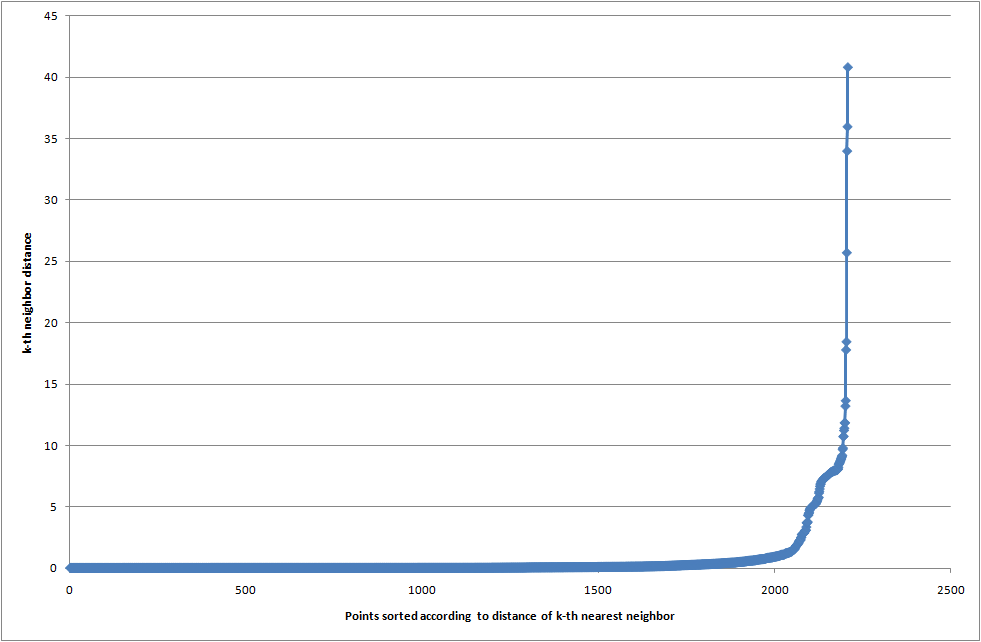
\includegraphics[width=0.5\linewidth, height=5cm]{kdist1.png}}
\subfloat[k-dist graph for the second test scenario (syntetic vertical scan). With k=30, the algorithm estimates Eps=17.3]{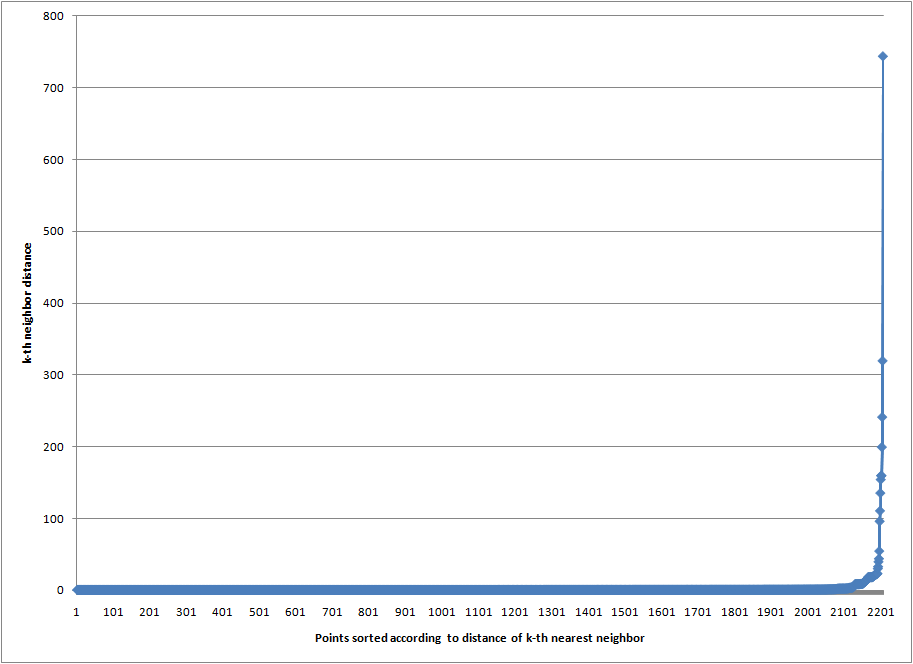
\includegraphics[width=0.5\linewidth, height=5cm]{kdist2.png}}
\caption{k-dist-based DBSCAN calibration}
\label{img:kdist}
\end{figure}

\subsection{First example: synthetic distributed bandwidth flood}
Distributed bandwidth floods are one of the earliest and still active attacks in the Internet due to their ability to exploit the low bandwidth of endpoints in the Internet with a network of compromised low bandwidth hosts. While mechanisms are still being proposed and developed to prevent or reduce the effects of the attacks, they are still active in the Internet today. Although they are arguably one of the easiest attacks to detect (because they basically affect the network bandwidth), sometime it is more difficult to detect them, especially in large (and usually busy) networks.
For this test, we use a very simple distributed denial of service attack called ping flood.
In this situation, the attacker overwhelms the victim with \emph{ICMP} Echo Request (ping) packets. It only succeeds if the attacker has more bandwidth than the victim. The attacker hopes that the victim will respond with \emph{ICMP} Echo Reply packets, thus consuming outgoing bandwidth as well as incoming bandwidth.
Using this basic concept, we can extend the attack to a distributed environment. If you have a botnet of some thousands of zombies (which are the infected hosts that are available to automatically start the attack for us), each one can generate an attack similar to the previous one, and so the overall effect is amplified. In fact, we can add another level of complexity to this simple attack, by making source address spoofing (at \emph{IP} level) of the \emph{ICMP} packets generated by the zombies.
For validating the model, we create an anomaly detector with the following dimensions:

\begin{itemize}
\item \textbf{\emph{ICMP} packets}: number of \emph{ICMP} packets that have actually been transmitted on the wire;
\item \textbf{\emph{TCP} packets}: number of \emph{TCP} packets that have actually been transmitted on the wire;
\item \textbf{\emph{UDP} packets}: number of \emph{UDP} packets that have actually been transmitted on the wire;
\item \textbf{Unique \emph{IP} source addresses}: counts the number of distinct source \emph{IP} addresses;
\item \textbf{Unique \emph{IP} destination addresses}: counts the number of distinct destination \emph{IP} addresses;
\end{itemize}

For this test case, we create 100 anomalies, different in terms of hosts involved in the attack and bandwidth consumed, and then we manually inject them in the trace at random time intervals.

\begin{figure}
\centering
\subfloat[Unique \emph{IP} source addresses]{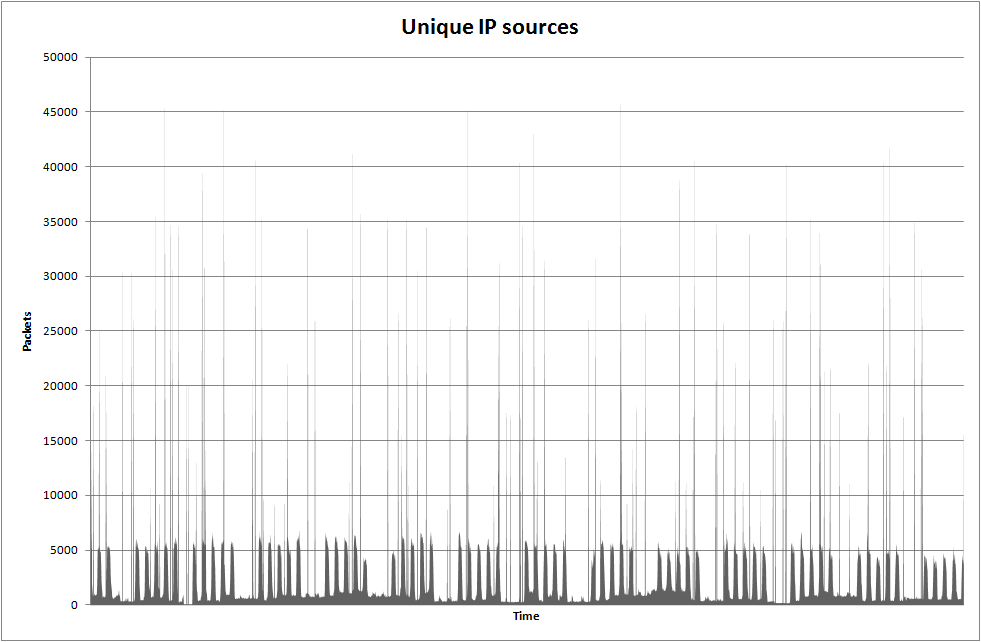
\includegraphics[width=0.5\textwidth]{ip_src.png}}
\subfloat[Unique \emph{IP} destination addresses]{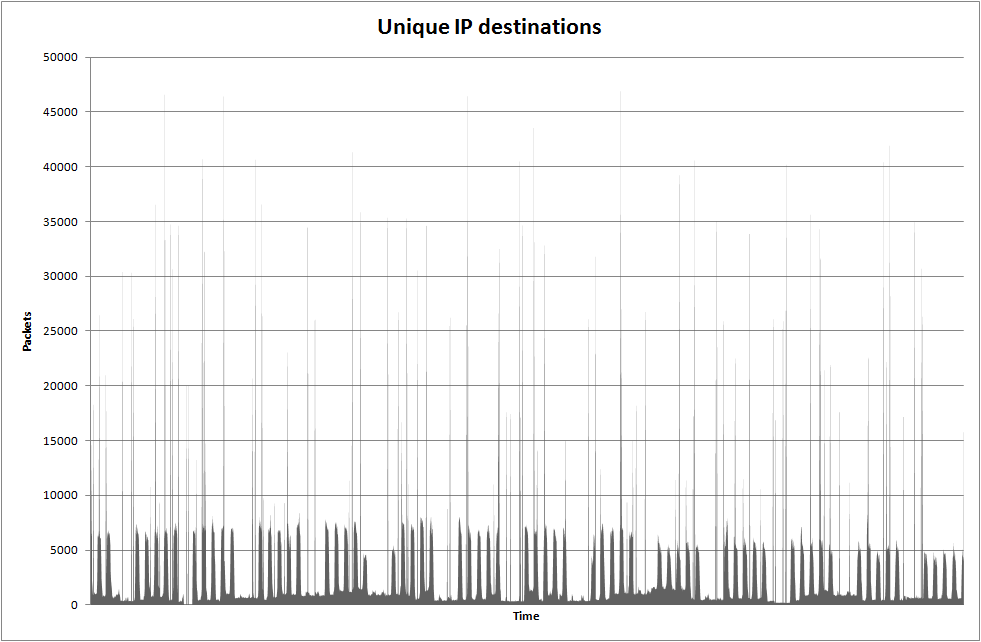
\includegraphics[width=0.5\textwidth]{ip_dst.png}}
\\
\subfloat[\emph{ICMP} packets]{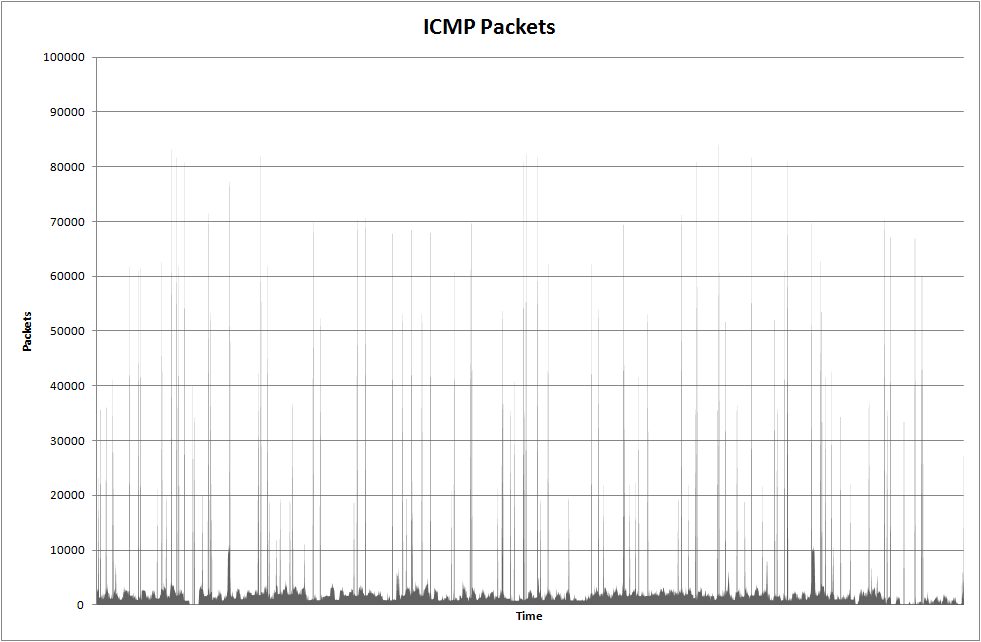
\includegraphics[width=0.5\textwidth]{icmp.png}}
\subfloat[\emph{UDP} packets]{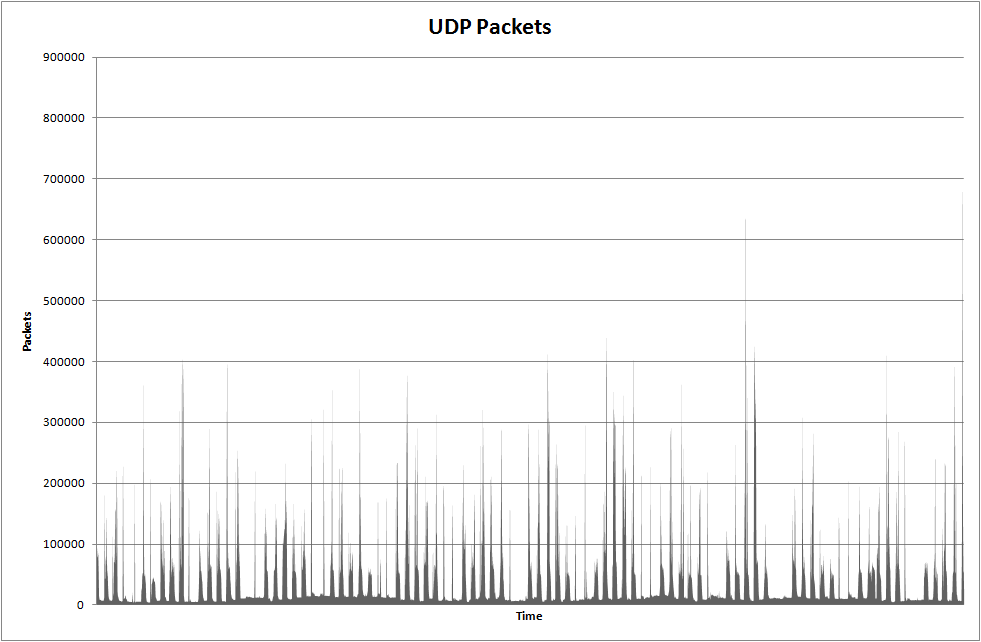
\includegraphics[width=0.5\textwidth]{udp.png}}
\\
\subfloat[\emph{TCP} packets]{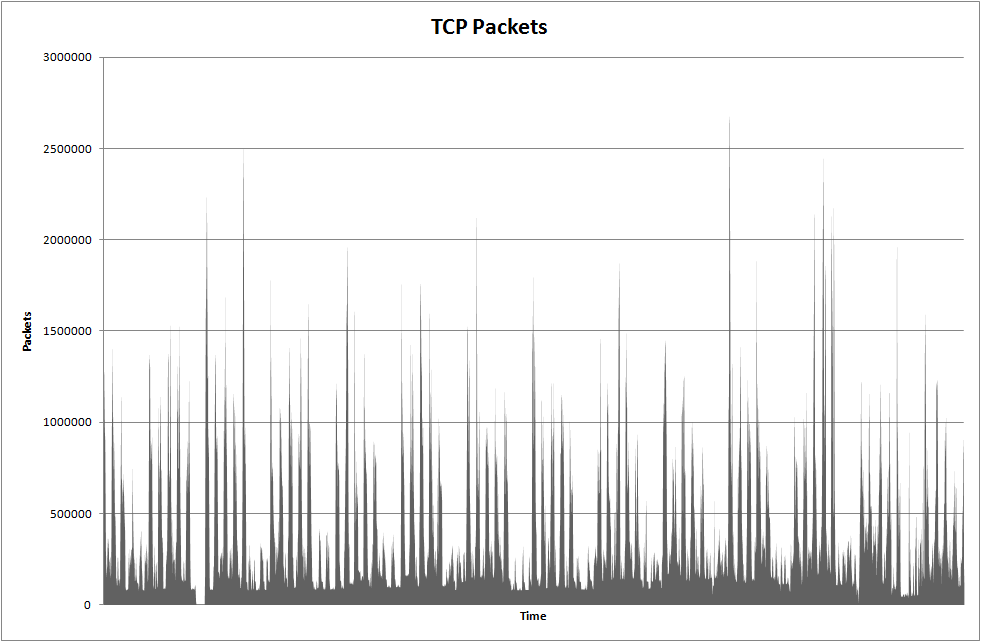
\includegraphics[width=0.5\textwidth]{tcp.png}}
\caption[Bandwidth flood - entire data set]{Bandwidth flood - entire version of the data set}
\end{figure}

\begin{figure}
\centering
\subfloat[\emph{ICMP} (hour 6)]{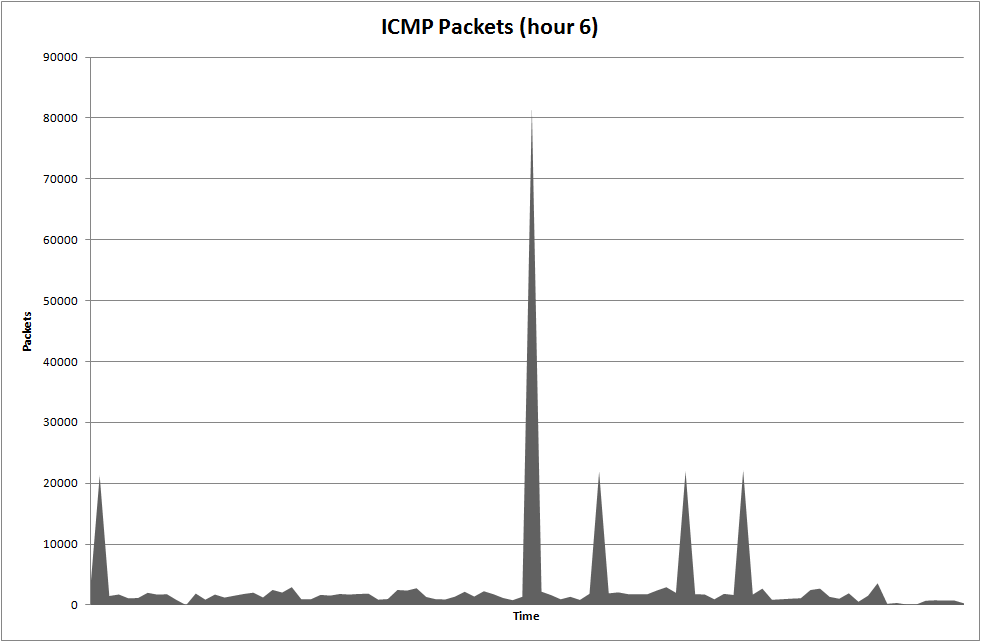
\includegraphics[width=0.33\textwidth]{icmp6.png}}
\subfloat[\emph{ICMP} (hour 12)]{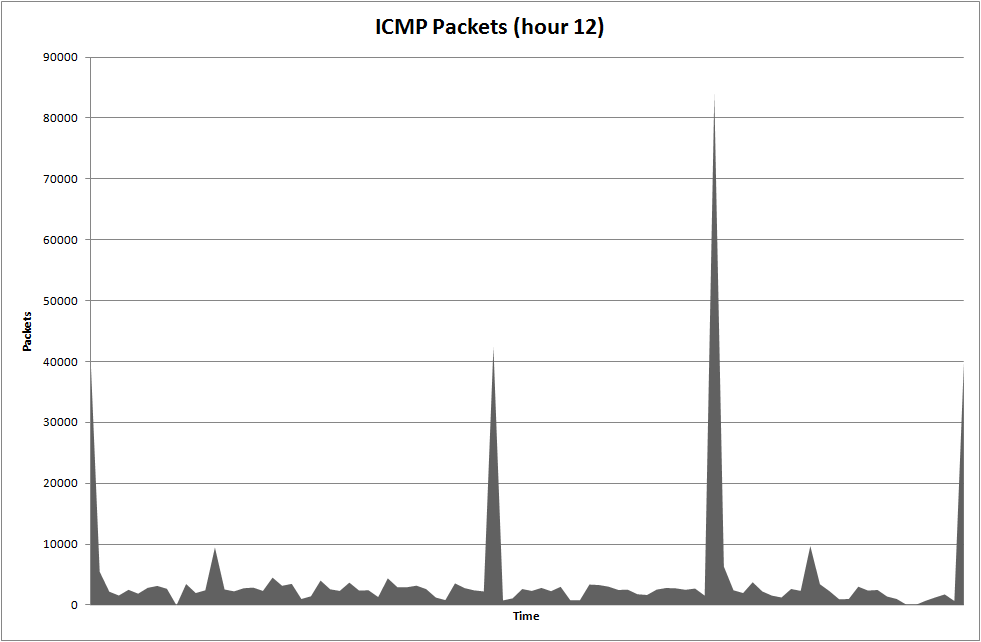
\includegraphics[width=0.33\textwidth]{icmp12.png}}
\subfloat[\emph{ICMP} (hour 18)]{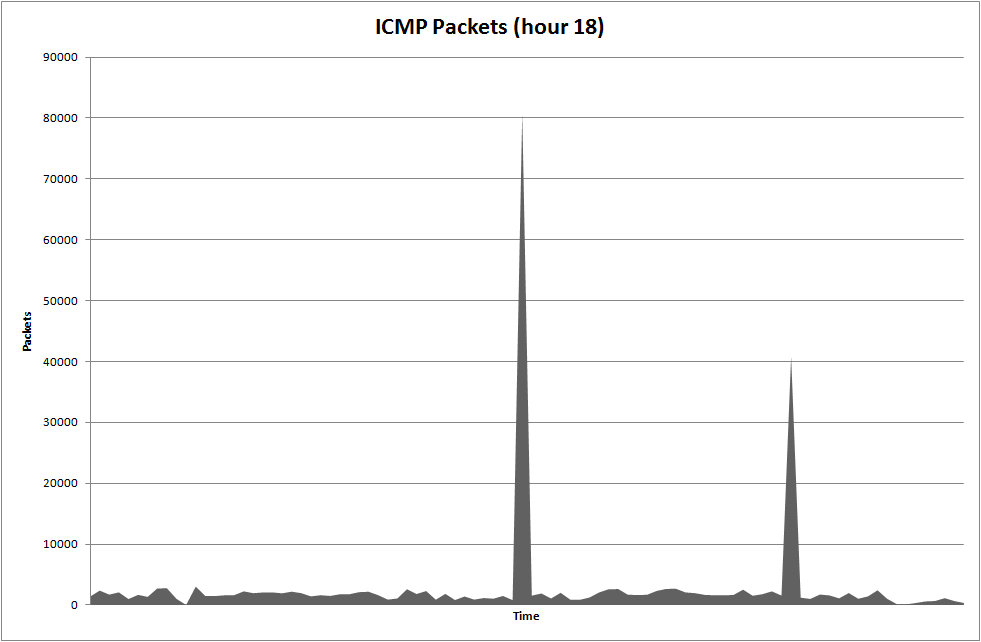
\includegraphics[width=0.33\textwidth]{icmp18.png}}
\\
\subfloat[\emph{UDP} (hour 6)]{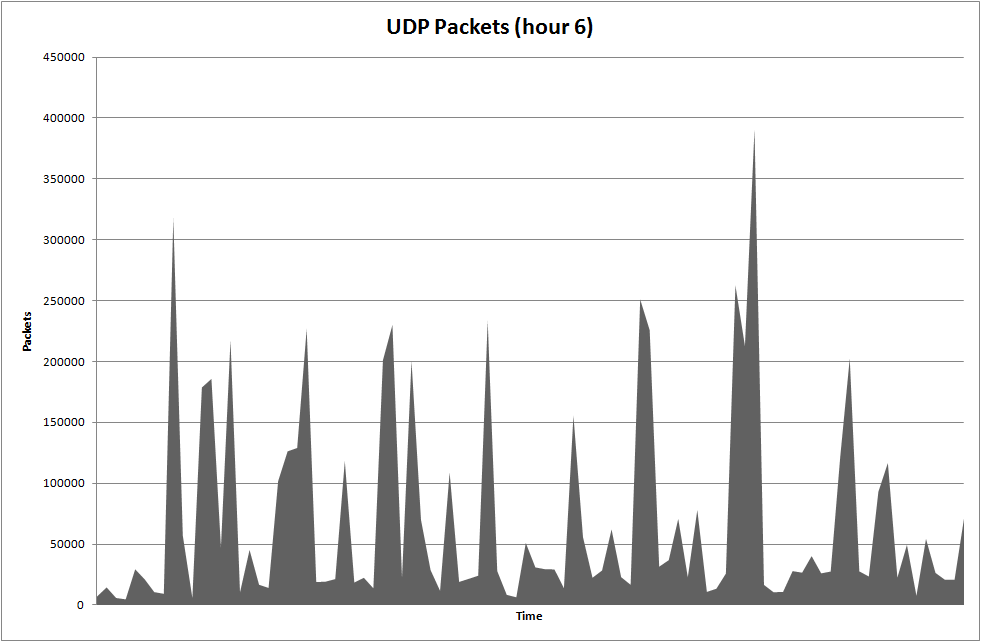
\includegraphics[width=0.33\textwidth]{udp6.png}}
\subfloat[\emph{UDP} (hour 12)]{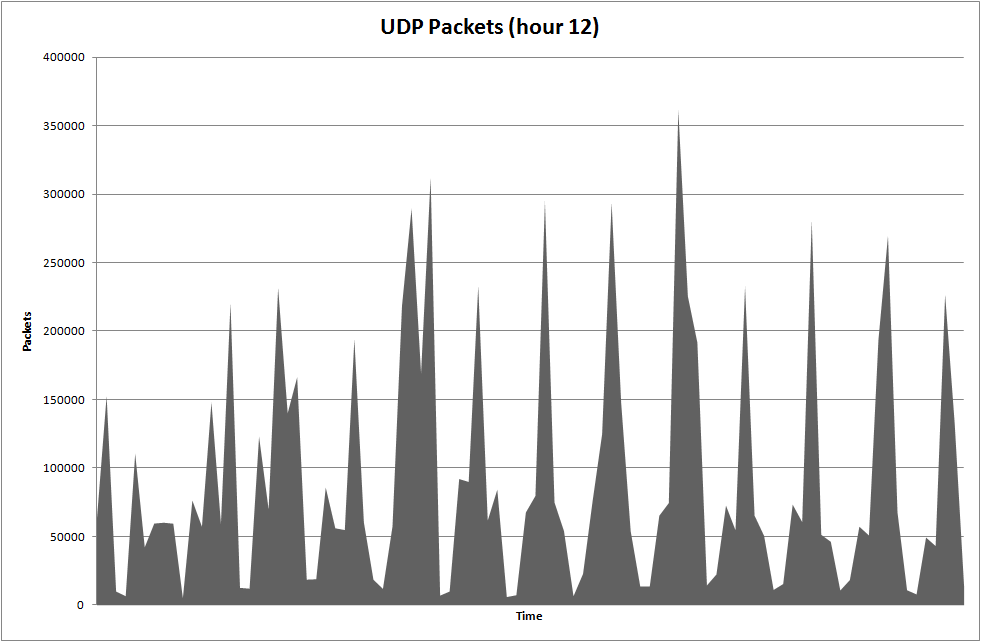
\includegraphics[width=0.33\textwidth]{udp12.png}}
\subfloat[\emph{UDP} (hour 18)]{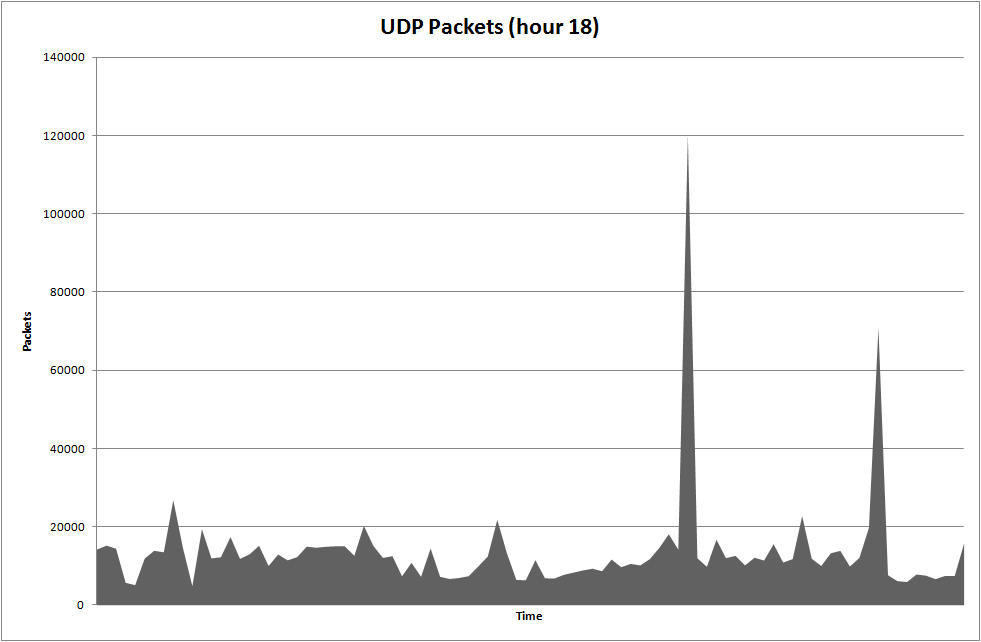
\includegraphics[width=0.33\textwidth]{udp18.png}}
\\
\subfloat[\emph{TCP} (hour 6)]{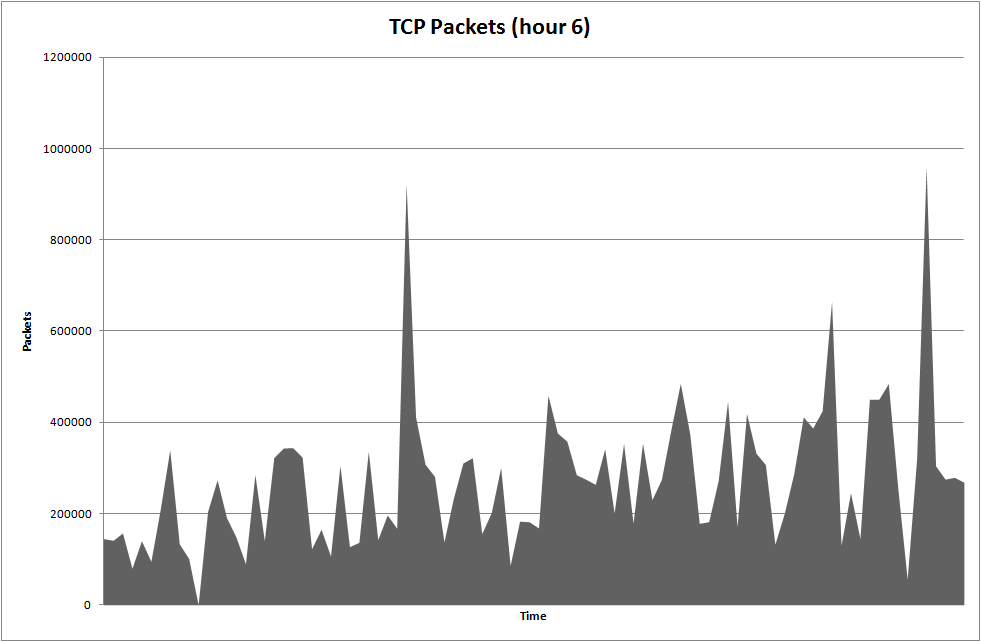
\includegraphics[width=0.33\textwidth]{tcp6.png}}
\subfloat[\emph{TCP} (hour 12)]{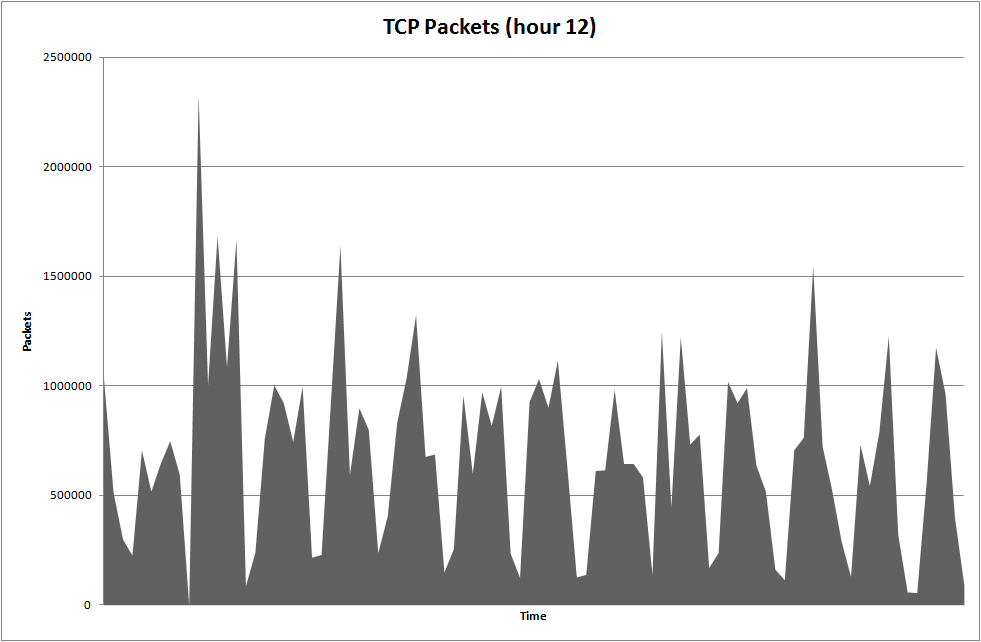
\includegraphics[width=0.33\textwidth]{tcp12.png}}
\subfloat[\emph{TCP} (hour 18)]{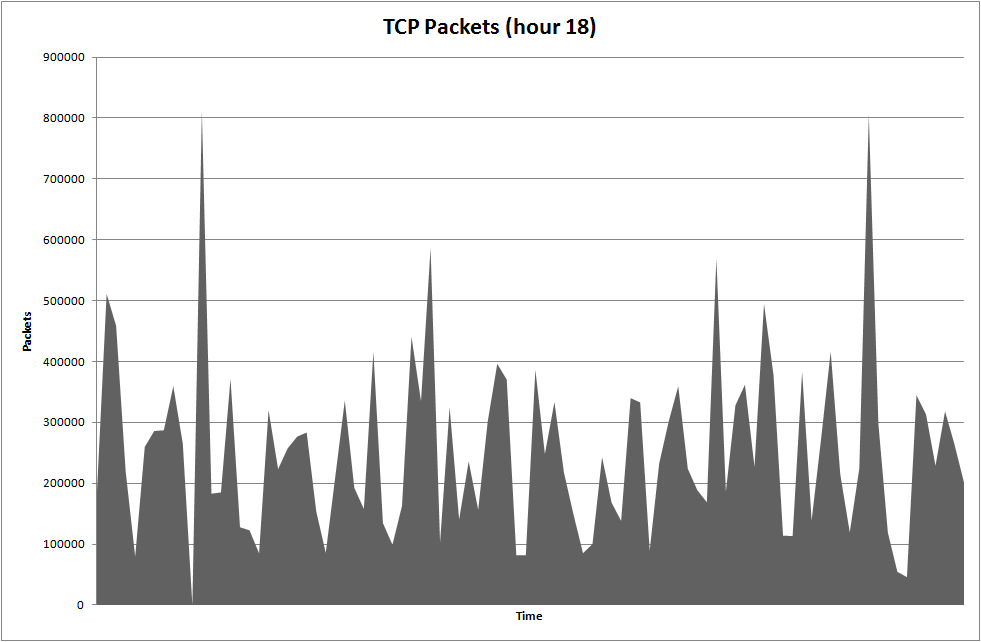
\includegraphics[width=0.33\textwidth]{tcp18.png}}
\\
\subfloat[\emph{IP} Sources (hour 6)]{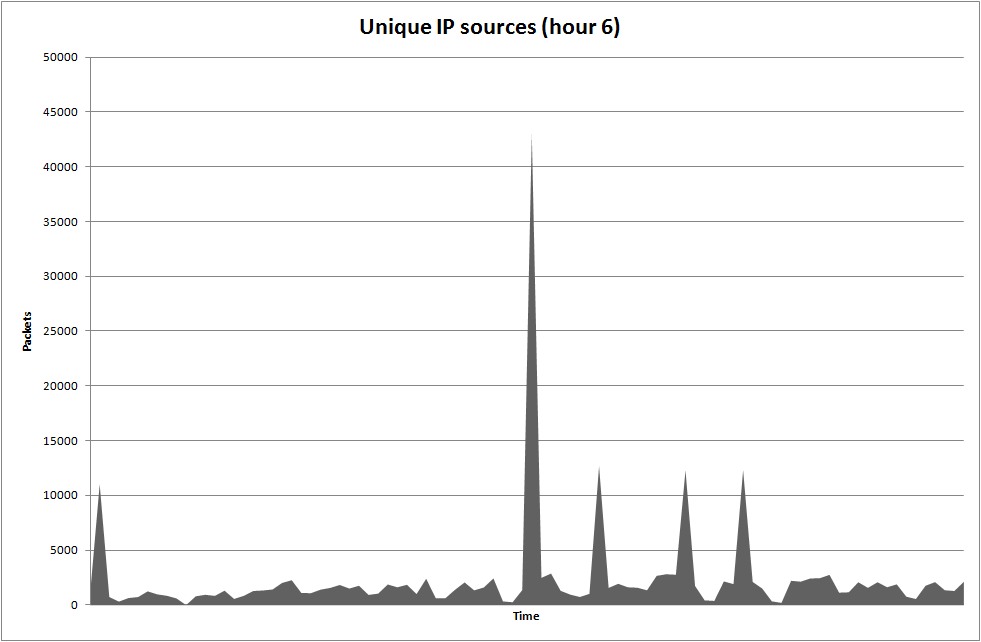
\includegraphics[width=0.33\textwidth]{ip_src6.png}}
\subfloat[\emph{IP} Sources (hour 12)]{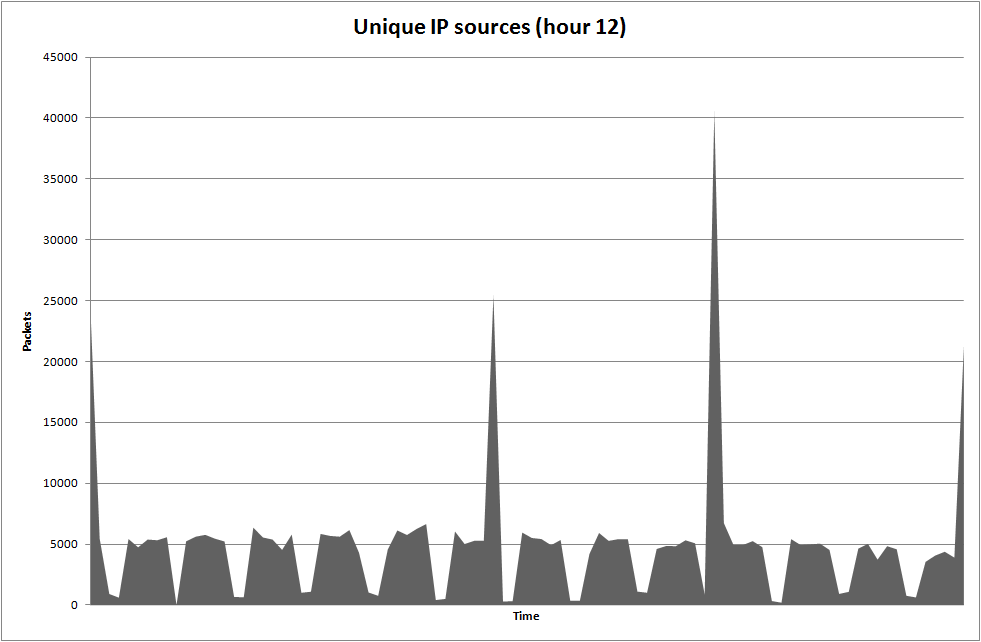
\includegraphics[width=0.33\textwidth]{ip_src12.png}}
\subfloat[\emph{IP} Sources (hour 18)]{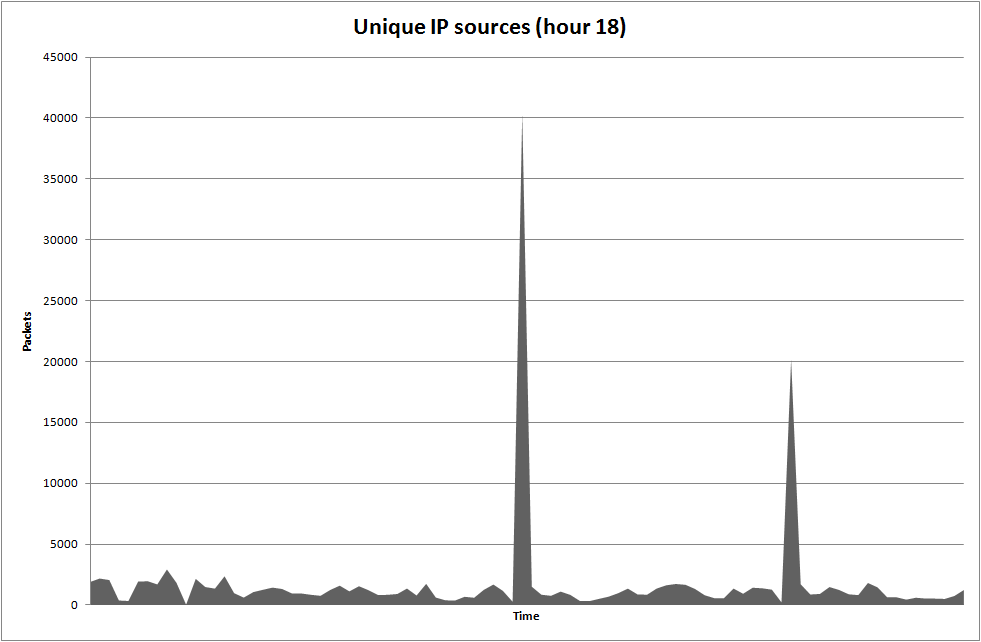
\includegraphics[width=0.33\textwidth]{ip_src18.png}}
\\
\subfloat[\emph{IP} Destinations (hour 6)]{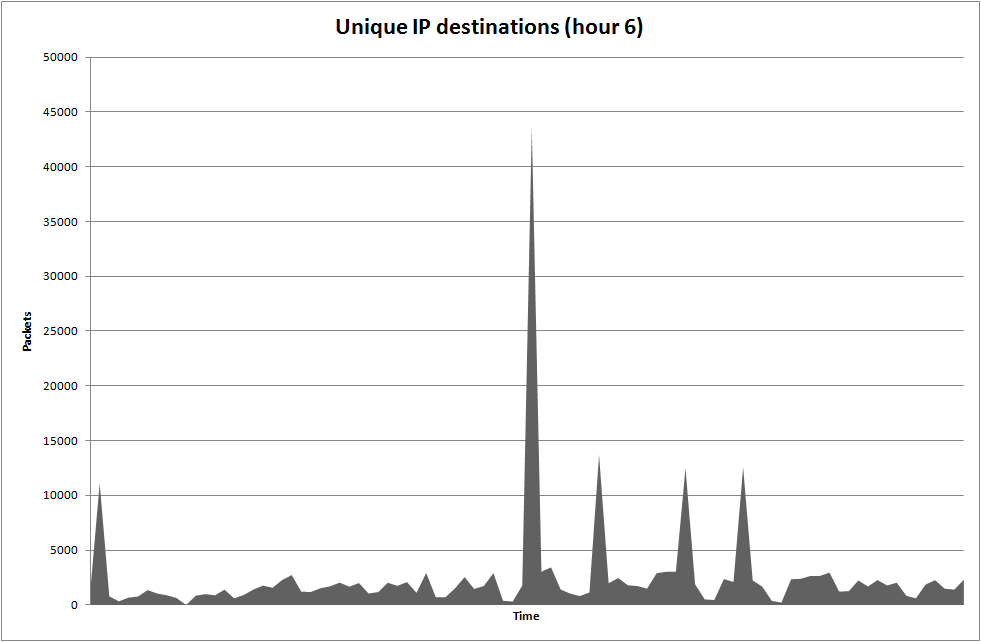
\includegraphics[width=0.33\textwidth]{ip_dst6.png}}
\subfloat[\emph{IP} Destinations (hour 12)]{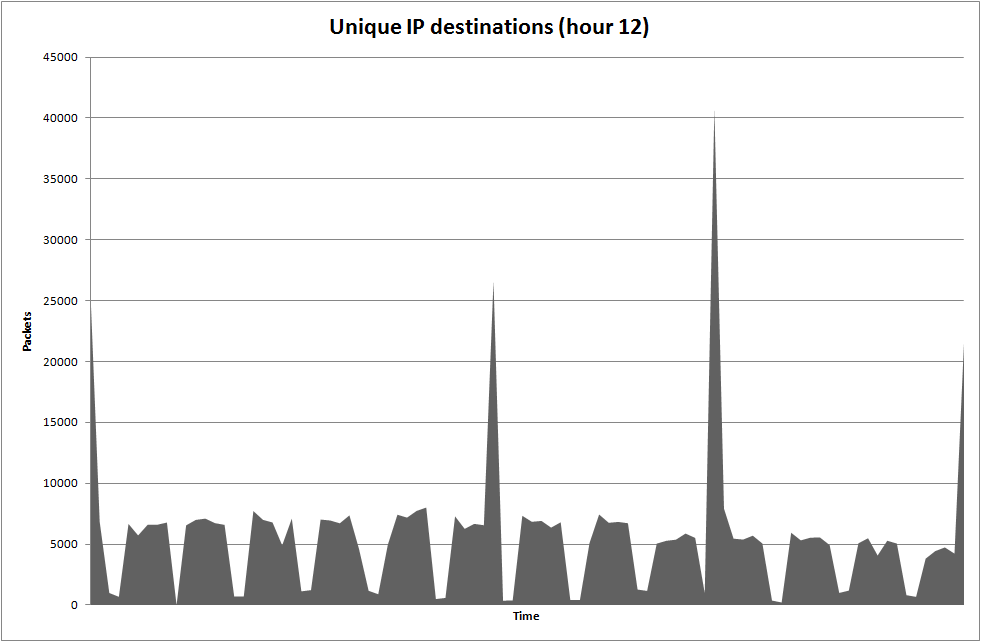
\includegraphics[width=0.33\textwidth]{ip_dst12.png}}
\subfloat[\emph{IP} Destinations (hour 18)]{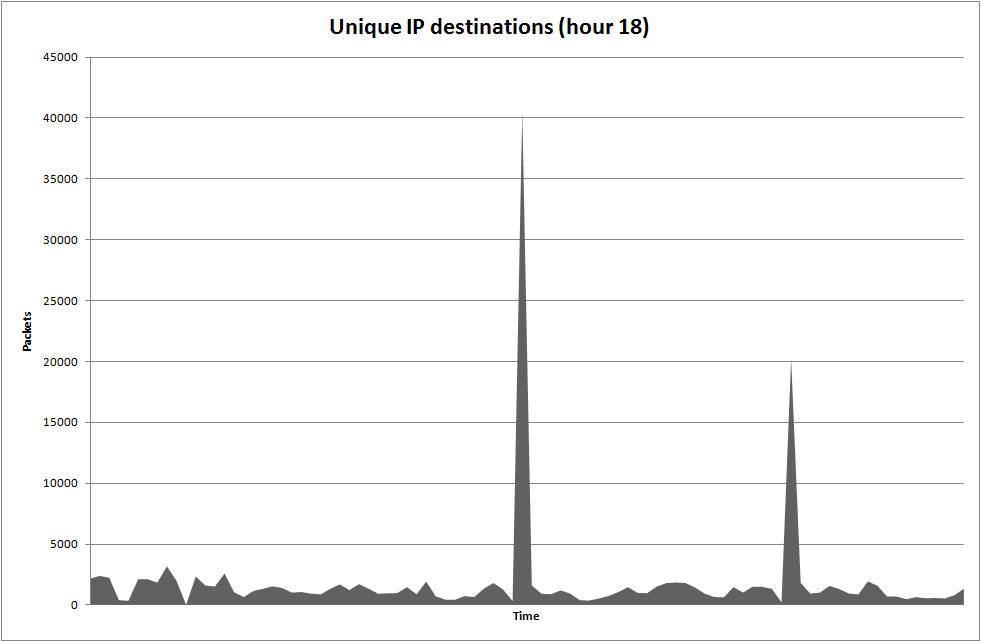
\includegraphics[width=0.33\textwidth]{ip_dst18.png}}
\caption[Bandwidth flood - divided data set]{Bandwidth flood - examples of the divided data set (only some hours are shown)}
\end{figure}

Then, we run the anomaly detector against the modified data. The results are shown in table \ref{tab-flood}. We mix several types of algorithm, preprocessing steps and distance measurements.
Please note that for the \emph{DBSCAN} algorithm we only use the entire data set (without dividing it), because it is not considered necessary.

\begin{center}
\begin{table}
\begin{tabular}{l|l|l|l|p{1.5cm}|p{1.5cm}|p{1.5cm}}
\hline
\hline
\multicolumn{7}{c}{Clustering results} \\
\hline
Algorithm & data set & Preprocessing & Distance & True positives & False positives & False Negatives \\
\hline
\emph{K-Means++} & Entire & Z-Score & Euclidean & 40 & 7 & 60 \\
\emph{K-Means++} & Entire & - & Mahalanobis & 46 & 108 & 54 \\
\emph{K-Means++} & Divided & Z-Score & Euclidean & 76 & 115 & 24 \\
\emph{K-Means++} & Divided & - & Mahalanobis & 84 & 170 & 16 \\
\emph{DBSCAN} & Entire & Z-Score & Euclidean & 73 & 8 & 27 \\
\emph{DBSCAN} & Entire & - & Mahalanobis & 100 & 62 & 0 \\
\hline
\hline
\end{tabular}
\caption[Bandwidth flood - detected anomalies]{Detected anomalies for various combinations of clustering algorithms and distances. In total, 100 anomalies are injected in the original data set}
\label{tab-flood}
\end{table}
\end{center}

\subsection{Second example: synthetic vertical scan}
The second anomaly generated for testing the detector system is a vertical scan, also known as a port scan. In this case, we focus on one simple form of \emph{TCP} scanning, the \emph{SYN} scan. In this scan, also known as ``half-open scanning'', (because it never actually opens a full \emph{TCP} connection), the port scanner generates a \emph{SYN} packet, and if the target port is open, it will respond with a \emph{SYN-ACK} packet. The scanner host responds with a \emph{RST} packet, closing the connection before the handshake is completed.
During a vertical scan, the target is one single host, and there is no specific port being targeted, because the whole port range (or a subset of it) is scanned (0-65535). This allows attackers to determine what services are running on a machine which can then be targeted with exploits.
For generating a syntetic port scan, we use the popular tool nmap with various syntax such as:

\begin{itemize}
\item \emph{nmap -sS public\_ip\_of\_one\_host}
\item \emph{nmap -sS -p 22,53,110,143,4564 public\_ip\_of\_one\_host}
\item \emph{nmap -sS -p 1-10000 public\_ip\_of\_one\_host}
\item \emph{nmap -sS -p 1-65535 public\_ip\_of\_one\_host}
\end{itemize}

Also in this test case we create 100 anomalies, different in terms of number of ports scanned, and then we manually inject them in the trace at random time intervals.
It is clearly evident that certain types of scans are more visible than others (in terms of amount of traffic generated and network pattern variation), but this has been done to keep this test scenario as similar as possible to what actually might happen in reality.

For filling the multi dimensionality space, we consider the following features:

\begin{itemize}
\item \textbf{\emph{TCP} connection count}: number of \emph{TCP} connections that successfully finish the three way handshake during the aggregation interval. Basically, this measures the successfully open \emph{TCP} Connections;
\item \textbf{\emph{TCP} connection attempts}: number of \emph{TCP} connections that successfully finish the three way handshake during the aggregation interval. Basically, this measures the successfully open \emph{TCP} Connections;
\item \textbf{Unique \emph{TCP} source ports}: counts the number of distinct source ports in the inspected packets;
\item \textbf{Unique \emph{TCP} destination ports}: counts the number of distinct destination ports in the inspected packets;
\end{itemize}

\begin{figure}
\centering
\subfloat[Unique \emph{TCP} source ports]{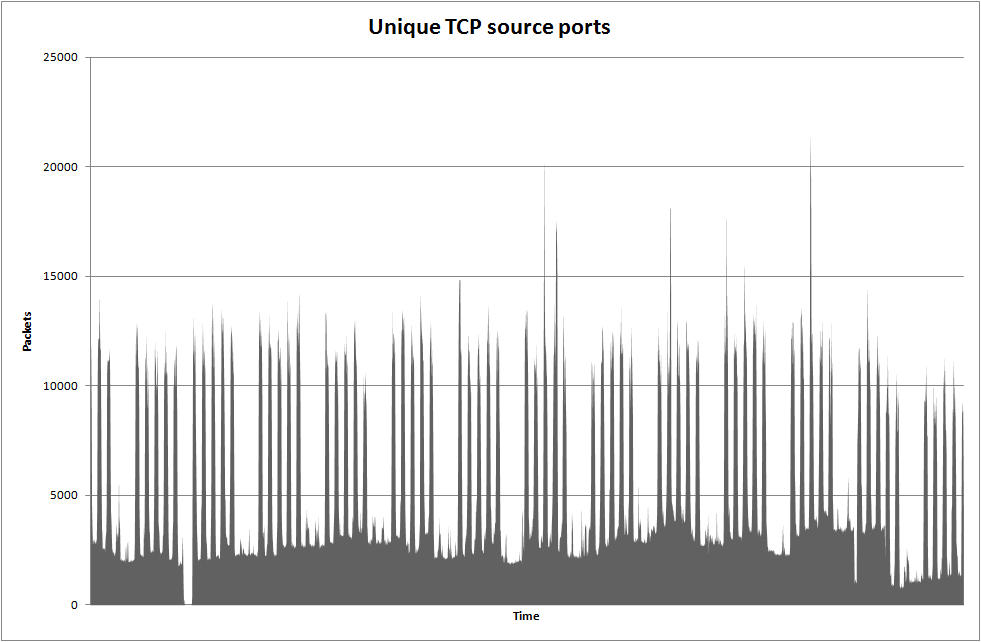
\includegraphics[width=0.5\textwidth]{tcp_src.png}}
\subfloat[Unique \emph{TCP} destination ports]{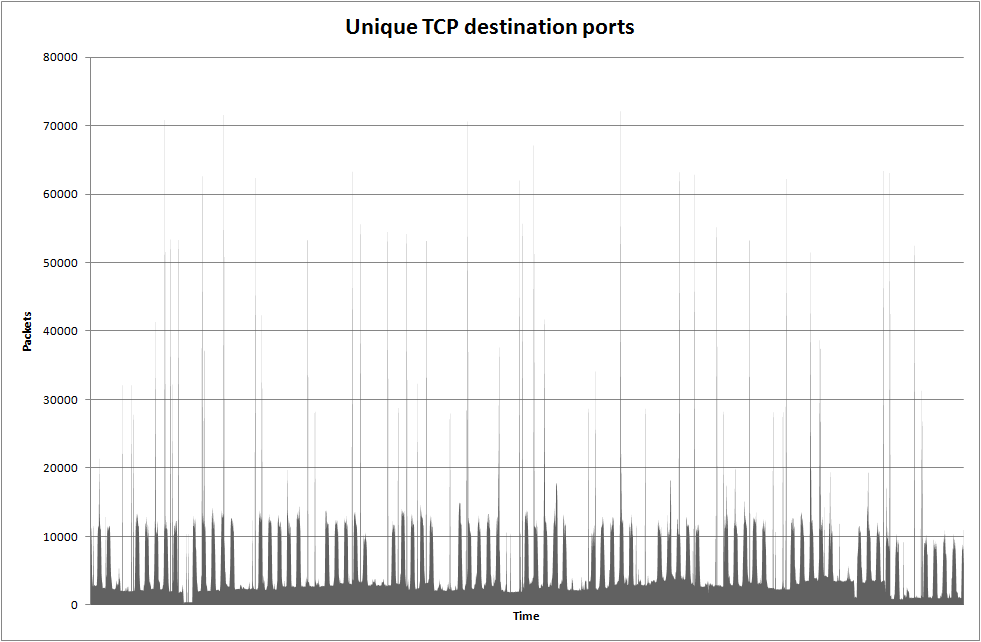
\includegraphics[width=0.5\textwidth]{tcp_dst.png}}
\\
\subfloat[\emph{TCP} connection attempts]{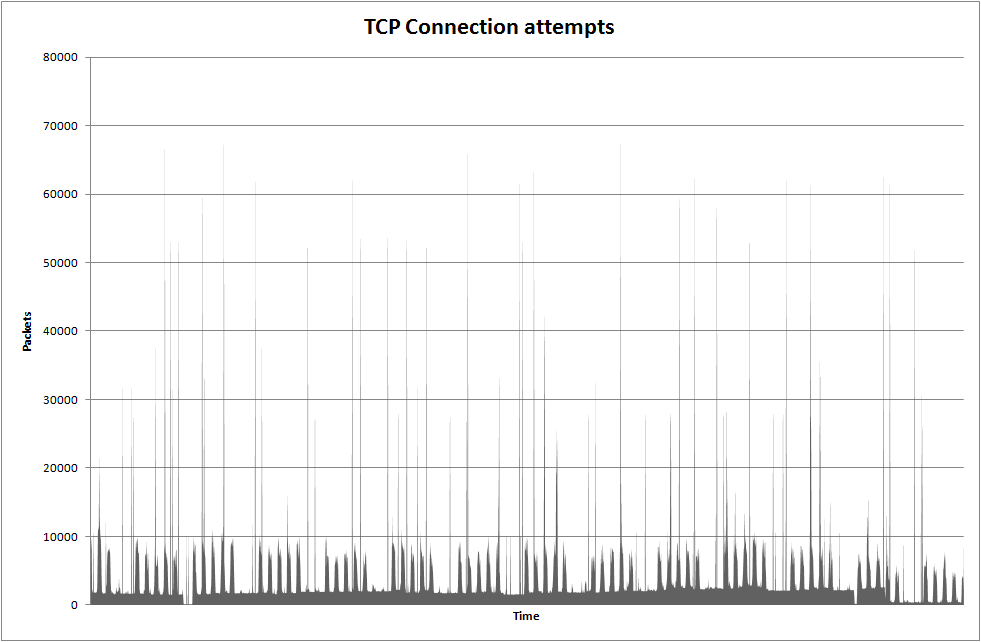
\includegraphics[width=0.5\textwidth]{tcp_attempts.png}}
\subfloat[\emph{TCP} connection count]{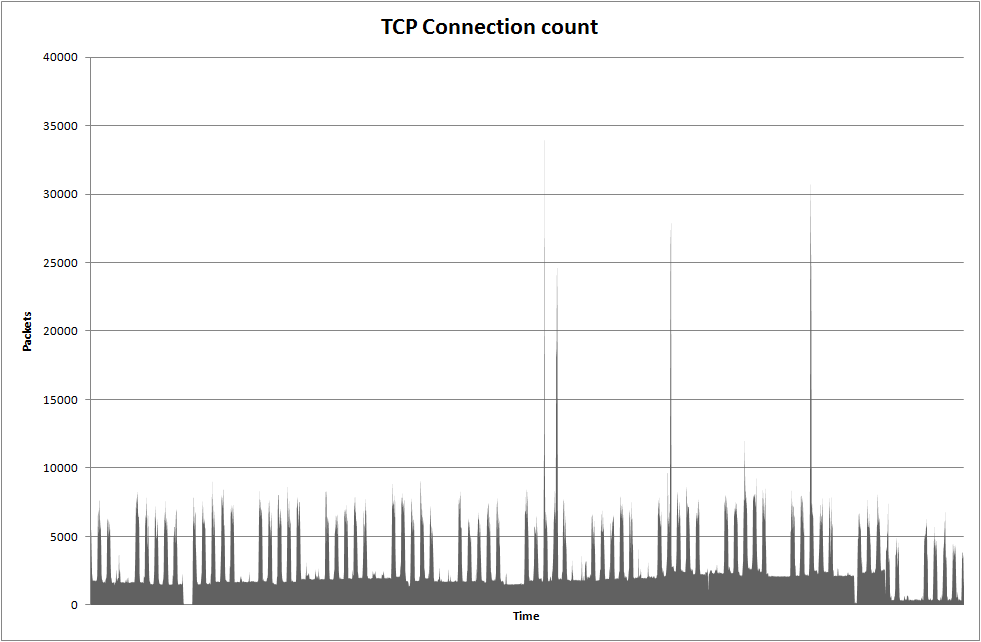
\includegraphics[width=0.5\textwidth]{tcp_connections.png}}
\caption[Vertical scan - entire data set]{Vertical scan - entire version of the data set. This time the divided version is omitted for brevity}
\end{figure}

Again, we run the anomaly detector against the modified data. The results are shown in table \ref{tab-scan}:

\begin{center}
\begin{table}
\centering
\begin{tabular}{l|l|l|l|p{1.5cm}|p{1.5cm}|p{1.5cm}}
\hline
\hline
\multicolumn{7}{c}{Clustering results} \\
\hline
Algorithm & data set & Preprocessing & Distance & True positives & False positives & False Negatives \\
\hline
\emph{K-Means++} & Entire & Z-Score & Euclidean & 33 & 201 & 67 \\
\emph{K-Means++} & Entire & - & Mahalanobis & 46 & 230 & 54 \\
\emph{K-Means++} & Divided & Z-Score & Euclidean & 68 & 140 & 32 \\
\emph{K-Means++} & Divided & - & Mahalanobis & 74 & 180 & 26 \\
\emph{DBSCAN} & Entire & Z-Score & Euclidean & 67 & 43 & 33 \\
\emph{DBSCAN} & Entire & - & Mahalanobis & 82 & 57 & 18 \\
\hline
\hline
\end{tabular}
\caption[Vertical scan - detected anomalies]{Detected anomalies for various combinations of clustering algorithms and distances. In total, 100 anomalies are injected in the original data set}
\label{tab-scan}
\end{table}
\end{center}

\subsection{Third example: protocol distribution alteration}

In this test, we no longer try to detect security-related anomalies, but a simple \emph{Network protocols distribution} measure is used.
This metric, as already mentioned before, consists of about twenty dimensions, each representing the evolution over time of a specific network protocol.
In this case, the anomaly detector is configured to export the statistics related to the following protocols: \emph{ARP}, \emph{Database}, \emph{Data transfer}, \emph{DHCP}, \emph{DNS}, \emph{SMTP/POP3/IMAP}, \emph{ICMP}, \emph{IPv6}, \emph{Microsoft networking}, \emph{Non IP}, \emph{Remote Desktop}, \emph{Routing}, \emph{SNMP}, \emph{SSH}, \emph{Voice/Video}, \emph{VPN}, \emph{Web}, \emph{Unknown}.

The injected anomalies mainly correspond to traffic changes generated by artificially replicating a multitude of packets of the same protocol over a rather small (and variable) time interval.
The intensity of these outliers is extremely variable, in order to better reflect a hypothetical real situation.
In addition, some anomalies are simultaneously injected for multiple protocols (e.g. to simulate an overload of a link or a malfunction of the network).

The total number of injected faults is, again, 100.

Although simple, this is the first test where we have a high-dimensional data space (20 dimensions), and so the \emph{PCA} technique has been heavily used as pre processing step for all the combinations of algorithms.
We tried several combinations of dimensionality reduction in order to preserve the greatest amount of information (in terms of detection rate), trying to avoid the effects of the curse of dimensionality problem, and the results are summarized in table \ref{tab-proto}.

\begin{center}
\begin{table}
\centering
\begin{tabular}{l|l|l|l|p{1.5cm}|p{1.5cm}|p{1.5cm}}
\hline
\hline
\multicolumn{7}{c}{Clustering results} \\
\hline
Algorithm & data set & Preprocessing & Distance & True positives & False positives & False Negatives \\
\hline
\emph{K-Means++} & Divided & - & Mahalanobis & 7 & 236 & 93 \\
\emph{K-Means++} & Divided & PCA & Mahalanobis & 18 & 193 & 82 \\
\emph{DBSCAN} & Entire & - & Mahalanobis & 10 & 158 & 90 \\
\emph{DBSCAN} & Entire & PCA & Mahalanobis & 23 & 111 & 77 \\
\hline
\hline
\end{tabular}
\caption[Network protocols distribution - detected anomalies]{Detected anomalies for various combinations of clustering algorithms and distances with and without using PCA. When PCA is used, the multi dimensional space is reduced to 8 dimensions (20 in the original data set) In total, 100 anomalies are injected in the original data set}
\label{tab-proto}
\end{table}
\end{center}

As it possible to see, in this scenario the clustering algorithms behave much worse than before (with a very high number of false alarms), where the dimensions of analysis were substantially small.
In this case, clustering can only detect anomalies involving multiple protocols: obviously this is an interesting point but, from our point of view, using this type of semantically-rich metrics, it would be useful as well to considered each dimension independently, for example by following each protocol trend independently, detecting the anomalies based on the specific pattern of each metric (e.g. weekly periodicity, etc.).

\subsection{Comparison with a single dimension analysis}

Although these simple results demonstrate that the use of clustering algorithms is quite effective only in detecting the types of anomalies that simultaneously affect more dimensions \footnote{It is not excluded that there exist other clustering-based approaches that, using more complex mathematical tools, get better results. In this research we tried to see what happens when using a simple and light, from a computationally point of view, approach.} (especially when introducing more complex algorithms such as \emph{DBSCAN} and distance measurements based on  the statistical dependence between the involved variables such as the Mahalanobis distance), it is even interesting to notice that this type of anomalies could be detected simply by considering each dimension independently, and possibly correlating the results later, as a post processing step.
For example, if we consider a really trivial kind of analysis, like calculating a threshold, based on standard deviation, above which the points are identified as outliers, we obtain, for the dimension \emph{ICMP} packets in the first test (the distributed bandwidth flood):

\begin{table}
\centering
\begin{tabular}{l|l|l|l}
\hline
\hline
\multicolumn{4}{c}{Results based on threshold} \\
\hline
Threshold & True positives & False positives & False Negatives \\
\hline
1$\sigma$ & 100 & 12 & 0 \\
2$\sigma$ & 77 & 0 & 23 \\
\hline
\hline
\end{tabular}
\caption[Bandwidth flood - detected anomalies using standard deviation]{Detected anomalies using a simple standard deviation-based comparison. In total, 100 anomalies are injected in the original data set}
\end{table}

\begin{figure}
  \centering
  \subfloat[\emph{ICMP} with 1$\sigma$ threshold]{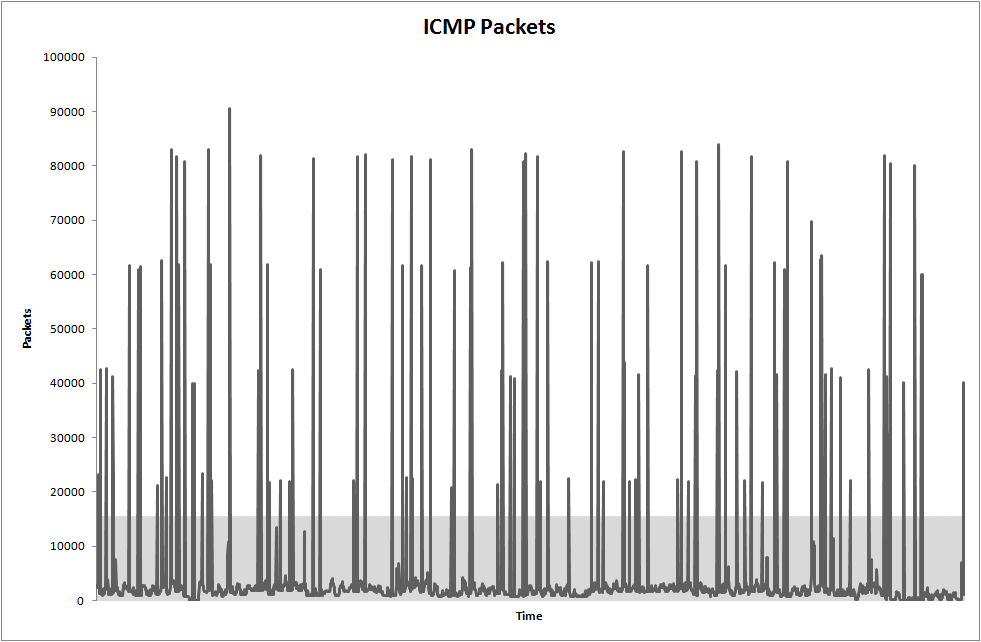
\includegraphics[width=0.5\textwidth]{icmp1stddev.png}}
  \subfloat[\emph{ICMP} with 2$\sigma$ threshold]{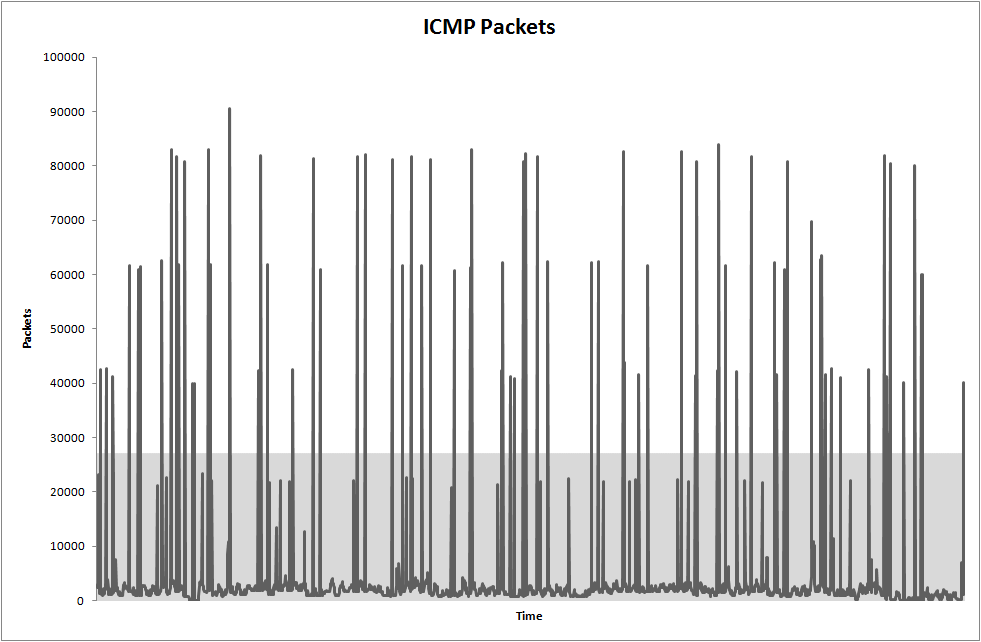
\includegraphics[width=0.5\textwidth]{icmp2stddev.png}}
  \caption{\emph{ICMP} Packets with standard deviation threshold}
\end{figure}

And we could do the same with the other dimensions, correlating later the results obtained.

Of course this method would not be so effective in the detection of more hidden anomalies (such as those that does not cause major changes in traffic), because in that case it would be wiser to consider more variables simultaneously, like in the clustering approach. 
Despite this, the main problem is that, increasing the number of dimensions, the results of clustering become more sensitive to the curse of dimensionality problem, and the output is severely compromised (if we add further dimensions to the previous example, surely we would get worse results).

\chapter{Discovering network anomalies using a time series analysis approach}

This chapter explains another model for anomaly detection, whose engine is no longer based on a clustering algorithm, but uses methods for analyzing time series data in order to extract meaningful statistics and other relevant characteristics.

The premises are the same of the previous model, as the metrics to be investigated are still really interesting, regardless the used model, and they represent a quite original data set for detecting network anomalies (and so the list presented in the previous section remains valid), and also the interface with the capture engine remains the same.

\section{Introducing \textit{Hey}, the \textit{human eye-like} algorithm for outliers detection}

We tried another approach because basically we wanted to solve some of the problems encountered during the testing of the clustering-based model. Some of these main issues are therefore:

\begin{itemize}
\item \textbf{Problems with high dimensionality data}: as it has been pointed out repeatedly, the results of a clustering algorithm are severely compromised when the number of dimensions in the data set is large. As it is possible to see from the previous tests, this problem can be partially solved using a preprocessing step as the \emph{Principal Component Analysis} method, or some distance measures more complex than the ordinary Euclidean distance, but, in any case, this issue still exists and it is inherent in the kind of analysis that clustering performs on the data.
For example, in some tests clustering behaves quite well, because the number of considered dimensions is relatively small. 
Another test was performed using a single metric, \emph{Network protocol distribution}. In this specific case, the capture engine exports about twenty time series to the anomaly detector, each one representing the trend over time for one of the twenty most widely used protocols in the network, in terms of bandwidth. Even using the most complex options available in our designed model, the clustering algorithm failed to detect some obvious anomalies, like a huge spike of \emph{SSH} traffic (200 times over the normal pattern) which lasted for several hours. This is because all the other nineteen dimensions were totally in the normal range, and then calculating the distance in a high dimensional space leveled the spike. Contrarily, from the point of view of a network administrator, these kind of anomalies are really interesting indeed;

\item \textbf{Effectiveness of using an algorithm with ``a priori correlation''}: using cluster analysis, most metrics are tied together in a multi-dimensional space. Since this is done before the algorithm runs, essentially this means that the detected anomalies must involve all the measures we are observing. But is it exactly what we want and what we expect? A strategy like this works extremely well when the analyzed metrics are simple and, taken individually, essentially worthless (as in the previous test, in which metrics were simply measures of dispersion for the most basic fields of \emph{TCP} and \emph{UDP} protocols). But when the metrics contain more meaningful informations from a semantic point of view, it would be more appropriate to analyze anomalies independently for each metric, possibly correlating the results during a second step. Exploiting this principle, the new proposed model for doing network anomaly detection becomes substantially more scalable and can work simultaneously with many time series, also completely heterogeneous between them (basically there is no more an upper limit). Without correlation, it is possible to simultaneously monitor very different metrics, such as volume-related metrics and performance-related metrics. This is a pretty good approach in order to control the overall ``health status'' of a network;

\item \textbf{The importance of time dimension}: as it was mentioned earlier, the data coming from the capture engine are essentially time series, formally defined as sequences of data points measured at successive times spaced at uniform time intervals, and therefore the information to be considered is basically the couple ``time point'' and ``value''. Using cluster analysis, this information is essentially lost, because all points are equally considered, independently from the time interval in which the values are captured. By exploiting the empirical observation that most of the metrics analyzed show a strong periodic component (mainly on a daily and weekly basis), we tried to ``force'' the clustering algorithm by splitting the entire data set into data blocks in which we put the samples collected from the same time intervals (and then running a separate instance of the clustering algorithm for each data block), but this thing only works partially and it is not generic nor precise. The new proposed approach is heavily based on this consideration, and the ``time'' variable becomes extremely important;

\item \textbf{Possibility of doing a reactive online anomaly detector}: Clustering is not well suited to perform on line anomaly detection, mainly for computational reasons \footnote{The complexity of the tested algorithms is given in the previous chapter. However, in our implementation, we tried several sizes of the data set and, for example, using an historical data set of 6 months with a sampling time of 10 minutes, it took about one minute for the K-Means++ to execute, and few minutes for the DBSCAN. From our point of view, this is really too much because an algorithm like that would fail to perform well on network devices like routers or capture probes. This issue could be solved by collecting all the data in a central elaboration unit, with enough computational resources, but this is beyond the purposes of this document.}. The new proposed model requires low computational resources, and so it is possible to detect anomalies in real time (by real time we mean that we can determine in a relatively short time if a new sample, which represents a snapshot of the network metrics caught at a regular sampling time, is an anomaly or not;

\end{itemize}

So, basically every metric in this approach is analyzed independently and treated as a completely isolated time series. The idea behind, rather simple and empirical, is to calculate, on the basis of the available historical data, some useful information in order to ``predict'' how the signal behaves in the future. This information is compared with each new sample to determine whether it is an anomaly or not.
In general, the proposed algorithm tries to trace what the human eye would notice having the charts showing the metrics plotted over time.
For the network-related metrics, the anomalies we are looking for are basically:

\begin{itemize}

\item \textbf{Short and impulsive changes}: basically this means \emph{peaks}. Peaks indicate significant events such as sudden increase or decrease of the metric for a limited amount of time (e.g. bursts in data traffic, etc.). 
It is very easy for the human eye to visually identify peaks in a univariate time series, but there is a need to formalize the notion of a this event to avoid subjectivity and to devise algorithms to automatically detect peaks in any given time series.
We can say that a data point in a time series is a local peak if it is a large and locally maximum value within a window, which is not necessarily large nor globally maximum in the entire time-series. Moreover, it must be isolated, i.e. not too many points in the window have similar values. 
Not all local peaks are true peaks; a local peak is a true peak if it is a reasonably large value even in the global context.
We will use these definitions to develop simple heuristics to detect such changes;

%figura picco con 2 o 3 settimane

\item \textbf{Long and persistent changes}: these anomalies are less impulsive and intense than the previous ones, and essentially can be defined as variations of the typical signal pattern that go on for a long period of time. For example, a variation of the bandwidth usage (let's say a fifty percent increment) which lasts for an entire night during a Sunday is a typical example of this type of anomaly;

%figura trend variation con 2 o 3 settimane

\end{itemize}

% elenco degli step
% schema a blocchi
The basic steps of the proposed model are then:

\begin{enumerate}
\item \textbf{Data acquisition}: as in the previous model, the network metrics are acquired using the capture engine, which exports them as discrete-time signals, with a customized time aggregation interval;
\item \textbf{Periodicity discover}: since many of the analyzed signals show a strong periodic component, it is extremely necessary to determine the correct periodicity, if any, using a sufficiently strong algorithm to neutralize the noise effect, which is inevitably present;
\item \textbf{Baseline computation}: for each signal, it is then necessary to calculate the baseline, which is the expected shape of the time series over the estimated period, on the basis of the historical data available;
\item \textbf{Short-term outlier detection}: this phase essentially coincides with the determination of the peaks, and a simple algorithm is used, based on the formal definition of peak for a time series;
\item \textbf{Long-term outlier detection}: in this last step, long-term abnormalities are detected using an algorithm based on a set of moving averages that attempts to highlight the pattern changes for a particular metric;
\end{enumerate}

In the rest of this section, each of these points is explained in depth.

\section{Data acquisition}

There is not much more to say about the data acquisition step, since a lot of things have already been said in the previous chapter and some implementation details will be given in the next chapter.
In any case, it is important to note that at this step we must choose the time aggregation interval we want to use to capture the network metrics.

In this case, the choice is totally arbitrary: in fact, in the first model, the computational limits of clustering algorithms prevented us from capturing the points too quickly over time, because otherwise the cardinality of the data set grew too much and the time required for processing became untenable for a scenario in which we want to execute the anomaly detection engine anomaly detection directly on the network probe that captures the data (as explained before). With this new very simple and lightweight model, instead, we do not have any limits on this parameter, but we have to specify this value in advance. This largely depends on which kind of network metric we are considering, and the reactiveness we want from our algorithm (because, if we choose smaller aggregation interval of aggregation, the model will be more responsive but we will also get more false alarms).
The following figures contains some examples of the same metric sampled with different time intervals, and it is quite evident that the shape of the signal varies depending on the chosen value (and so, the detected anomalies will be probably different as well).

\begin{figure}
\centering
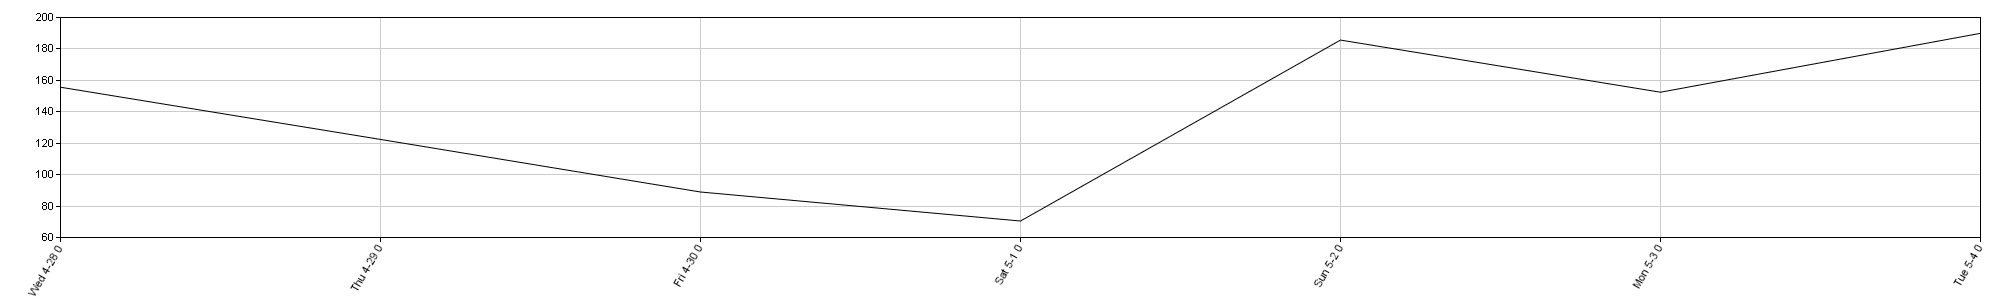
\includegraphics[width=\textwidth]{bw1day.png}
\caption{Bandwidth analysis for a week of traffic - Time aggregation interval: 1 day}
\end{figure}

\begin{figure}
\centering
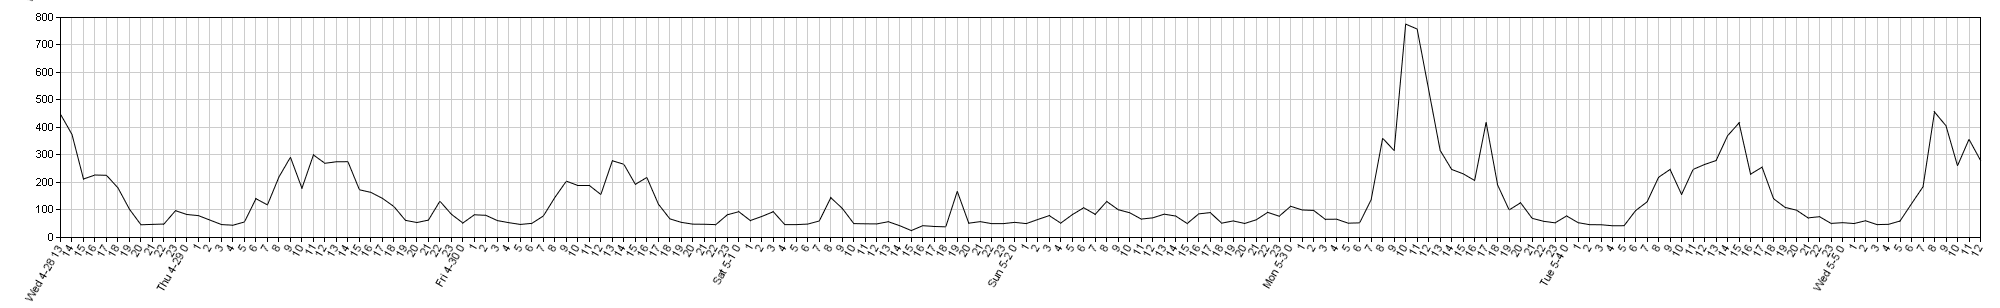
\includegraphics[width=\textwidth]{bw1hour.png}
\caption{Bandwidth analysis for a week of traffic - Time aggregation interval: 1 hour}
\end{figure}

\begin{figure}
\centering
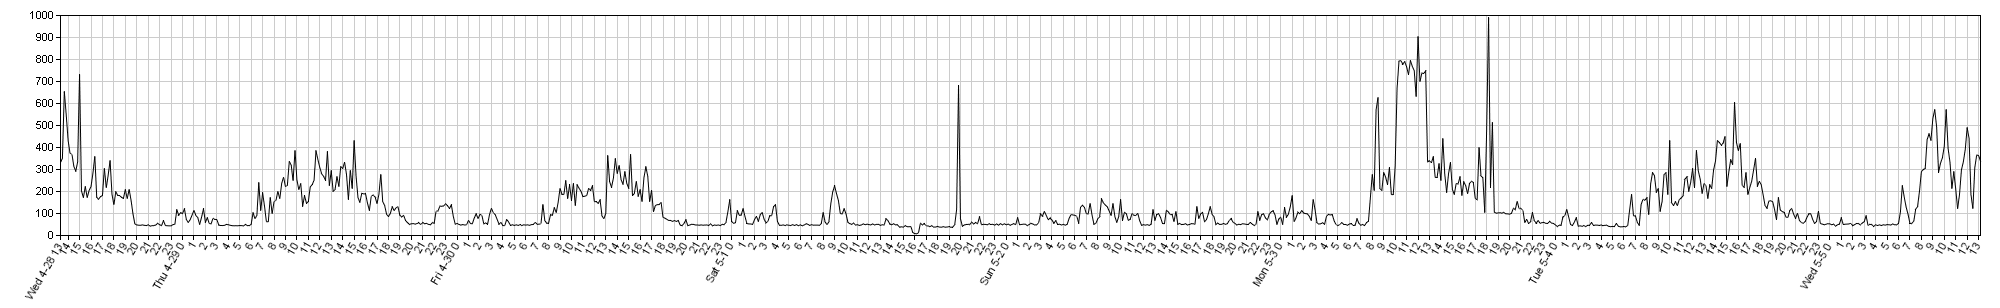
\includegraphics[width=\textwidth]{bw10min.png}
\caption{Bandwidth analysis for a week of traffic - Time aggregation interval: 10 minutes}
\end{figure}

\begin{figure}
\centering
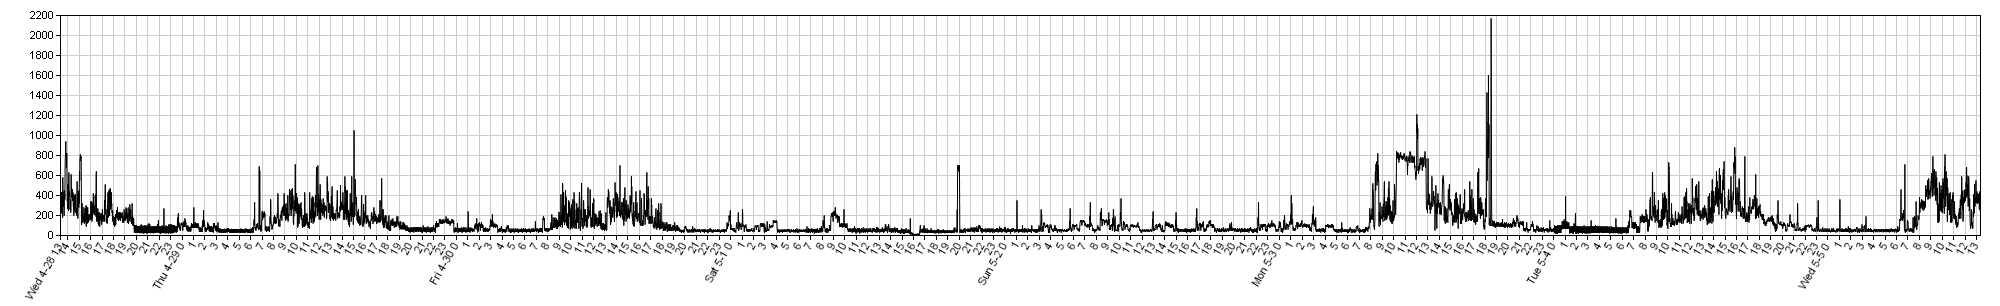
\includegraphics[width=\textwidth]{bw1min.png}
\caption{Bandwidth analysis for a week of traffic - Time aggregation interval: 1 minute}
\end{figure}

It is clear that certain types of anomalies are evident only when using a smaller aggregation interval, so the choice, as said before, heavily depends on the type of outliers we want to detect.

In general, during our tests, we found that a good compromise which works reasonably well with all the metrics we considered is achieved when the aggregation interval is set to ten minutes, and then we have always used this value, estimated empirically.
However, nothing prevents us to change this, since the logic of the algorithm does not depend on this parameter.
Although this option has not been proven, we can also think to use several instances of the algorithm, which are executed in parallel on the same network metrics sampled at different time intervals.

\section{Discovering periodicity}

The first essential step for this method is to discover the periodicity of the input data.
Since, as pointed out earlier, each metric is considered in a totally independent way, this estimate must be made for each time analyzed series.
This allows us to simultaneously work with completely heterogeneous metrics: for example, the typical ``bandwidth over time'' has a strong weekly period, while the ``\emph{IP TTL} distribution'' is essentially constant over time unless there are some problems in the network (which should be recognized and reported as anomalies).
Unfortunately, a simple answer to this problem does not exist. Period detection in time series can be complicated, and asking for an automated routine that can perform magic is too much.
Assuming we are interested in a robust way to discover the periodicity of a generic time series affected by a lot of noise (like our metrics, because they are based on data from the real world, and then the interesting patterns are often hidden in noise), there are basically two types of strategies to to deal with this issue:

\begin{itemize}
\item \textbf{Spectral strategy}: one approach is to find the frequency corresponding to the maximum of the spectral density. However, the spectrum at low frequencies will be affected by the amount of noise in the time series, making it difficult to distinguish. There are some techniques for resolving this problem, but they are rather complex and computationally expensive;

\item \textbf{Autocorrelation strategy}: basically, a robust autocorrelation estimate is computed and analyzed in order to find repeating patterns for the time series;
\end{itemize}

For our model, we choose an autocorrelation-based algorithm, since it seems to be quite robust with the presence of noise. 
In the following, a formal presentation of the algorithm is illustrated.

\subsection{Autocorrelation and autocorrelation plot}

Autocorrelation is the cross-correlation of a signal with itself. 
It can be seen as a similarity measure between observations as a function of the time separation between them. 
It is a mathematical tool for finding repeating patterns, such as the presence of a periodic signal which has been buried under noise, or identifying the missing fundamental frequency (strictly related to the periodicity) in a signal implied by its harmonic frequencies. 
It is often used in signal processing for analyzing functions or series of values, such as time domain signals.
More generally speaking, the autocorrelation function is extremely useful for:
\begin{itemize}
\item Detecting \emph{non-randomness} in data;
\item Detecting whether an observation is \emph{related} to other observation (at different time intervals);
\item Detecting an \emph{appropriate model} for the observed signal;
\end{itemize}

In our case, we use an approach based on autocorrelation, instead of a more classical spectrum-based method (like \emph{Fourier} or \emph{Wavelet} transform), in order to discover the periodicity of a time series, which is a really important information for detecting anomalies in an univariate signal.

From a mathematical point of view, if we consider a time series having sequential samples across time like $Y_1$, $Y_2$, etc., $Y_N$, the autocorrelation function at lag $k$ is defined as:

\begin{center}
\Large
$r_k = \frac{\sum_{i=1}^{N-k}{(Y_i - \overline{Y})(Y_{i+k} - \overline{Y})}}{\sum_{i=1}^{N}{(Y_i - \overline{Y})^2}}$
\end{center}

The time variable is not used in the formula for autocorrelation, since we assume that the observations are equi-spaced (no gaps between samples).
In this sense, autocorrelation is a correlation coefficient. However, instead of correlation between two different variables, the correlation is between two values of the same variable at times $X_i$ and $X_{i+k}$.

When the autocorrelation is used to detect non-randomness, it is usually only the first (lag 1) autocorrelation that is of interest (because in that case we only need to discover whether two sequential observations are related or not).
When the autocorrelation is used to identify an appropriate model for the analyzed signal (our case), the autocorrelations are usually computed for many lags.
Following this idea, we can create an autocorrelation plot (also known as correlation plot or \emph{correlogram}): on the horizontal axis, we put the time lag $h$ ($h$ = 1, 2, 3, etc.), while on the vertical axis we put the autocorrelation coefficient, calculated as:

\begin{center}
\Large
$R_h = C_h/C_0$
\end{center}

where $C_h$ is the autocovariance function:

\begin{center}
\Large
$C_h = \frac{1}{N}\sum_{t=1}^{N-h}{(Y_t - \overline{Y})(Y_{t+h} - \overline{Y})}$
\end{center}

and $C_0$ is the variance function:

\begin{center}
\Large
$C_0 = \frac{\sum_{t=1}^{N}{(Y_t - \overline{Y})^2}}{N}$
\end{center}

Having the autocorrelation plot, it is possible to use it to analyze key features of data.

If the time series contains a periodic pattern, then the correlogram also exhibits an oscillation at the same frequency.
Although the periodic behavior might be detected by the human eye without any major complications directly observing the original signal, the correlogram shows much more cleaner data and it is possible to launch a simple and automated algorithm which detects where the peaks of the curve are located (in terms of lags), and if these are multiple among them, the period is automatically determined.

If a residual series is random, then for large $N$, approximately 95\% of the values should lie in the range $\left [-2/N, 2/N\right ]$, and it is possible to plot two horizontal lines: the interval between them is a 95\% confidence band. 
A more exact procedure can be achieved by using t-statistics values for each autocorrelation.
The most important thing to notice is when we have a lot of values outside this confidence interval: in this scenario, we can assume the data is basically non-random, and then it is possible to analyze with more details the autocorrelation plot and start looking for a periodicity in the original signal.

\begin{lstlisting}[frame=shadowbox,caption=Algorithm for periodicity estimation using autocorrelation,language=C,tabsize=2,basicstyle=\scriptsize]
// Compute the correlogram from the data
correlogram(data)

// This provide a good estimation of the threshold
threshold = 1.96 / sqrt(data size)

for (every point in the data set)
{
	// If the current point is positive
	if (point > 0)
	{
		// If the curve is growing
		if (growing)
		{
			// If the curve is inverting the trend
			if (point < previous point)
			{
				growing = false

				// We reached a peak
				// Check if this is a valid maximum
				if (valid maximum)
				{
					save the new period
				}
			}
		}
		else
		{
			// If the curve starts to grow
			if (start growing)
			{
				growing = true
			}
		}
	}
}
return period
\end{lstlisting}

As an example, we can see three real network measures: a bandwidth measure captured with daily aggregation (figure \ref{img:correlogram_bw1}), another bandwidth measure captured with hourly aggregation (figure \ref{img:correlogram_bw2}) and a measure of the average \emph{TCP} round trip time for every connection captured with daily aggregation (figure \ref{img:correlogram_rtt}). These measures cover a period of four months, and, as we can see, the plots exhibit an alternating sequence of spikes. Such a pattern is the autocorrelation plot signature of a periodic behavior, and it is very easy to write an algorithm to calculate the distance between the peaks.

\begin{figure}
\centering
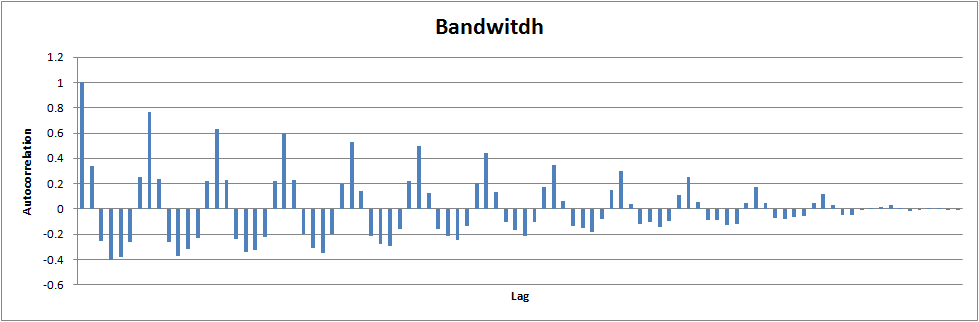
\includegraphics[width=\linewidth]{correlogram_bw1_2.png}
\caption[Correlogram for a bandwidth measure (daily aggregation)]{Correlogram for a bandwidth measure (daily aggregation). Each bar of the chart shows the correlation of a day with another day of the historical set. The empirical algorithm identifies the period 7 days.}
\label{img:correlogram_bw1}
\end{figure}

\begin{figure}
\centering
\includegraphics[width=\linewidth]{correlogram_bw2_2.png}
\caption[Correlogram for a bandwidth measure (hourly aggregation)]{Correlogram for a bandwidth measure (hourly aggregation). Each bar of the chart shows the correlation of a hour with another hour of the historical set. The empirical algorithm identify the period 24 hours.}
\label{img:correlogram_bw2}
\end{figure}

\begin{figure}
\centering
\includegraphics[width=\linewidth]{correlogram_rtt_2.png}
\caption[Correlogram for an average \emph{TCP} RTT over time (daily aggregation)]{Correlogram for an average \emph{TCP} RTT over time (daily aggregation). Each bar of the chart shows the correlation of a day with another day of the historical set. The empirical algorithm identify the period 7 days.}
\label{img:correlogram_rtt}
\end{figure}

Another example to show how the plot behaves analyzing non-periodic data is obtained observing the dynamics of ARP traffic (figure \ref{img:correlogram_arp}): the frequency of these types of packets is fairly constant in a common network, and do not strongly depend on the user activity; then, analyzing the correlogram of a daily time series, the algorithm can not identify the peaks at regular time intervals.
The plot starts with a high autocorrelation at lag 1 (only slightly less than 1) that slowly declines. It continues decreasing until it becomes negative and starts showing an increasing negative autocorrelation. The decreasing autocorrelation is generally linear with little noise. Such a pattern is the autocorrelation plot signature of ``strong autocorrelation'', which in turn provides high predictability, but there is no explicit periodicity.

\begin{figure}
\centering
\includegraphics[width=\linewidth]{correlogram_arp_2.png}
\caption[Correlogram for the ARP traffic (daily aggregation)]{Correlogram for the ARP traffic (daily aggregation). Each bar of the chart shows the correlation of a day with another day of the historical set. The empirical algorithm does not identify any period for this signal.}
\label{img:correlogram_arp}
\end{figure}

\section{Creating the baseline}

After detecting the periodicity of the signal (and obviously this can not happen immediately, because with the autocorrelation-based approach at least two periods of historical data are needed, although it is possible to manually set the period, if it is already known for a certain metric), the basic idea is to build the baseline for that metric over the whole period (this is a rather popular idea, which can be found in many other anomaly detection models, including the non-network related ones\cite{wsare}).
Basically, at this stage we have all the historical data for a particular metric, so the easiest thing to do is to build the baseline as the weighted average of past samples.
A weighted average is used in order to give more importance to recent samples, so that the algorithm is more responsive when the pattern for that metric is changing.
The baseline for a given point within the period is calculated using the past samples in the neighborhood of that point, using a variable-width time window. This allows to smooth the signal, reducing the negative effects in case of noise.

Basically, the output of this step is a synthetic signal, whose length is equal to the previously estimated period, containing the expected values for the future samples, calculated on the basis of the historical available data.

More formally, the steps for estimating the baseline can be summarized as

%chart ppt 

\begin{enumerate}
\item Detect the period for the time series $x$, $p$;
\item Split the original time series $x$ into smaller signals $x_1, x_2, x_n$, each one having the length of the period $p$; 
\item Create a synthetic signal $b$ of length $p$. $b$ will contain the baseline data;
\item Populate the $b$ signal using a linear weighted average of the past samples over a time window. Each sample $b_i$ will be computed as:

\begin{center}
\Large
$b_i = \sum_{j = 1}^{p}{\frac{w_j}{size}\sum_{k = - size/2}^{size/2}{x_{jk}}}$
\end{center}

where $size$ is the window length for smoothing, and $w_j$ is the linear weight for the historical period $j$.
\end{enumerate}

As a simple example, let's consider the typical scenario of a metric having a weekly periodicity, whose new samples are exported from the capture engine every 10 minutes. Overall, the baseline will be a time series of $24\times7\times6$ samples. Assuming that the size of the window for smoothing the signal is 1 hour, and assuming we also have 10 weeks of historical data, the baseline for the Monday at 8:30 is created by a linearly weighted average (e.g. samples from week 10 weighs 1, samples from week 9 weighs 2, etc.) of all the samples included in the historical data within the range between the Monday at 8:00 and the Monday at 9:00.

\begin{figure}
\centering
\includegraphics[width=\linewidth]{baseline.png}
\caption{Baseline computation}
\end{figure}

\section{Detecting outliers with simple heuristics}

After capturing for each metric a sufficient number of samples to estimate the period and compute the baseline for that signal, the outlier detection step can begin.
Basically, what we are doing is decomposing a time series into seasonal and irregular components using moving averages.
So, first we determine seasonal figure by averaging, for each time unit, over all periods within the smoothing window. 
Then, the error component is determined by removing this seasonal figure from the original time series.
The resulting time series contains the so called ``residuals''. 
The sequence of residuals ordered by time essentially represents another time series, which mainly contains noise and the outliers which we are looking for.
Unfortunately, in this specific field of application, the noise is not stationary, and it largely depends on the type of metrics we are using (e.g.  during the tests we noticed that the noise level for metrics that capture information about the volume of the traffic in a network is almost directly proportional to the absolute value of the signal at that point, while for performance-related metrics measuring like response times the noise is always basically constant, regardless of the signal).
To solve this problem it is extremely important to carefully choose thresholds used by the simple algorithms for detecting the two categories of anomalies listed above.

%grafico residui

In addition to the seasonal and irregular component, the decomposition of the original time series could also take into account a long-term trend.
This thing could be done for example by introducing an additional component of decomposition, based on a linear regression over all the historical values.
Since this represents another large problem, the proposed model (and the implementation used during the tests) is not paying attention to this issue, and the long-term pattern change for a metric is handled by simply discarding historical data older than a given value (depending on the metric this value may be one week, one month, six months, etc.).

\subsection{Detecting short-term anomalies}

Having the time series composed by the residuals of the original signal, the short-term anomalies can be identified essentially detecting the peaks of this new signal.
In fact, the peaks are quite evident even in the original metric (without carrying out the seasonality decomposition), but the advantage of working directly with the residuals is that, with that approach, a more ``locally'' stationary signal is expected, since the only factor which might create disturbance in the anomaly detection procedure is the noise (which unfortunately can be very annoying also working with this approach).

It may seem very trivial to detect this kind of outliers, especially because it is so obvious where they are to the human eye, but making a computer find them can turn out tricky.
Some of the most popular approaches which can be found in the literature to perform this detection are:

%picco

\begin{itemize}
\item Use a ``travel'' and ``rise'' approach to model the dynamic of a time series. Basically, between any two points in the signal, $(t_0,y_0)$ and $(x_n,y_n)$, add up $y_{i+1}-y_i$ for $0 <= i < n$ and call this $T$ (travel) and set $R$ (rise) to $y_n- y_0 + k$ using a suitable $k$. $T/R > 1$ indicates a peak. This is simple, but works quite well only if large travel due to noise is small or if noise is symmetrically distributed;

\item Use a \emph{zero-derivate} method. It exploits the principle that the first derivative of a signal changes sign when the trend reverses. Using appropriate threshold parameters, it is possible to define a peak as an ``abrupt'' change of the first derivative of the time series, from positive to negative values. This method is simple as well, but it is extremely sensible to the noise, which unfortunately is always present in real-life signals (and especially in network metrics), because a lot of accidental zero-crossings of the first derivate occur, yielding false detections. The typical solution is to smooth the curve with some low-pass filter;

\item Use a \emph{deconvolution} between a standard peak shape and the analyzed time series, and check for high values. Theoretically, this is a valid method, but, as it is possible to imagine, for a real signal it is extremely difficult to define a ``collection'' of peak shapes used to compare real samples;

\item Smooth the data and check for triplets of equally spaced points where, if $x_0 < x_1 < x_2$, then $y_1 > 0.5*(y_0+y_2)$, or check Euclidean distances like this: $D((x_0,y_0),(x_1,y_1)) + D((x_1,y_1),(x_2,y_2)) > D((x_0,y_0),(x_2,y_2))$, which relies on the triangle inequality.

\end{itemize}

Some of these methods (and indeed many others which were not mentioned) are valid only when applied to certain types of signals (for example, the deconvolution method is usually used with signals whose shapes vary in a limited way and the dynamics is well known, such as voice), while others (like the triplets-based method) are not sufficiently robust to be used in a scenario like ours, where the noise level is generally really high. A good survey about some of the most typical techniques for peak detection can be found in \cite{peak}.
In our case we wanted to try something new in order to solve the problem of working with a general and noisy signal.

The basic assumption is that, for the human eye, a peak is the highest point between ``valleys''.
What makes a peak is the fact that there are lower points around it. So, the strategy adopted by the implemented algorithm is to look for the highest point around which there are points lower by a certain threshold on both sides. The threshold is chosen according to the noise estimation of the residual component in the original time series.

\begin{lstlisting}[frame=shadowbox,caption=Algorithm for peak detection,language=C,tabsize=2,basicstyle=\scriptsize]
for (every residual point x[i])
{
	// Update minimum and maximum info
	if (x[i] > max)
	{
		max = x[i]
		max_pos = i
	}
	
	if (x[i] < min)
	{
		min = x[i]
		min_pos = i
	}
	
	if (look_for_maximum)
	{
		if (x[i] < max - threshold)
		{
			report a positive peak at time i
			min = x[i]
			min_pos = i
			look_for_maximum = false
		}
	}
	else
	{
		if (x[i] > min + threshold)
		{
			report a negative peak at time i
			max = x[i]
			max_pos = i
			look_for_maximum = true
		}
	}	
}
\end{lstlisting}

In the real implementation, the algorithm is more complex since some special cases are handled, like the presence of any gaps or the fact that if a peak is detected over a certain time limit, it is no longer reported as an anomaly (consistent with the assumption that this approach needs be as responsive as possible).

\subsection{Detecting long-term anomalies}

In addition to the detection of abrupt anomalies for a signal, another goal is to discover less intense anomalies which last longer over time (e.g. a pattern change for a metric). From an analytical point of view, these types of outliers are present in various forms and it can be particularly challenging to detect them in a real and very noisy signal.

%figura

The method proposed here is based, again, on empirical observations that were made during the tests for the clustering-based model. In general, what can be seen with the majority of network metrics is that these outliers are essentially temporary or permanent deviations of the pattern in the time series. An interesting example of one of these outliers which have been observed over real traffic during the tests was an increase of \emph{ARP} traffic: suddenly the ``network protocol distribution'' metric reported an increase for the \emph{ARP} traffic in terms of bandwidth, and this was constant over time. Later, it was discovered that the problem was caused by a badly configured \emph{load balancer}\footnote{\url{http://en.wikipedia.org/wiki/Load_balancing_(computing)}}.

To detect these deviations, it is again useful to work with the concept of ``residual'' of the signal. In this sense, considering the time series composed by the residuals only, such anomalies can be identified as the sequential samples whose value repeatedly exceeds, over time, the average of the residuals (for a signal with no abnormalities this should be simply equal to the noise average for that metric).

Since the average noise level for a generic network metric is usually too high, a simple mechanism based on thresholds such as ``if the residuals of the metric continuously exceed for two hours a certain threshold, then trigger an anomaly'' is not enough, and a slightly more robust approach is needed.
Again, it is very convenient to observe what the human eye would observe in front of a chart to determine this kind of abnormality. 

The basic steps are:

\begin{enumerate}

\item The periodic component is identified (if any);
\item The most obvious anomalies are detected, and they basically correspond to the intense peaks (already managed by the previous algorithm);
\item The less obvious anomalies are identified, and in most cases they are sequences of outliers repeated over time. The ease with which they are detected is proportional to the degree of deviation from the normal behavior and their duration in absolute time (e.g. a durable deviation from the pattern is easy to detect even if it is not very intense, while a shorter detour is easily recognizable only if more intense); 

\end{enumerate}

% disegno rettangolini

Exploiting this idea, another simple algorithm has been written and tested, and it works pretty well. Basically, every time a new sample is received from the capture engine, a set of moving averages is computed. Each moving average uses different values from the historical data, and each of them is compared with an appropriate threshold, which varies depending on the length of the moving average itself. In this way we try to do the same thing a human eye would do.

More formally, a parameter $maxavg$ is defined, which reveals how far the algorithm can go back in time to discover long-term anomalies (in our implementation a good estimate is 24 hours, since with this value it is possible to detect even a long pattern change keeping a low complexity). Basically, the algorithm proceeds by calculating $maxavg$ moving averages, each one having a size ranging from 1 to $n$ samples corresponding to the $maxavg$ time interval, going back from the current one. 
The result of each moving average is then compared with an appropriate threshold value.
The idea is to have an array of threshold values specifically created for this purpose. For example, the thresholds can be chosen with exponential weights, being much higher for the first values (which then correspond to the anomalies that do not last long, and therefore should be more intense in order to trigger an alarm), and significantly lower for the last (for moving averages which span over long time intervals, and so they can be globally less intense).

In this sense, the moving averages are used like finite impulse response filters to analyze the time series in order to smooth out short-term fluctuations and highlight longer-term trends or cycles (the anomalies, because the cycles are already subtracted since the averages are calculated using the residuals).

The algorithm can then be summarized as:

\begin{enumerate}
\item Define the parameters $maxavg$, $r$ (the array containing the residuals of the original metric), $thresholds$ (the array containing the thresholds for the moving averages);
\item Compute $maxavg$ moving averages of different sizes, starting from the residual estimated from the last sample. Basically, the moving average $i$ (if $maxavg$ is expressed as a multiple of the time interval used by the capture engine to emit new samples, $1 < i < maxavg$) is calculated as:

\begin{center}
\Large
$m_i = \frac{r_n + r_{n-1} + etc. + r_{n-i+1} + r_{n-i}}{i}$
\end{center}

\item Pick up the maximum value contained in the $m$ array, suppose $m_{max}$. This correspond to the time interval containing the past samples, including the last, which deviate more from the baseline;

\item If $m_{max} > thresholds_{max}$, the time period with length $max$ deviates enough to be considered a long-term outlier, and so it can be reported as an anomaly;
\end{enumerate}

By properly setting the $maxavg$ parameter and the $thresholds$ array, the detection procedure can be more or less reactive or sensitive.

\begin{figure}
\centering
\includegraphics[width=\linewidth]{movavg.png}
\caption[Moving average computation]{Moving average and dynamic threshold for short-term and long-term outlier detection. The image represents how the moving average-based algorithm works. The charts on the left show two examples of residuals, calculated by subtracting the expected baseline from the original signal. Then, using a window of variable size, a series of moving averages is computed. The two extremes of moving averages are a really short one and a really long one (e.g. some minutes vs some days). When the moving averages are computed (the blue vertical bars), they are compared with the thresholds (the red horizontal bars), whose level change according to the size of the moving average window itself. Following the paths indicated in the picture, the situation on top is identified as a short-term anomaly, while the signal at the bottom is identified as a long-term anomaly.}
\end{figure}

\subsection{Threshold selection}

After illustrating the algorithms, which were all created on the basis of simple empirical observations, the hardest part is to properly configure the parameters. 
As already seen with clustering, even in this model, the input parameters required by the algorithms are basically the time series to be analyzed and a general threshold value, which can be used in various ways (in the peak detection algorithm this value indicates the average difference between local minimum and maximum, while in the long-term algorithm it indicates the maximum allowed deviation of a moving average, with respect to the expected value).
Since network-related metrics come directly from the real world and therefore they are far from being perfect from a mathematical point of view, the most important factor that can significantly affect the results of any outlier detection algorithm is the noise, defined as any unwanted perturbation to a wanted signal, our time series. 
In order to reduce the bad effects of noise, it is required that the thresholds used by the algorithms are set over a certain values (substantially the noise level estimation for the residuals). The key question now is how to set the correct values to minimize false positives.

Exploiting the fact that, theoretically, if the signal was absolutely clean, the residuals should be completely stationary and with zero mean (without considering the anomalies), for the noise level estimation it is possible to use some popular concepts from the ``Robust statistics'' discipline.

Basically, what we want is a measure indicating the degree of dispersion of the residuals for a metric, from a local (within a window in the neighborhood of the points to be analyzed) and global (taking into account the dynamics of the signal during throughout its history) point of view.
This dispersion is then used as a multiplication factor for calculating the thresholds for each moving average.
Furthermore, this measure must be as simple as possible to calculate, in order to keep low computational requirements even when the algorithm needs to work with a large number of time series and a large amount of historical data (for example, a good anomaly detector for monitoring the health status of a network has to control several tens of metric, essentially all those illustrated in the previous chapter plus some other at the discretion of the network administrator who will configure the system).
Below, we show all the measures which have been taken into consideration, with advantages and disadvantages for each. Remember that each of these measures is computed using the time series composed by the residuals of the original signal. Each measure is calculated in two variants: first, using all the available samples, and then  using only the samples located within a local window (to estimate the local deviation).

\subsubsection{Standard deviation and mean absolute deviation}

\emph{Mean absolute deviation} and \emph{standard deviation} are two measures of dispersion or spread in a data set. 
They are commonly used as a summary of the range of scores associated with a measure of central tendency, the simple average.
The first is obtained by summing the squared values of the deviation of each sample from the mean, dividing by the total number of observations, and then taking the positive square root of the result, the second is equal to the average of the absolute differences between each sample and the overall mean. 
Considering with $X$ a univariate time series $X_1, X_2, etc., X_n$, the two formulas are:

\begin{center}
\Large
$Standard\;deviation = \sqrt{\frac{1}{N}\sum_{i=1}^{n}{(X_i - mean(X))^2}}$
\end{center}

\begin{center}
\Large
$Mean\;absolute\;deviation = \frac{1}{N}\sum_{i=1}^{n}{\left | X_i - mean(X)\right |}$
\end{center}

The main reason why the standard deviation was created like this is because the squaring eliminates all negative deviations, making the result easier to work with algebraically.
From a mathematically point of view, the mean deviation is preferable because is actually more efficient than the standard deviation in the realistic situation where some of the measurements are in error (a more formal explanation is given in \cite{stddev}); It is also more efficient for distributions other than perfect normal, and easier to understand (and this is particularly important since the algorithms described above are all based on empirical observations directly made during the tests).

The standard deviation is then reported only because it is an example of the best estimator if the underlying distribution is normal. However, it lacks robustness of validity. That is, confidence intervals based on the standard deviation tend to lack precision if the underlying distribution is in fact not normal.

\subsubsection{Median absolute deviation}

\emph{Median Absolute Deviation (MAD)} is another simple way to quantify the variation degree of a signal.
Half the values are closer to the median than the \emph{MAD}, and half are further away.
The best way to understand this measure is to understand how it is calculated. 
First, the median of all the set of values is computed (the median also represents the 50th percentile, a concept that is also used in the next presented measure).
Then, the distance between the values and the median is calculated.
Regardless of whether the resulting value is greater or less than the median, the absolute distance distance between it and the median is taken.
The last step is to find the median of that set of differences. The result is the \emph{MAD}.
In fact, there are two distinct computations of the median. First one computes the median of the actual data. Then one computes the median of the distances of the values from that median. 

The formula can be written as:

\begin{center}
\Large
$MAD = median_i = (\left | X_i - median_j(X_j) \right |)$
\end{center}

Where $X$ is a univariate time series $X_1, X_2, etc., X_n$.

This measure is resistant to outliers, because the presence of points having extreme values has limited effects on its actual value.

\subsubsection{Interquartile range}

The \emph{Interquartile Range (IQR)} is the last measure of statistical dispersion considered in this model, and it is equal to the difference between the third and first quartiles (where a quartile is any of the three values which divide the time series values, ordered, into four equal parts, so that each part represents one fourth of the sampled population) of a data set. 

A simple procedure for computing the interquartile range is:

\begin{enumerate}
\item Sort the samples $X$ in ascending order, so that $X_0 <= X_1 <= etc. <= X_n$;
\item Calculate $IQR$ as:
\begin{center}
\Large
$IQR = X_{round(0.75n)} - X_{round(0.25n)}$
\end{center}
\end{enumerate}

This way, we have simply computed the difference between the third quartile (which cuts off lowest 75\% of data) and the first quartile (which cuts off lowest 25\% of data). The second quartile is not used for the \emph{IQR}, but it is simply the median of the data, because it cuts the set in half.

The \emph{IQR} is pretty popular, since it is used as the basis of some simple statistical tools like the \emph{box plot}\footnote{\url{http://en.wikipedia.org/wiki/Box_plot}}, which is a convenient way of graphically visualize groups of data (such as time series) through five-number summaries: the \emph{smallest observation} (sample minimum), the \emph{lower quartile}, the \emph{median}, the \emph{upper quartile} and and the \emph{largest observation}. A box plot can easily indicate which observations might be considered outliers (for example, the original box plot's author said that points greater than one and a half interquartile ranges above or below the upper and lower quartiles are assumed outliers). 

%immagine box plot?

In our case, however, we do not use a tool like the box plot, since the \emph{IQR} is simply used to estimate the band of values that includes most of the residuals.

%citazione

The \emph{MAD} and the \emph{IQR} are estimates of dispersion that have robustness of validity, since they are effective even when the data contains outliers. Another great feature is that these measures does not make any assumptions of the underlying statistical distribution of the data set.

As an example of this, consider two hypothetical and very simple time series:

\begin{center}
$S_1 = \{10\;5\;7\;50\;34\;94\;113\;32\;201\;90\;10\;8\;44\;78\;64\;125\;39\;27\}$
\end{center}

\begin{center}
$S_2 = \{10\;5\;7\;50\;34\;94\;8462\;113\;32\;201\;90\;10\;8\;44\;78\;64\;125\;39\;27\}$
\end{center}

\begin{table}
\centering
\begin{tabular}{|c|c|c|c|c|}
\hline
\hline
Set & Standard deviation & Mean absolute deviation & MAD & IQR \\
\hline
$S_1$ & 52.05 & 40.45 & 32.5 & 41.5 \\
$S_2$ & 1928.84 & 838.14 & 34 & 44 \\
\hline
\hline
\end{tabular}
\caption{Comparison of different dispersion measures}
\end{table}

The time series $S_2$ contains the same values of $S_1$ (basically random data without imposing any statistical distribution) plus an evident outlier, added manually. 
Although the example is completely invented and artificial, this is a situation that can easily occur in a real signal (in the network metrics considered during the tests, these kind of particularly intense peaks are not rare), and generally an appropriate measure to determine whether they are part of the normal dynamics of the signal (e.g. in case of particularly impulsive traffic) or not is needed.
The example clearly confirms that standard deviation is the most sensitive measure to the presence of outliers, immediately followed by the mean absolute deviation, and hence they are the less appropriate for estimating the average dispersion for the residuals.
Despite these considerations, in literature the standard deviation is often chosen as a measure of dispersion for the outlier detection algorithms (in some cases the anomalies are identified as the samples above a certain amount with respect to the standard deviation \cite{stddev1}, while other approaches propose more complex procedures to reduce the noise sensitivity \cite{stddev2}).


Returning to the anomaly detector model, after choosing one of these measures of dispersion, the actual value is then calculated from all the historical data of the analyzed metric, and this is called $delta_{global}$.
Each time a new sample is received by the capture engine, a new measure of dispersion, $local_{delta}$, is calculated directly using the samples in the neighborhood of that new point (even from past periods, if necessary).
This is needed to introduce inside the algorithms the concept that an anomaly must be a change of pattern both globally and locally. Therefore, for each new sample $i$, the measure of dispersion is calculated as:

\begin{center}
\Large
$delta_i = w_{global}\,delta_{global} + w_{local}\,delta_{local}$
\end{center}

Where $w_{global}$ and $w_{local}$ are two weights by which it is possible to give more importance to one of the two deviations (whether the characteristics about the waveform of the metrics are not known, it is a good compromise to set this weights both to 0.5).

Finally, this value of $delta$ can be directly used by the two algorithms for detecting anomalies, because, for every moving average $m_i$ it is possible to compute the value $score_i$ as:

\begin{center}
\Large
$score_i = \frac{m_i}{delta_i}$
\end{center}

A moving average $i$ can be identified as an anomaly if its value $score_i$ exceeds a certain threshold. For choosing this threshold, it is possible to make one last trick: it might be interesting to introduce the concept of ``user threshold'', i.e. leave to an external user the possibility to calibrate the sensitivity of the algorithm using a simple parameter.
This can be done quite simply using the peak detection algorithm, since, assuming the user sets a $tolerance$ value, it is possible to use the value $delta \times tolerance$ as threshold, and the algorithm automatically finds more or less outliers depending on the value set.
For the long-term detection algorithm based on moving averages, instead, we have a whole array of thresholds, and the anomalies distributed over a longer time period require a lower threshold to be detected, following the example of what intuitively the human eye does in these cases.
To introduce this concept from the user-specified $tolerance$ value, it is possible to fill the $thresholds$ array using different weights which multiply the $delta$ value. For example, during the tests, a good compromise was reached using a formula like this:

\begin{center}
\Large
$threshold_i = (tolerance + \frac{(tolerance^2 - tolerance)}{1.1^{(i-1)}})$
\end{center}

\begin{figure}
\centering
\includegraphics[width=\linewidth]{threshold.png}
\caption[Dynamic thresholds]{Dynamic thresholds for a long-term detection algorithm having $maxavg$ = 72 (12 hours with a sampling time of 10 minutes) and $tolerance$ = 3.5. The shorter moving averages have a very high threshold (which decreases exponentially)}
\end{figure}

In this way, a very impulsive anomaly must be sufficiently intense in order to be detected, since an anomaly $i$ is triggered when $score_i > thresholds_i$.

\section{Validating the model}

Since the model was basically invented and constructed after a long series of empirical observations (the strategy adopted was to gradually improve a simple algorithm based on standard deviation and no periodicity, like the really trivial one introduced at the end of the previous chapter), it is rather difficult to give to the reader an objective methodology for validating the results.
The audits were in fact tests made by observing dozens of different metrics on real traffic traces, without any fake injection.
In the iterative process that led to the development of the proposed model, each incremental modification of the algorithm was tested on a certain number of metrics. For each detected anomaly, then, we examined the corresponding traffic, in order to observe if it was a real unexpected behavior or not (based on the considerations about what kind of outliers we would like to detect, as described in the previous sections). An example of the graphical output of the algorithm using some real metrics is given in appendix A.

Moreover, usually the anomaly detection works proposed in literature always refer to security-related anomalies; in this case, instead, the concept of anomaly becomes extremely larger, since any deviation from the expected behavior of a signal is detected, and therefore the evaluation criteria is in some way more subjective, and therefore delivering objective results is a really ambiguous task.

In any case, we tried to execute these algorithms on the same metrics considered in the previous chapter as well, when we validated the clustering model; Before proceeding, it is necessary to keep in mind the following observations:

\begin{itemize}
\item The anomalies injected are artificially generated and, as before, they are 100, but when considering each metric independently, we do not have 100 fake anomalies for each metric (e.g. during the ICMP-based bandwidth flood, the ``TCP packets'' metric is not affected by the injected anomalies);
\item All the other detected anomalies (beyond the 100 injected), in the table below, are labeled as false positives, and this, in the authors' opinion, is not particularly realistic, because in these cases it is easy to identify other obvious abnormalities in addition to the injected ones, but this approximative decision was taken in order to try to give more uniformity to the results of the two proposed approaches;
\item The following scenario is only a purely informative addition, and the obtained results did not influence the authors during the development of the algorithm, since the ideas underlying the model have been based only on what kind of anomalies was expected by manually looking at the metrics computed on real traffic;
\end{itemize}

\begin{center}
\begin{table}
\begin{tabular}{l|c|c|c}
\hline
\hline
\multicolumn{4}{c}{Distributed bandwidth flood - results} \\
\hline
Metric & True positives & False positives & False Negatives \\
\hline
ICMP packets & 89 & 5 & 11 \\
TCP packets & 0 & 21 & 0 \\
UDP packets & 0 & 13 & 0 \\
Unique IP source addresses & 95 & 9 & 5 \\
Unique IP destination addresses & 0 & 32 & 0 \\
\hline
\hline
\end{tabular}
\caption{Distributed Bandwidth flood - detected anomalies}
\end{table}
\end{center}

\begin{center}
\begin{table}
\begin{tabular}{l|c|c|c}
\hline
\hline
\multicolumn{4}{c}{Vertical scan - results} \\
\hline
Metric & True positives & False positives & False Negatives \\
\hline
TCP connection count & 0 & 8 & 0 \\
TCP connection attempts & 87 & 24 & 13 \\
Unique TCP source ports & 84 & 11 & 16 \\
Unique TCP destination ports & 89 & 28 & 11 \\
\hline
\hline
\end{tabular}
\caption{Vertical scan - detected anomalies}
\end{table}
\end{center}

\begin{center}
\begin{table}
\centering
\begin{tabular}{l|c|c|c}
\hline
\hline
\multicolumn{4}{c}{Protocol distribution - results} \\
\hline
Metric & True positives & False positives & False Negatives \\
\hline
ARP & 11 & 10 & 2 \\
Authentication & 0 & 9 & 0 \\
Database & 0 & 4 & 0 \\
Data transfer & 8 & 13 & 3 \\
DHCP & 15 & 21 & 1 \\
DNS & 32 & 11 & 5 \\
Email & 7 & 20 & 0 \\
ICMP & 28 & 5 & 2 \\
IM & 0 & 5 & 0 \\
Microsoft networking & 0 & 35 & 0\\
Remote Desktop & 0 & 31 & 0 \\
Routing & 0 & 15& 0 \\
SNMP & 0 & 7 & 0 \\
SSH & 43 & 45 & 6 \\
VoIP & 5 & 0 & 0 \\
Video & 0 & 4 & 0 \\
VPN & 0 & 3 & 0 \\
Web & 52 & 34 & 3 \\
\hline
\hline
\end{tabular}
\caption{Protocol distribution - detected anomalies}
\end{table}
\end{center}

The algorithm was executed with the following main parameters (each parameter is richly explained in the previous sections, and the other ones not listed are simply an implementation detail and do not severely affect the results):

\begin{itemize}
\item \textbf{Time aggregation interval}: 10 minutes;
\item \textbf{Deviation type}: MAD;
\item \textbf{History to keep when computing the baseline}: 2 months;
\item \textbf{User-specified sensitivity threshold}: 3.5;
\item \textbf{Moving average maximum length}: 24 hours;
\end{itemize}

As it is quite evident from the table, the proposed algorithms work quite well in this artificial scenario, mainly because the injected anomalies are rather intense (though variable) compared to the normal pattern of the metrics. The few ones that were not detected represent some special cases where we changed the implementation of the algorithm in order to handle some particular situations (e.g. if the algorithm estimates a weekly periodicity for a certain metric, and an anomaly is detected on Monday morning at a specific time, during the following week the threshold is automatically raised during that time, to prevent annoying alerts to the user).

\chapter{Architecture and implementation}
One of the requirements for this research is the ability to use sophisticated metrics to study some techniques for anomaly detection.
Usually, however, the majority of the works which can be found literature use \emph{NetFlow} as a source for obtaining the data to analyze, which is obviously very interesting and powerful, but it allows the extraction of too simple metrics for our purposes.
For this reason, it is necessary to have a rather sophisticated acquisition engine, on top of wich we can build our implementation for testing.
Writing the acquisition logic to acquire the metric from scratch is a too long and complex task, so we based the implementation on the product \emph{CACE Pilot} \footnote{\url{http://www.cacetech.com/products/cace_pilot.html}}.

\emph{CACE Pilot} is a visually rich and powerful analyzer for wired and wireless networks that is fully integrated with the popular analyzer \emph{Wireshark}.
From the user point of view, Pilot has features such as the ability to quickly open and analyze multi-gigabyte trace files, easily isolate and identify traffic of interest through an extensive collection of network analysis metrics, visualize long-duration live and off-line traffic statistics by moving back in time through large data sets with just a few mouse clicks, use trend indices to analyze extremely large trace files in a matter of seconds, baseline and monitor long-duration network traffic with a trigger-alerting mechanism, etc.

From our point of view, instead, what matters is the architecture of Pilot itself. 
The whole application follows a typical client-server paradigm, where the server is a software component that can be placed on any terminal connected to the network (any host running a \emph{Windows}-based or \emph{UNIX}-based operating system is supported), and it is able to capture traffic and calculate the requested metrics, while the client retrieves these data and present it in an accessible and attractive format to the user.

What we did was to develop the anomaly detection module in order to substantially work as a new ``client'', exploiting the huge potential of the server to obtain many types of metrics.

\section{Architecture overview}

\begin{figure}
\centering
\includegraphics[width=\linewidth]{pilot1.png}
\caption{Internal architecture of \emph{CACE Pilot} server}
\end{figure}

Pilot server is extremely powerful and expandable.
In figure, it is possible to see an overview of its architecture. 
The arrows indicate the flow followed by each captured network packet.
As one can easily observe, the system is completely plugin-based, and each plugin adds a specific functionality to the server, depending on its type. From a technical point of view, a plugin is a \emph{C++} class that extends a \emph{C++} interface (a pure virtual class\footnote{\url{http://www.cplusplus.com/doc/tutorial/polymorphism/}}).
In this way, the server knows the various methods exported by the plugin, and it can call them according to its state.

The types of supported plugins are:

\begin{itemize}
\item \textbf{Input Plugin}: this type is the first one, which communicates with the outside world and receives the flow of raw packets. Each input plugin supports an external source, and its aim is to transform each coming packet in a specific and standardized format, common to the rest of the architecture, so that any operation on the packet will be easy.
An example is the plugin to support a particular trace file format, or a specific wireless adapter;
\item \textbf{Filter Plugin}: this kind of plugin sequentially receives each packet, and it has the possibility to apply a generic transformation to it (it can also discard the packet). It is particularly useful when we are not interested in all the traffic that the server is able to capture (perhaps for performance reasons). A typical example is the filter for decoding wireless packets (by setting the appropriate \emph{WEP/WPA} key for the captured network captured) or a generic \emph{BPF}\footnote{\url{http://en.wikipedia.org/wiki/Berkeley_Packet_Filter}} filter that discards any packet not matching an appropriate string;
\item \textbf{Extractor Plugin}: the extractor is probably the most important plugin. Each extractor supports a particular protocol, and it receives all the packets which contain that specific protocol. An extractor has the ability to maintain several internal structures to store any information regarding the supported protocol. In this way, an extractor exports a kind of very basic metrics, which can be combined at a higher level (using the views) in order to create a more complex metric.

\begin{table}
\centering
\begin{tabular}{|c|c|}
\hline
\hline
Metric & Type \\
\hline
Type of \emph{ICMP} message & number or string \\ 
Code of \emph{ICMP} message & number or string \\
Checksum of the \emph{ICMP} header and payload & number \\
Validity of the checksum & boolean \\
Time exceeded code & number or string \\
Destination unreachable code & number of string \\
Echo request/reply identifier & number \\
Echo request/reply sequence number & number \\
Echo reply response time & number (nanoseconds) \\
Size in bit/bytes of the \emph{ICMP} packet & number \\
\hline
\hline
\end{tabular}
\caption{Exported metrics for the \emph{ICMP} extractor}
\end{table}
\item \textbf{Processor Plugin}: this kind of plugin takes care of combining basic metrics created by the extractor in a complex way. In general, it is useful to refer to a processor plugin every time it is needed to create a metric derived from those of the extractors. For example, some of the most common processor plugins are:
\begin{itemize}
\item \textbf{Protocol distribution}: it allows to calculate the distribution of network protocols from the simple informations captured by the individual extractors;
\item \textbf{Cube}: it allows to execute complex operations on a chosen set of metrics using an SQL syntax;
\item \textbf{\emph{TCP} Analysis}: it uses the \emph{TCP} extractor metrics and computes more sophisticated \emph{TCP}-related informations;
\end{itemize}
\end{itemize}

Pilot's modular architecture is extremely versatile and it is pretty easy to implement the network anomaly detection component on top of this model. For the development, a \emph{C++} class was added to Pilot in order to conduct the tests: each object of this class is basically a thread that contains the logic for the anomaly detection (the clustering and empirical algorithms illustrated before). 
Once instantiated, the object periodically interrogate (using a simple polling mechanism) the engine using the offered \emph{API}.
The metrics of interest are then exported from the engine in an \emph{XML} stream, and the implemented class transforms these data into a suitable format for the used algorithms (basically vectors and matrices).

\begin{lstlisting}[frame=shadowbox,caption=\emph{C++} configuration structure for the time series anomaly detection algorithm,language=C,tabsize=2,basicstyle=\scriptsize]
typedef struct _anomaly_config
{
	// Type of calculation for deviation 
	// (standard deviation, absolute deviation, MAD, etc.)
	deviation_type deviation;
	// Window size. How many samples we keep for each baseline. 
	// If 0, the whole set is always kept
	u_int32 window_size;
	// The user-specified threshold above which 
	// a point is considered an outlier
	double threshold;
	// After reporting an outlier, any other anomaly 
	// is not reported for this number of samples 
	// (except the ones having a major severity)
	u_int32 ignore_period;
	// Moving average window size (maximum)
	u_int32 movavg_size_max;
	// Decading factor for the dynamic threshold
	double decading;
	// The learning phase.
	// How many periods to skip before starting detection
	u_int32 learning_periods;
}anomaly_config;
\end{lstlisting}

The configuration about the metrics to be used is specified using the concept of view, which is the essential working unit within Pilot.

\section{Creating complex metrics using views}
As outlined in the previous section, Pilot offers a large collection of plugins, to ensure a very broad expressive power.
It is possible to customize the whole architecture, in order to specify which combination of information is wanted, using the concept of \emph{view}.
A view is simply \emph{XML} configuration file that allows to join together all the basic blocks (plugins, filters, etc.) in order to create a custom metric. For example, one of the simplest metric is the \emph{Web bandwidth over time}. The view can be summarized as follows (in fact the true view is much longer because it should also contain the parameters needed by the client to display the output in the correct format):

\begin{lstlisting}[frame=shadowbox,caption=A simple Pilot view,language=XML,tabsize=2,basicstyle=\scriptsize]
<Info> 
	<Title>Web Bandwidth Over Time</Title> 
</Info> 	
<InputSources> 
	<PacketSource SourceName="full.pcap" SourceType="pcapfile"> 
		<Filters> 
			<Filter FilterType="GenericFrameFilter"> 
				<Parameters> 
					<Parameter Name="RejectInvalidFrames" Value="true"/> 
				</Parameters> 
			</Filter> 
			<Filter FilterType="cube" FilterUId="FUID_WEB_Filter"> 
			<Parameters> 
				<Parameter Name="Filter" Value="generic::application.str = Web"/> 
			</Parameters> 
			</Filter> 
		</Filters> 
	</PacketSource> 
</InputSources> 
<Processors> 
	<Processor EmitIntervalMs="600000" ProcessorName="BwOverTime"> 
		<Output OutputUId="OUID_Packets"> 
			<Parameters> 
				<Parameter Name="OutputParam" Value="SELECT * FROM _table_;"/> 
			</Parameters> 
		</Output> 
	</Processor> 
</Processors> 
\end{lstlisting}

In this simple case, the view begins by instantiating an input plugin, especially the ``pcapfile'' plugin which will get packets from  the file ``full.cap''. Packets, before going to the higher levels, are filtered by two specific filter plugins, one to discard the invalid packets and one to discard packets that do not correspond to web traffic (this is possible because the ``generic'' extractor has already computed the metric ``application.str'' for that packet). 
Packets that pass the filters are sent to the processor plugin ``BwOverTime'' which does nothing but aggregate the number of packets every ten minutes, and make them available outside.
The \emph{XML} output, which will be used by the anomaly detector component, will look like:

\begin{lstlisting}[frame=shadowbox,caption=Web bandwidth over time \emph{XML} output,language=XML,tabsize=2,basicstyle=\scriptsize]
<sample t="1267046522341208">
	<val x1="4767946"/>
</sample>
<sample t="1267132922341208">
	<val x1="3625056"/>
</sample>
<sample t="1267219322341208">
	<val x1="1563660"/>
</sample>
<sample t="1267305722341208">
	<val x1="1085254"/>
</sample>
\end{lstlisting}

where $t$ is the timestamp for a specific sample (expressed in microseconds), and $x1$, in this case, is the sum of the web packets for that period of time.

A more complex \emph{XML} output can be (\emph{Network protocols distribution}):

\begin{lstlisting}[frame=shadowbox,caption=Network protocols distribution \emph{XML} output,language=XML,tabsize=2,basicstyle=\scriptsize]
imeChart Timestamp="0" InitialTime="0">
<sample t="1267046522341208">
	<val x0="Unknown" x1="21415686456"/>
	<val x0="Web" x1="28487231520"/>
	<val x0="Email" x1="6766893632"/>
	<val x0="Data-Transfer" x1="23205552"/>
	<val x0="SSH/Telnet" x1="497370648"/>
	...
</sample>
<sample t="1267132922341208">
	...
	<val x0="DHCP" x1="18043600"/>
	<val x0="DNS" x1="50172368"/>
	<val x0="ICMP" x1="51187392"/>
	<val x0="Routing" x1="785008"/>
	<val x0="Non IP" x1="43460656"/>
	<val x0="IM" x1="8105064"/>
	<val x0="ARP" x1="587226416"/>
	<val x0="IPv6" x1="52092432"/>
	<val x0="SNMP" x1="349920"/>
	<val x0="Database" x1="4664"/>
	<val x0="VPN/Tunnel" x1="3776"/>
</sample>
<sample t="1267219322341208">
	etc.
\end{lstlisting}

The anomaly detection threads periodically poll the engine for new \emph{XML} data, and every time an anomaly is detected (using one of the models described before), the following list of actions can be generated:

\begin{itemize}
\item Send an email with the event details;
\item Start a packet capture (normally, the captured packets needed for generating the time series are not kept on disk for scalability reasons);
\item Send a remote syslog message over \emph{UDP};
\item Log the event in a \emph{CSV} file;
\end{itemize}

\appendix

\chapter{Charts for the tests based on empirical model}

Here are the charts of some tests made on real traffic for validating the model based on empirical algorithms.
The data displayed are absolutely real, and no anomalies were injected in order to test the model in a totally natural unconditioned environment (these kind of data have been used for developing and tuning the algorithm, and the injected anomalies presented at the end of Chapter 4 were only needed for a homogeneous comparative between the two proposed approaches). 
Each chart shows the evolution of the metric on a weekly interval of time (the aggregation time interval in this case is set to ten minutes, since the model is absolutely scalable, computationally lightweight and extremely reactive).

The charts can be interpreted in accordance with the following legend:

\begin{itemize}
\item The \textbf{black line} represents the value of the original metric, as it was returned by the acquisition engine. Generally, this is the only signal the user will be able to see;
\item The \textbf{green line} represents the estimated baseline at a given instant of time;
%\item The \textbf{red line} indicates residuals, used during the long-%term outlier detection algorithm;
\item The anomalies are identified by two conventions:
\begin{itemize}
\item The \textbf{red dot} indicates the time point where the anomaly event is detected, with the associated score (indicating the abnormality degree);
\item The \textbf{red line} that follows the original signal indicates how much the anomaly is extended over time (and of course this in only meaningful for long-term outliers);
\end{itemize}
\end{itemize}

The algorithm was executed with the following main parameters (each parameter is richly explained in the previous sections, and the other ones not listed are simply an implementation detail and do not severely affect the results):

\begin{itemize}
\item \textbf{Time aggregation interval}: 10 minutes;
\item \textbf{Deviation type}: MAD;
\item \textbf{History to keep when computing the baseline}: 2 months;
\item \textbf{User-specified sensitivity threshold}: 3.5;
\item \textbf{Moving average maximum length}: 24 hours;
\end{itemize}

\section{IP Broadcast Traffic}

\begin{figure}
\centering
\includegraphics[width=\textwidth]{bcast1.png}
\caption{IP Broadcast Traffic - Week 1}
\end{figure}

\begin{figure}
\centering
\includegraphics[width=\textwidth]{bcast2.png}
\caption{IP Broadcast Traffic - Week 2}
\end{figure}

\begin{figure}
\centering
\includegraphics[width=\textwidth]{bcast3.png}
\caption{IP Broadcast Traffic - Week 3}
\end{figure}

\begin{figure}
\centering
\includegraphics[width=\textwidth]{bcast4.png}
\caption{IP Broadcast Traffic - Week 4}
\end{figure}

\begin{figure}
\centering
\includegraphics[width=\textwidth]{bcast5.png}
\caption{IP Broadcast Traffic - Week 5}
\end{figure}

\begin{figure}
\centering
\includegraphics[width=\textwidth]{bcast6.png}
\caption{IP Broadcast Traffic - Week 6}
\end{figure}

\begin{figure}
\centering
\includegraphics[width=\textwidth]{bcast7.png}
\caption{IP Broadcast Traffic - Week 7}
\end{figure}

\begin{figure}
\centering
\includegraphics[width=\textwidth]{bcast8.png}
\caption{IP Broadcast Traffic - Week 8}
\end{figure}

\begin{figure}
\centering
\includegraphics[width=\textwidth]{bcast9.png}
\caption{IP Broadcast Traffic - Week 9}
\end{figure}

\begin{figure}
\centering
\includegraphics[width=\textwidth]{bcast10.png}
\caption{IP Broadcast Traffic - Week 10}
\end{figure}

\begin{figure}
\centering
\includegraphics[width=\textwidth]{bcast11.png}
\caption{IP Broadcast Traffic - Week 11}
\end{figure}

\begin{figure}
\centering
\includegraphics[width=\textwidth]{bcast12.png}
\caption{IP Broadcast Traffic - Week 12}
\end{figure}

\begin{figure}
\centering
\includegraphics[width=\textwidth]{bcast13.png}
\caption{IP Broadcast Traffic - Week 13}
\end{figure}

\italiano

\chapter{Riassunto in lingua italiana}
\section{Introduzione, stato dell'arte e descrizione degli obiettivi}
\subsection{Introduzione}
Con il termine \emph{Anomaly Detection} si intende il problema di individuare pattern all'interno di un set di dati che si discostano in misura considerevole dalle caratteristiche di tutti gli
altri elementi dell'insieme. 
Questo tipo di analisi trova una grande varietà di applicazioni
nel mondo reale: sistemi per la rilevazione automatica di frodi nel settore bancario (carte di credito), assicurativo, militare e ovviamente informatico.
In questa tesi, viene studiato il problema dell'anomaly detection applicato al campo delle reti informatiche, ovvero il \emph{Network Anomaly Detection}.
In generale, per dare un'idea di cosa può significare anomalia di rete, i seguenti fenomeni possono essere identificati come eventi anormali:

\begin{itemize}
\item \emph{Picchi} di traffico;
\item \emph{Cadute} di traffico;
\item Periodi temporali (giorni, settimane, ...) in cui l'andamento di un determinato insieme di metriche di rete è fuori dal \emph{comportamento normale e atteso};
\item Traffico concentrato su piccole porzioni di rete, su un ristretto numero di host o su un ristretto numero di porte;
\item Nuove applicazioni che generano nuovi modelli di traffico non previsti;
\end{itemize}

Spesso, in letteratura e nei prodotti commerciali, si parla di una tecnologia molto popolare, il \emph{Network Intrusion Detection System (NIDS)}, il quale, a prima vista, sembra svolgere esattamente le stesse funzionalità di un \emph{Network Anomaly Detection System (ADS)}: entrambi scandiscono la base dati di informazioni a disposizione, al fine di rilevare dei campioni che possono potenzialmente rappresentare un evento inaspettato e non voluto.
In realtà, le differenze tra le due tecnologie sono molto profonde: dal punto di vista del principio di funzionamento, un \emph{NIDS} utilizza un sistema di regole o filtri ben definito, che è stato scritto e ingegnerizzato (quasi sempre a mano) per rilevare una specifica categoria di eventi.
Un \emph{NADS}, invece, ha il vantaggio di operare in completa autonomia, costruendo una \emph{baseline}, ovvero un modello rappresentante lo stato di normalità della rete, a partire dal set di dati a disposizione, che viene poi utilizzato per rilevare le anomalie.
A questo punto, i vantaggi di un \emph{NADS} risultano piuttosto ovvi: un \emph{NIDS} può solo rilevare eventi per i quali è stato opportunamente istruito, mentre un \emph{NADS} può potenzialmente rilevare nuove e sconosciute anomalie.
Naturalmente, l'utilizzo di questo tipo di tecnologia comporta anche numerosi svantaggi: in particolare i falsi positivi (che sono comunque sempre presenti anche se si utilizza un sistema basato su regole) e l'assunzione fondamentale sulla quale si basa tutto il modello, ovvero che le anomalie devono essere significativamente diverse (dove il termine ``diverso'' può assumere una diversa semantica a seconda del tipo di dati su cui il sistema lavora) dai dati normali.
Alla luce di quest'ultima considerazione, è praticamente impossibile per un \emph{NADS} rilevare certi tipi di anomalie che non si discostano particolarmente dalla situazione di normalità (ma che in ogni caso possono essere assolutamente problematiche, si pensi per esempio alle più comuni falle di sicurezza nei sistemi informatici, che nella maggior parte dei casi riescono ad essere sfruttate generando traffico ad-hoc che è in grado di confondersi piuttosto bene con il resto dei dati che transitano in rete).  

\subsection{Stato dell'arte}

L'argomento dell'anomaly detection è stato profondamente studiato in letteratura, e numerosi sono gli approcci proposti.
Ognuno di essi presenta vantaggi e svantaggi, ed è particolarmente adatto per uno specifico dominio di applicazione.
In generale però, ogni tecnica può essere vista come una \emph{black box} che riceve in input l'insieme di dati da analizzare (nel nostro caso un insieme di metriche di rete che verranno approfondite nel seguito) e restituisce come output una lista di anomalie (nel seguito anche chiamate \emph{outlier}) rilevate.
A seconda del tipo di modello, gli eventi anormali possono essere rappresentati mediante una semplice etichetta (\emph{normale}/\emph{anomalo}) oppure adottando un meccanismo a punteggio, ovvero basato un valore numerico proporzionale al grado di anormalità per un particolare campione all'interno dell'insieme.

Tra le metodologie più popolari presenti in letteratura che sono state applicate nell'ambito del network anomaly detection, vale la pena di menzionare i seguenti modelli (la lista è incompleta e non esaustiva, un approfondimento più vasto può essere trovato in \cite{survey}):

\begin{itemize}
\item \textbf{Classificazione}: questi modelli partono da un insieme ben definito di dati già classificati per i casi noti (es. traffico di rete non anomalo), dai quali viene poi dedotto uno schema per classificare i dati non noti. Tale approccio è supervisionato, nel senso che lo schema di apprendimento opera sotto la supervisione fornita implicitamente dagli esempi di classificazione per i casi noti;
necessita quindi si un insieme di dati, denominato appunto insieme di training, per l'addestramento del modello. Una volta creato il modello, questo può quindi essere usato per etichettare nuovi dati, ed eseguire  la rilevazione delle anomalie; 
\item \textbf{Nearest neighbor}: questi modelli sono estremamente popolari, e si basano sull'assunzione che i dati ``normali``, se visti all'interno di uno spazio multi dimensionale (es. quando ogni dato è identificato mediante una combinazione di molteplici attributi numerici), si dispongono in regioni dense, mentre le anomalie sono più sparse e quindi la loro distanza nei confronti dei rispettivi vicini è sensibilmente superiore alla media; 
\item \textbf{Statistico/Probabilistico}: questi modelli tendono a vedere l'insieme di dati come un modello stocastico, in cui i dati che corrispondono alla situazione di normalità sono presenti con una maggiore probabilità, mentre le anomalie accadono più raramente. In generale quindi, si tenta di applicare un modello statistico per rilevare i dati che con maggiore probabilità non rientrano nella stima del sistema. Questa è una categoria estremamente vasta, e spazia da tecniche semplici (es. se si assume che la distribuzione statistica dei dati in input sia normale, allora è possibile utilizzare la semplice misura di deviazione standard per misurare lo scarto di un dato rispetto alla media del sistema, e rilevare così gli outlier) fino a procedure estremamente complesse;
\item \textbf{Teoria dell'informazione}: questi modelli utilizzano misure tipiche nella teoria dell'informazione, come ad esempio l'entropia, e tentano di rilevare le anomalie basandosi sull'assunzione che gli outlier sono i dati che introducono più irregolarità all'interno dell'insieme di analisi; 
\item \textbf{Spettrale}: questi approcci sono indicati principalmente quando l'insieme di dati da analizzare presenta una alta dimensionalità. L'assunzione alla base è che è possibile rilevare facilmente le anomalie effettuando una trasformazione sui dati, in modo da accentuarne le diversità. Ad esempio, una tipica procedura consiste nel mappare l'intero insieme all'interno di uno spazio a più bassa dimensionalità, scartando le dimensioni che contribuiscono a ``livellare'' le differenze tra i vari dati disponibili;
\item \textbf{Clustering}: anche in questa tipologia di modelli, i dati vengono visti all'interno di uno spazio a più dimensioni, e quelli che presentano più similarità tra loro (dove la parola ``similare'' assume una semantica che dipende dalla tipologia di variabili analizzate) vengono raggruppati nello stesso cluster. Secondo questo principio, se si assume che le anomalie si verificano con una frequenza estremamente più bassa rispetto agli eventi normali (come è intuitivo pensare e come effettivamente avviene nella maggior parte dei casi, soprattutto nello specifico dominio applicativo qui analizzato), allora le anomalie possono essere identificate come:
\begin{itemize}
\item Dati che \emph{non appartengono} a nessun cluster;
\item Dati che sono \emph{troppo lontani} dalla media degli altri punti all'interno dello stesso cluster;
\item Dati che appartengono a cluster di \emph{piccole dimensioni};
\end{itemize}
\end{itemize}

\subsection{Obiettivi}

Il problema dell'anomaly detection applicato al campo delle reti informatiche vanta una grande quantità di approcci proposti in letteratura, ognuno dei quali presenta vantaggi e svantaggi differenti.
Dallo studio della consistente quantità di lavoro già effettuato, emerge che sostanzialmente tutti gli approcci per rilevare anomalie di rete presuppongono che i dati vengano acquisiti tramite \emph{NetFlow}\footnote{\url{http://www.cisco.com/web/go/netflow}}, un protocollo inventato da Cisco, il quale permette di identificare i flussi di pacchetti \emph{IP}, effettuare un'efficiente raccolta delle statistiche, ed esportare queste ultime verso degli opportuni collettori, il tutto mantenendo un livello di prestazioni degli apparati di rete costantemente elevato.
Per questa ragione Cisco \emph{NetFlow} rappresenta spesso lo standard de facto per l'implementazione di sofisticate applicazioni di data mining focalizzate sull'analisi di rete.
I problemi principali di questa strategia sono però:

\begin{itemize}
\item Per garantire alte prestazioni, il traffico viene spesso \emph{campionato}, ovvero solo una porzione (variabile in base alla configurazione) dei pacchetti che effettivamente attraversano l'apparato di rete, che si occupa di effettuare la cattura, influenzerà le statistiche esportate dal protocollo;
\item Le metriche fornite da \emph{NetFlow} sono piuttosto semplici, e, sebbene forniscano un ottimo insieme di variabili per tenere sotto controllo una rete (non a caso la diffusione di questo protocollo in grandi scenari è estremamente alta), sono sostanzialmente legate a metriche di volume per quanto riguarda il traffico \emph{IP} (es. quantità/durata dei flussi \emph{IP} avvenuti tra due host su una coppia ben definita di porte \emph{TCP}), e non permettono di rilevare molte altre caratteristiche che potrebbero essere assolutamente interessanti in questo contesto, come ad esempio metriche prestazionali (Round trip time medi del \emph{TCP}, ...)
\end{itemize}

Quello che si vuole fare è quindi testare alcune delle comuni tecniche di anomaly detection utilizzando un'architettura di \emph{cattura a pacchetto}, che \emph{non campioni} il traffico e che sia in grado di estrarre \emph{metriche più complesse e sofisticate} rispetto a \emph{NetFlow}.
La metodologia inizialmente scelta è quella degli algoritmi di clustering.

Le due domande fondamentali alle quali si tenta di rispondere sono pertanto:

\begin{itemize}
\item \textbf{Verifica algoritmi tradizionali}: definendo una serie di metriche di rete complesse su cui lavorare, un anomaly detector basato su algoritmi di clustering è in grado di rilevare quello che ci si aspetterebbe? Il confronto deve essere seguito su dati il più possibile reali;
\item \textbf{Miglioramento del modello}: in base alle conclusioni e le osservazioni ottenute durante i test svolti al punto precedente, che cosa si può fare per migliorare? \`{E} davvero possibile utilizzare questo tipo di algoritmi per effettuare anomaly detection con metriche complesse, magari aggiungendo altri strumenti matematici e statistici per migliorare, oppure è più conveniente adottare una strategia differente e basata su altre assunzioni (magari più empiriche piuttosto che matematiche)? 
\end{itemize}

Nel seguito, si assume di avere a disposizione un componente software per effettuare la cattura dei pacchetti e calcolare le metriche di rete alle quali si è interessati, non potendo basare la fase di acquisizione dati su \emph{NetFlow}, per le ipotesi fatte in precedenza.
Tutte le le metriche di rete riguardanti il traffico analizzato sono esportate come semplici segnali a tempo discreto.
Ad esempio, alcune metriche di particolarmente utili per catturare lo ``stato di salute'' di una generica rete sulla quale si vogliono rilevare le anomalie, sono (la lista non è assolutamente completa, ma vuole semplicemente raccogliere alcune delle informazioni più importanti, conformemente con quanto scritto in diversi studi presenti in letteratura \cite{ntop}):

\begin{itemize}
\item Banda globale nel tempo; 
\item Distribuzione dei protocolli di rete;
\item Numero di host attivi;
\item Numero di richieste DNS;
\item Banda \emph{ICMP};
\item Traffico locale versus traffico non locale;
\item Banda in base alla distribuzione delle nazionalità degli indirizzi \emph{IP};
\item Distribuzione dei codici di stato HTTP di un web server;
\item Distribuzione del campo \emph{IP} Time to live;
\item Distribuzione della dimensione della finestra di ricezione \emph{TCP} nel tempo;
\item Distribuzione dei flag \emph{TCP};
\item Distribuzione degli errori \emph{TCP};
\item Tempo medio di risposta dei servizi, in base al tipo di traffico;
\end{itemize}

Ognuna di queste metriche è da intendersi come una serie temporale, il cui andamento nel tempo rappresenta effettivamente il variare di quella specifica misura sulla rete.
Come si può vedere, questa piccola (e non esaustiva) lista comprende già molte metriche che sarebbero impossibili da calcolare utilizzando \emph{NetFlow}, e per questo è necessario basarsi su un'architettura di acquisizione completamente diversa.
In generale, si può pensare di inserire la sonda del motore di cattura in qualsiasi punto della rete, a seconda della tipologia di anomalie che si vuole rilevare (es. le metriche possono essere calcolate a livello globale per tutta la rete, o per un gruppo di host, o per un singolo host).
Dopo aver acquisito i dati, è necessario avere a disposizione un modello di anomaly detection per effettuare l'analisi vera e propria, e questo costituisce il punto principale di questa trattazione.

\section{Primo approccio: clustering}

Nel primo approccio proposto, il vero componente di anomaly detection è basato su tecniche di clustering, e in particolare sono stati testati due algoritmi molto popolari, \emph{K-Means++} e \emph{DBSCAN}.

\subsection{Architettura}

\begin{figure}
\centering
\includegraphics[width=\textwidth]{clustering-architecture.png}
\caption{Architettura generale del clustering-based anomaly detector}
\end{figure}

L'architettura generale del modello proposto può essere così schematizzata:

\begin{enumerate}
\item \textbf{Acquisizione}: Il motore di cattura, già configurato per acquisire i dati in un punto specifico della rete, calcola le metriche desiderate e, a intervalli temporali costanti e configurabili a piacere, esporta queste informazioni sotto forma di serie temporali. Siccome i costi computazionali degli algoritmi di clustering solitamente crescono più che linearmente con il numero di punti analizzati, un buon compromesso si ottiene scegliendo un intervallo di aggregazione temporale di dieci minuti, un'ora o un giorno;
\item \textbf{Pre elaborazione}: Si supponga di aver configurato il motore di acquisizione per esportare dieci metriche di rete con un intervallo di aggregazione di un'ora. Allora, ogni ora il motore esporterà dieci nuovi campioni, contenenti i dati aggiornati per l'ora passata. In questo punto dell'elaborazione, questi valori vengono aggregati in una matrice di dimensione $M \times N$, dove $M$ è il numero di campioni disponibili per ogni metrica (es. per un periodo storico di sei mesi, il numero totale di campioni sarà uguale a circa $6 \times 30 \times 24 = 4320$), e $N$ è il numero totale di metriche. Questa matrice rappresenta lo spazio multi dimensionale sul quale lavorerà l'algoritmo di clustering, e quando questo diventa estremamente grande (soprattutto nel numero di metriche), la procedura di clustering diventa problematica, per via del problema dell'alta dimensionalità.
Se si considera uno spazio ad alte dimensioni infatti, è abbastanza intuitivo immaginare che, all'aumentare del numero di dimensioni, i punti all'interno di esso si disperdono molto rapidamente, e quindi diventa estremamente più difficile (e spesso impossibile) definire una misura di similarità o distanza sufficientemente robusta tra i punti, elemento essenziale sul quale si basano tutti gli algoritmi di clustering.

Si tenta di risolvere il problema in questa fase, effettuando una ``riduzione'' di dimensionalità della matrice, eliminando, se necessario, le informazioni meno importanti da un punto di vista statistico.
Per fare questo, si utilizza un particolare tipo di trasformazione matematica, chiamata \emph{Principal Component Analysis (PCA)}. La \emph{PCA} è una trasformazione lineare dell'insieme di dati originale piuttosto semplice, attraverso il quale le variabili originarie vengono proiettate in un nuovo sistema cartesiano nel quale la nuova variabile con la maggiore varianza viene proiettata sul primo asse, la variabile seconda per dimensione della varianza diventa il secondo asse e così via. L'utilizzo della \emph{PCA} permette di migliorare notevolmente i risultati prodotti dall'algoritmo di clustering, specialmente quando il numero di metriche da analizzare contemporaneamente è parecchio alto (indicativamente oltre la decina, durante i test svolti);
\item \textbf{Normalizzazione}: In questa fase, lo spazio multi dimensionale è pronto per essere analizzato, ma può essere necessario effettuare un'ulteriore semplice trasformazione in base al tipo di misura di distanza che si intende utilizzare nell'algoritmo di clustering. Per chiarire ulteriormente questo aspetto, bisogna considerare che spesso le metriche che si vogliono analizzare sono completamente eterogenee tra loro dal punto di vista della scala di valori (es. ci si può trovare ad analizzare contemporaneamente il numero di pacchetti, il cui valore è dell'ordine del milione di unità al secondo, e il tempo medio di risposta di un server, che oscilla intorno a qualche millisecondo), e non tutte le misure di distanza sono in grado di gestire automaticamente il riscalamento. Due sono i tipi di distanza che sono stati utilizzati durante i test:
\begin{itemize}
\item \textbf{Distanza euclidea}: questa distanza è la più comune e intuitiva, in quanto, considerando due punti nello spazio, è definita come la radice quadrata della differenza tra le varie coordinate della coppia di campioni. Il problema principale è dato dal fatto che, come ricordato in precedenza, tutte le dimensioni sono considerate con lo stesso peso, e quindi, senza una normalizzazione, vi sarà una dimensione che dominerà rispetto alle altre. La soluzione proposta, non assolutamente perfetta da un punto di vista matematico (perchè in linea teorica presuppone che l'insieme di dati su cui si lavora presenti una distribuzione statistica normale \footnote{\url{http://it.wikipedia.org/wiki/Variabile_casuale_normale}}) è la tipica normalizzazione \emph{Z-Score}, che permette di trasformare le variabili dello spazio in modo che tutte quante abbiano varianza unitaria;
\item \textbf{Distanza di Mahalanobis}: questa misura è leggermente più complessa della precedente, e prende in considerazione la stima della covarianza tra le varie dimensioni durante il calcolo della distanza tra due punti. Senza scendere in ulteriori dettagli matematici, utilizzando questa strategia non è più necessario riscalare le variabili, e l'insieme di dati può essere direttamente utilizzato senza nessun altro accorgimento particolare;
\end{itemize}

\item \textbf{Clustering}: in questa fase, la principale, la matrice contenente l'insieme delle metriche, ridotta e normalizzata se necessario, è data in input all'algoritmo di clustering, che tenterà di creare la baseline della rete raggruppando i campioni in cluster, ognuno rappresentante i comportamenti più frequenti all'interno dei dati.
 
Vengono utilizzati due tipologie di algoritmi, profondamente diversi tra loro:
\begin{itemize}
\item \textbf{\emph{K-Means++}}: è un algoritmo di clustering che permette di suddividere i punti in \emph{K} partizioni sulla base dei valori delle rispettive dimensioni. L'obiettivo che l'algoritmo si prepone è di minimizzare la varianza totale, considerata come la sommatoria della varianza all'interno di ogni cluster. Un cluster viene identificato mediante un centroide o punto medio, e l'algoritmo segue una procedura iterativa. Inizialmente vengono create $K$ partizioni e ad ogni partizione viene assegnato un centroide fittizio, inizializzato con una specifica procedura in modo da massimizzare la distanza tra i centroidi iniziali. Successivamente, ogni punto viene associato al cluster il cui centroide è più vicino ad esso. Infine, vengono ricalcolati i centroidi per i nuovi cluster e così via, finché l'algoritmo non converge;
\item \textbf{\emph{DBSCAN}}: è un algoritmo di clustering basato sulla densità, che connette insieme regioni di punti con densità dei medesimi sufficientemente alta.
Brevemente, per ogni punto nello spazio, sono trovati i vicini che ricadono in un raggio dato come parametro in ingresso; se il numero di tali vicini è superiore ad un fattore di soglia (anch'esso fornito in input), allora tali punti faranno parte dello stesso cluster.
Al termine dell'algoritmo vi saranno dei punti appartenenti a cluster e punti lasciati liberi; questi ultimi saranno rumore, e verranno identificato come anomalie;

\end{itemize}

\item \textbf{Aggiornamento del modello}: Siccome gli algoritmi di clustering possono richiedere parecchie risorse da un punto di vista computazionale (soprattutto quando l'insieme di dati è particolarmente grande), è possibile effettuare due scelte per quanto riguarda l'aggiornamento del modello:
\begin{itemize}
\item \textbf{Aggiornamento in linea}: ogni volta che il motore di acquisizione restituisce una nuova serie di valori (uno per ogni metrica), una nuova istanza dell'algoritmo di clustering viene lanciata. Ovviamente questo metodo produce i risultati migliori, perchè il modello è sempre aggiornato con le informazioni più recenti, ma può non essere sempre possibile adottare questa strategia, specialmente quando l'intervallo di aggregazione temporale (ovvero la cadenza periodica con la quale il motore di cattura restituisce nuovi campioni) è piccolo;
\item \textbf{Aggiornamento non in linea}: in questo caso, il modello è aggiornato occasionalmente (es. settimanalmente), e ogni nuovo valore viene confrontato con il modello di clustering precedentemente  calcolato (es. le coordinate e le dimensioni dei cluster calcolati durante l'ultima esecuzione sono mantenuti in memoria, e viene controllato se i nuovi punti fanno parte di un cluster esistente oppure no);
\end{itemize}
\end{enumerate}

\subsection{Validazione del modello}

Per la validazione del modello, sono state usate tracce reali di traffico.
Questo può rappresentare un problema, siccome il traffico contenuto non include necessariamente tutte le anomalie alle quali si può essere interessati. 
Inoltre, avendo a disposizione dati non etichettati (perchè provenienti sostanzialmente dal mondo reale), non è nemmeno chiaro se le anomalie identificate rappresentano outlier effettivi oppure no.
Per risolvere questi problemi, si è scelto di iniettare all'interno delle tracce alcune anomalie sintetiche, generate alterando la quantità e la tipologia di pacchetti di rete in alcune sezioni delle tracce.
In questi test, è stata usata una cattura estremamente lunga (oltre quattro mesi di traffico) ottenuta sul link (bidirezionale) che collega il router principale di un'azienda di medie dimensioni al rispettivo Internet service provider.
Il risultato è un insieme estremamente grande di dati pronti per essere analizzati, in cui si conosce esattamente dove sono le anomalie (generate con alcuni popolari tool come \emph{nmap}\footnote{\url{http://www.nmap.org/}}).
L'intervallo di aggregazione temporale configurato sul motore di acquisizione è stato impostato ad un'ora.
Per cercare di superare alcuni limiti dell'algoritmo del \emph{K-Means}, l'intero insieme di dati viene considerato secondo due punti di vista:
\begin{itemize}
\item \textbf{Non suddiviso}: l'insieme viene visto nella sua interezza, e quindi viene lanciata una sola istanza dell'algoritmo di clustering sull'intero data set.
\item \textbf{Suddiviso a blocchi}: in questo caso viene esplicitamente considerata la periodicità dei dati, ovvero i pattern frequenti che nelle metriche di rete si ripetono principalmente con frequenza oraria, e quindi, l'insieme viene diviso in 24 blocchi, ognuno dei quali contiene i campioni relativi ad una specifica ora del giorno.
Effettuando questa suddivisione temporale, ci si aspetta che il pattern per ogni sottoinsieme sia più costante, e questo fattore aiuta decisamente un algoritmo come il \emph{K-Means++}, in cui è necessario specificare a priori il numero di cluster che si vuole ottenere.
Contrariamente, un algoritmo basato sulle densità delle regioni dello spazio multi dimensionale come il \emph{DBSCAN} non richiede questo tipo di arrangiamento, perchè è in grado di determinare automaticamente il miglior numero di cluster (in realtà una tale suddivisione porterebbe miglioramenti anche a questo algoritmo, ma siccome si tratta di una strategia piuttosto approssimativa si è preferito evitarla dove possibile).
Utilizzando questa strategia quindi, viene lanciata un'istanza dell'algoritmo di clustering per ogni sottoinsieme.
Questo accorgimento è molto lontano dall'essere perfetto (in quanto le assunzioni che vengono fatte sono piuttosto forti e non valgono universalmente per tutte le metriche di rete analizzate), ma per tenere bassa la complessità si è deciso di non passare a tecniche più complicate.
Questo problema è comunque completamente risolto nel secondo approccio proposto, non più basato su clustering;
\end{itemize}

\subsubsection{Test 1: Bandwidth flood}

In questo test, viene simulato un semplice attacco basato su traffico \emph{ICMP} distribuito, iniettato nella cattura.
L'anomaly detector viene configurato con le seguenti metriche:

\begin{itemize}
\item Distribuzione dei protocolli di rete (filtrando \emph{ICMP}, \emph{TCP} e \emph{UDP});
\item Distribuzione del numero di host attivi sulla rete (ovvero il conteggio degli indirizzi \emph{IP} unici), in termini di host sorgente e host destinazione;
\end{itemize}

Il numero di anomalie sintetiche iniettate in questo test è pari a 100.

\begin{center}
\begin{table}
\begin{tabular}{l|l|p{1.7cm}|l|p{1.5cm}|p{1.5cm}|p{1.5cm}}
\hline
\hline
\multicolumn{7}{c}{Risultati modello clustering-based} \\
\hline
Algoritmo & Data set & Normaliz- zazione & Distanza & Veri positivi & Falsi positivi & Falsi negativi \\
\hline
\emph{K-Means++} & Intero & Z-Score & Euclidea & 40 & 7 & 60 \\
\emph{K-Means++} & Intero & - & Mahalanobis & 46 & 108 & 54 \\
\emph{K-Means++} & Diviso & Z-Score & Euclidea & 76 & 115 & 24 \\
\emph{K-Means++} & Diviso & - & Mahalanobis & 84 & 170 & 16 \\
\emph{DBSCAN} & Intero & Z-Score & Euclidea & 73 & 8 & 27 \\
\emph{DBSCAN} & Intero & - & Mahalanobis & 100 & 62 & 0 \\
\hline
\hline
\end{tabular}
\caption[Bandwidth flood - anomalie rilevate]{Anomalie rilevate per varie combinazioni di algoritmi di clustering e misure di distanza.}
\end{table}
\end{center}

\subsubsection{Test 2: Port scan}

In questo test, vengono simulati una serie di attacchi di port scan, mirati a scoprire i servizi attivi su un determinato host. La tecnica specifica utilizzata è il tipico port scan delle porte \emph{TCP}, e la scansione viene effettuata inviando pacchetti contenenti il flag \emph{SYN} (richiesta di connessione).
L'anomaly detector viene configurato con le seguenti metriche:

\begin{itemize}
\item Numero di connessioni \emph{TCP} correttamente stabilite sulla rete;
\item Numero di tentativi di connessione \emph{TCP};
\item Distribuzione delle porte \emph{TCP} coinvolte nelle connessioni;
\end{itemize}

Il numero di anomalie sintetiche iniettate in questo test è pari a 100.

\begin{center}
\begin{table}
\begin{tabular}{l|l|p{1.7cm}|l|p{1.5cm}|p{1.5cm}|p{1.5cm}}
\hline
\hline
\multicolumn{7}{c}{Risultati modello clustering-based} \\
\hline
Algoritmo & Data set & Normaliz- zazione & Distanza & Veri positivi & Falsi positivi & Falsi negativi \\
\hline
\emph{K-Means++} & Intero & Z-Score & Euclidean & 33 & 201 & 67 \\
\emph{K-Means++} & Intero & - & Mahalanobis & 46 & 230 & 56 \\
\emph{K-Means++} & Diviso & Z-Score & Euclidean & 68 & 140 & 32 \\
\emph{K-Means++} & Diviso & - & Mahalanobis & 74 & 180 & 26 \\
\emph{DBSCAN} & Intero & Z-Score & Euclidean & 67 & 43 & 33 \\
\emph{DBSCAN} & Intero & - & Mahalanobis & 82 & 57 & 18 \\
\hline
\hline
\end{tabular}
\caption[Port scan - anomalie rilevate]{Anomalie rilevate per varie combinazioni di algoritmi di clustering e misure di distanza}
\end{table}
\end{center}

\subsubsection{Test 3: Distribuzione dei protocolli di rete}

In questo test non si tenta più di rilevare anomalie legate ad aspetti di sicurezza grossolani come nei precedenti, ma viene utilizzata una singola metrica, ovvero la distribuzione dell'utilizzo dei protocolli di rete.
Qui, il motore di cattura esporta circa venti segnali, ognuno dei quali rappresenta l'andamento del tempo di uno dei venti protocolli più usati nella rete, in termini di banda utilizzata.
Nello specifico, le dimensioni di analisi sono: \emph{ARP}, \emph{Database}, \emph{Data transfer}, \emph{DHCP}, \emph{DNS}, \emph{SMTP/POP3/IMAP}, \emph{ICMP}, \emph{IPv6}, \emph{Microsoft networking}, \emph{Non IP}, \emph{Remote Desktop}, \emph{Routing}, \emph{SNMP}, \emph{SSH}, \emph{Voice/Video}, \emph{VPN}, \emph{Web}, \emph{Unknown}.

Le anomalie iniettate corrispondono a variazioni di traffico (impulsive e non) artificialmente generate replicando dei pacchetti di specifici protocolli su un intervallo di tempo limitato.
L'intensità di questi outlier è variabile, per poter simulare meglio un'ipotetica situazione reale.

Il numero di anomalie iniettate è nuovamente 100.

Sebbene questo sia un test molto semplice, è il primo vero caso di insieme di dati ad alta dimensionalità, e quindi la tecnica \emph{PCA} è stata utilizzata in varie combinazioni, per cercare di ridurre la cardinalità delle dimensioni, preservando la maggior quantità di informazione (in termini di tasso di rilevazione delle anomalie) possibile ed evitando di soffrire eccessivamente del problema dell'alta dimensionalità.

\begin{center}
\begin{table}
\begin{tabular}{l|l|p{1.7cm}|l|p{1.5cm}|p{1.5cm}|p{1.5cm}}
\hline
\hline
\multicolumn{7}{c}{Risultati modello clustering-based} \\
\hline
Algoritmo & Data set & Normaliz- zazione & Distanza & Veri positivi & Falsi positivi & Falsi negativi \\
\hline
\emph{K-Means++} & Diviso & - & Mahalanobis & 7 & 236 & 93 \\
\emph{K-Means++} & Diviso & PCA & Mahalanobis & 18 & 193 & 82 \\
\emph{DBSCAN} & Intero & - & Mahalanobis & 10 & 158 & 90 \\
\emph{DBSCAN} & Intero & PCA & Mahalanobis & 23 & 111 & 77 \\
\hline
\hline
\end{tabular}
\caption[Distribuzione dei protocolli di rete - anomalie rilevate]{Anomalie rilevate utilizzando varie combinazioni di algoritmi di clustering e distanze con e senza l'utilizzo della PCA. Quando la PCA è utilizzata, lo spazio multidimensionale è ridotto a 8 dimensioni (dalle 20 iniziali). Questo preciso rapporto di compressione è specifico del tipo di metrica analizzato, in quanto dipende sostanzialmente da quante sono le dimensioni nell'insieme di dati originale che hanno un'alta correlazione tra loro. In totale, 100 anomalie sono state iniettate.}
\end{table}
\end{center}

Come è facilmente osservabile, in questo scenario gli algoritmi di clustering si comportano decisamente peggio rispetto a prima, dove le dimensioni da analizzare erano sostanzialmente poche.
Analizzando il dettaglio delle anomalie rilevate, si vede che gli algoritmi sono riusciti a rilevare solo gli outlier che coinvolgono più protocolli contemporaneamente: ovviamente questa è una caratteristica importante e molto interessante, ma, dal nostro punto di vista, utilizzando metriche di rete semanticamente ricche, sarebbe probabilmente più utile considerare ogni dimensione indipendentemente, e quindi in questo caso rilevare le anomalie riguardo ad ogni singolo protocollo, sulla base del comportamento tipico e atteso di quella specifica dimensione nel tempo (es. periodicità settimanale, ...).

\subsection{Conclusioni}

Dai test eseguiti, sono state tratte le seguenti considerazioni riguardo all'utilizzo degli algoritmi di clustering per effettuare network anomaly detection:

\begin{itemize}
\item \textbf{Problemi con dati ad alta dimensionalità}: come è già stato sottolineato in precedenza, i risultati di un generico algoritmo di clustering sono severamente compromessi quando il numero di dimensioni per l'insieme di dati è alto.
Questo fatto può essere parzialmente risolto utilizzando una fase di pre elaborazione come la \emph{Principal Component Analysis}, oppure adottando misure di distanza più complesse rispetto all'ordinaria distanza euclidea, ma, in ogni caso, il problema è sempre presente, in quanto intrinseco nel tipo di analisi che il clustering svolge sull'insieme di dati.

Ad esempio, in alcuni dei test eseguiti gli algoritmi di clustering ottengono risultati piuttosto buoni, ma principalmente perchè il numero di dimensioni considerate è piccolo.
Nell'altro test, effettuato utilizzando una singola metrica, ovvero la distribuzione dell'utilizzo dei protocolli di rete, l'algoritmo di clustering non ha rilevato alcune anomalie particolarmente banali e ovvie, come alcuni picchi di traffico particolarmente intensi (200 volte superiori al traffico normale) per alcuni protocolli. Questo e' normale, perchè le altre 19 dimensioni erano nel tipico intervallo di valori, e quindi la misura di distanza calcolata in uno spazio a così alte dimensioni ha praticamente livellato l'alterazione dell'altro protocollo.
Da un punto di vista dell'utente invece, questo tipo di anomalie sono senza dubbio molto interessanti;
\item \textbf{Utilità nell'effettuare la correlazione dei dati a priori}: utilizzando il clustering, le metriche sono combinate insieme nello spazio multi dimensionale. Siccome questo viene fatto prima che l'algoritmo venga eseguito, questo vuol dire che sostanzialmente le anomalie rilevate devono in qualche modo coinvolgere in una certa misura tutte le metriche che si stanno osservando.
Ma è esattamente questo quello che ci si aspetta?
Una strategia come questa funziona estremamente bene quando le metriche analizzate sono semplici e, se prese individualmente, non hanno praticamente alcun valore.
Ma quando le misure racchiudono informazioni più rilevanti da un punto di vista semantico, è probabilmente più indicato rilevare la anomalie indipendentemente per ogni metrica, correlando eventualmente i risultati dopo.
Inoltre, utilizzando un approccio di questo tipo, il modello diventa automaticamente molto più scalabile, ed è possibile lavorare contemporaneamente con un altissimo numero di misure, anche completamente eterogenee tra loro;
\item \textbf{Importanza della dimensione temporale}: come è stato menzionato in precedenza, i dati provenienti dal motore di cattura sono sostanzialmente serie temporali, formalmente definite come segnali a tempo discreto, e quindi l'informazione fondamentale da considerare è la coppia ``istante di tempo'' - ``valore''.
Utilizzando il clustering, questa informazione è sostanzialmente persa, perchè tutti i punti sono considerati allo stesso livello, indipendentemente dall'istante di tempo in cui sono stati catturati.
Sfruttando l'osservazione empirica che la maggior parte delle metriche di rete analizzate mostrano una forte componente periodica, specialmente a livello giornaliero e settimanale, si è cercato di introdurre questo concetto nell'algoritmo di clustering, dividendo l'insieme dei dati in tanti sottoinsiemi affini dal punto di vista temporale, ma, come è possibile intuire, questo funziona solo parzialmente e soprattutto non è preciso.
\`{E} quindi fondamentale dare estrema importanza alla variabile \emph{tempo};
\item \textbf{Anomaly detection in tempo reale}: il clustering non è particolarmente indicato per effettuare anomaly detection in linea, principalmente per gli alti costi computazionali;
\end{itemize}

\section{Secondo approccio: empirico}

Il secondo approccio proposto non è più basato su algoritmi di clustering, e sfrutta alcune semplici tipologie di studi piuttosto popolari nella \emph{teoria dell'analisi e previsione delle serie temporali}.
In particolare quindi, ogni metrica viene analizzata indipendentemente dalle altre, e l'idea alla base è quella di calcolare, sfruttando i dati storici disponibili per ogni misura, una serie di informazioni utili per prevedere il comportamento di quel segnale nel futuro.
Questa informazione viene poi confrontata con ogni nuovo valore, al fine di determinare se quest'ultimo rappresenta un'anomalia oppure no.
In generale, il modello è progettato in modo da ricalcare quello che l'occhio umano noterebbe osservando un grafico riportante l'andamento della metrica nel tempo.
Per le metriche di nostro interesse, ovvero quelle legate alle misure di rete, le anomalie che si desidera rilevare sono sostanzialmente:

\begin{itemize}
\item \textbf{Anomalie brevi e impulsive}: il tipico outlier è rappresentato da un picco, ovvero un evento che indica un aumento (o una diminuzione) piuttosto sensibile del segnale per un intervallo di tempo limitato (es. picchi di traffico). 
\`{E} molto intuitivo per l'occhio umano identificare questi cambiamenti in un segnale discreto, ma è necessario formalizzarne la definizione in modo da poter definire un algoritmo per effettuare il rilevamento automatico;
\item \textbf{Anomalie lunghe e persistenti}: questo tipo di outlier è meno impulsivo e intenso del precedente, e sostanzialmente può essere definito come una variazione limitata del pattern tipico del segnale, che però avviene per un lungo periodo di tempo;
\end{itemize}

\subsection{Architettura}

Il modello è stato completamente inventato, e si basa sulle osservazioni empiriche che sono state fatte durante i test sul modello basato sul clustering.
I passi fondamentali sono:

\begin{itemize}
\item \textbf{Acquisizione dei dati}: I dati, come già detto in precedenza, vengono acquisiti dal motore di cattura sotto forma di serie temporali indipendenti tra loro.
Il motore restituisce i dati con un intervallo di aggregazione temporale arbitrario, che è necessario specificare a priori.
In generale, non esiste una scelta ottima per questo valore, in quanto bisogna considerare contemporaneamente il tipo di metrica analizzata (alcune metriche contengono molte informazioni se analizzate su brevi intervalli di tempo come minuti, mentre per altre è più indicato effettuare osservazioni su base giornaliera o settimanale) e il livello di reattività che ci si aspetta dall'algoritmo (aggregando i dati a livello giornaliero, molte anomalie particolarmente impulsive verranno automaticamente filtrate, e bisogna decidere a priori se si è interessati in questa tipologia di outlier oppure no); 
\item \textbf{Stima della periodicità}: Il primo passo consiste nella determinazione della periodicità del segnale in input. 
Siccome ogni metrica è considerata in maniera totalmente indipendente, questa stima deve essere fatta per ogni serie analizzata, e questo permette di lavorare contemporaneamente con dati di natura completamente differente: ad esempio, la tipica ``distribuzione della banda nel tempo'' ha una forte componente periodica settimanale, mentre la ``distribuzione del campo \emph{IP} time to live'' è essenzialmente costante nel tempo, a meno che non vi siano problemi nella rete (che devono quindi essere riconosciuti e identificati come anomalie).
In generale questo è uno dei punti più critici, in quanto gli algoritmi utilizzati nel seguito sono fortemente basati sul periodo del segnale, e per questo l'approccio utilizzato deve essere estremamente robusto.
In letteratura sono proposte varie soluzioni, e nel nostro caso si è scelto di utilizzare un algoritmo basato sulla funzione di autocorrelazione del segnale.
Sostanzialmente, l'autocorrelazione è la correlazione del segnale con se stesso, ed è uno strumento matematico piuttosto utile per trovare la presenza di pattern frequenti all'interno di segnali.
Riassumendo in maniera estremamente succinta, quello che viene fatto è calcolare la funzione di autocorrelazione del segnale in molteplici istanti temporali (figura \ref{img:correlogramma}), e successivamente viene lanciato un semplice algoritmo per identificare i punti in cui la funzione assume i valori massimi: con ottima probabilità, le coordinate di questi punti corrispondono al periodo della metrica (se esiste);

\begin{figure}
\centering
\includegraphics[width=\linewidth]{correlogram_bw1_2.png}
\caption[Funzione di autocorrelazione]{Funzione di autocorrelazione calcolata sulla distribuzione della banda (intervallo di aggregazione giornaliero). L'algoritmo empirico identifica correttamente il periodo 7 (pattern settimanale).}
\label{img:correlogramma}
\end{figure}
 
\item \textbf{Calcolo della baseline}: Dopo aver rilevato la periodicità del segnale, l'idea di base è quella di creare una baseline per quella metrica per il suo intero periodo.
Sostanzialmente, in questa fase abbiamo a disposizione tutti i dati storici per quella metrica, e la cosa più semplice da fare è creare la baseline come media pesata dei campioni precedenti.
Viene utilizzata la media pesata per dare più importanza ai valori recenti, in modo che l'algoritmo sia più reattivo quando il pattern per la metrica sta cambiando nel tempo.
La baseline per un certo punto all'interno del periodo è quindi calcolata utilizzando i campioni passati vicini a quel punto, utilizzando una finestra temporale di dimensioni variabili (questo permette di smussare notevolmente il segnale, riducendo gli effetti del rumore, che è comunque sempre presente in un dato proveniente dal mondo reale);
In definitiva, l'output di questa fase è un segnale sintetico, la cui lunghezza è uguale a quella del periodo precedentemente stimato, contenente i valori attesi per i campioni futuri, calcolati sulla base dei dati storici disponibili (figure \ref{img:baseline}).

\begin{figure}
\centering
\includegraphics[width=\linewidth]{baseline.png}
\caption{Calcolo della baseline}
\label{img:baseline}
\end{figure}

\item \textbf{Rilevazione dei picchi}: l'algoritmo di rilevazione dei picchi, si basa sulla semplice osservazione empirica che, dal punto di vista dell'occhio umano, un picco è un massimo locale del segnale, alla cui immediata destra e sinistra (sull'asse del tempo) si trovano dei minimi locali.
La strategia adottata è quella di osservare la serie temporale, e riportare tutti i punti nell'intorno dei quali vi sono campioni il cui valore è minore di una determinata soglia rispetto al presunto picco.
La soglia è scelta mediante diversi meccanismi, elencati  nel seguito;

\item \textbf{Rilevazione delle anomalie a lungo termine} (figura \ref{img:media}): per la rilevazione di questo tipo di anomalie, è utile introdurre il concetto di ``residuo'' del segnale, ovvero il segnale che si ottiene sottraendo alla serie temporale la baseline sintetica stimata nei passi precedenti.
Questo segnale racchiude l'informazione su quanto la metrica originale si sta discostando dal pattern atteso e stimato.
Lavorando sui residui, si possono quindi analizzare i campioni da un punto di vista che facilita la rilevazione delle anomalie che perdurano nel tempo.
Tuttavia, un semplice meccanismo basato su una soglia fissa e una misura di dispersione dei residui non basta, siccome il livello di rumore della metrica originale (e dei residui, quindi) è molto alto, e pertanto è necessaria una strategia più robusta.
L'idea alla base dell'algoritmo utilizzato, è di calcolare, ogni volta che un nuovo campione viene ricevuto, una serie di medie mobili a dimensione variabile, ognuna delle quali utilizza diversi istanti temporali nel passato.
Ogni valore della media viene poi confrontato con un'opportuna soglia, che varia a seconda della dimensione della media mobile calcolata (sostanzialmente, le medie mobili calcolate con pochi campioni hanno una soglia più alta, mentre quelle calcolate con un maggior numero di campioni passati hanno una soglia più bassa).
Questo permette di modellare quello che intuitivamente si farebbe guardando la metrica direttamente: ogni media mobile rappresenta un filtro che nasconde le variazioni del segnale più impulsive ed evidenzia invece quelle che durano più a lungo nel tempo). 
La soglia dinamica (che può essere calcolata mediante una funzione esponenziale, come nel nostro caso) serve quindi ad introdurre il semplice concetto che una variazione breve è da considerarsi anomalia se per esempio sfora del 100\% rispetto al pattern atteso, mentre una variazione più a lungo termine rappresenta un outlier anche se devia solamente del 20\% rispetto alla previsione);
\end{itemize}

\begin{figure}
\centering
\includegraphics[width=\linewidth]{movavg.png}
\caption[Rilevazione delle anomalie a lungo termine]{Rilevazione delle anomalie a lungo termine. Questa immagine rappresenta in maniera semplificata il funzionamento dell'algoritmo basato sulle medie mobili. I grafici sulla sinistra contengono due esempi di serie di residui, calcolati sottraendo la baseline aspettata dal segnale originale. Poi, utilizzando una finestra di dimensione variabile, una serie di medie mobili viene calcolata. I due estremi delle medie mobili sono una media estremamente breve (ad esempio alcuni minuti) e una estremamente lunga (ad esempio alcuni giorni). Quando le medie mobili vengono calcolate (barre verticali in blu), queste vengono poi confrontate con le soglie (barre orizzontali in rosso), il cui livello cambia in misura proporzionale alla dimensione della finestra di quella specifica media mobile.}
\label{img:media}
\end{figure}

Siccome le metriche di rete provengono direttamente dal mondo reale, e quindi sono tutt'altro che perfette da un punto di vista matematico, il fattore più significativo che può compromettere i risultati degli algoritmi è il rumore, banalmente definito come qualsiasi perturbazione non voluta del segnale.
Per ridurre questi effetti, è quindi necessario che le soglie utilizzate dagli algoritmi siano opportunamente impostate (solitamente con valori superiori alla stima del livello di rumore dei residui, nel nostro caso).
Un altro punto fondamentale è quindi come impostare i corretti valori di soglia in modo da minimizzare il numero di falsi positivi.
Sfruttando quindi l'intuizione che, se il segnale fosse assolutamente privo di rumore, i residui sarebbero completamente stazionari e a media nulla (senza considerare le anomalie), per la stima del livello di rumore è possibile utilizzare alcuni concetti di statistica robusta per misurare il grado di dispersione dei residui.
Questa misura di deviazione viene quindi calcolata in due contesti: \emph{globalmente}, sulla base di tutti i dati storici a disposizione per la metrica in analisi, e \emph{localmente}, utilizzando i campioni storici che si trovano nell'intorno del punto rispetto al quale effettuare la rilevazione dell'anomalia.
La misura di deviazione complessiva viene poi definita come una media pesata tra queste due deviazioni (nei test effettuati, una semplice media aritmetica tra i due valori sembra funzionare sufficientemente bene): in questo modo, si tiene conto della dinamica del segnale sia a livello globale che locale.
Infine, questa misura di deviazione viene moltiplicata per una soglia di tolleranza, impostata come unico parametro di configurazione dell'algoritmo, e il valore finale può essere utilizzato direttamente dagli algoritmi sopra esposti (in realtà, per l'algoritmo basato sulle medie mobili è ancora necessario dividere questa quantità per un fattore variabile a seconda della dimensione della finestra, per far si che più un'anomalia è impulsiva, più deve essere intensa per essere identificata come outlier).

\begin{figure}
\centering
\includegraphics[width=\linewidth]{threshold.png}
\caption[Soglia dinamica]{Esempio di soglia dinamica. In questo caso, la soglia decresce con un fattore esponenziale al crescere della finestra temporale con cui si esegue la media mobile.}
\end{figure}

\subsection{Validazione}

Siccome il modello è stato praticamente inventato dopo una lunga serie di osservazioni empiriche (la strategia adottata è stata quella di partire da un semplice algoritmo basato sulla deviazione standard e nessuna stima di periodicità, migliorandolo gradualmente fino ad ottenere i risultati desiderati), è piuttosto difficile fornire una serie di risultati omogenei con l'approccio precedentemente proposto.
La validazione infatti, è stata fatta osservando decine di metriche di rete differenti su traffico reale, senza iniettare nessuna anomalia artificiale.
Nel processo di sviluppo del modello, ogni volta si è andati a vedere quali anomalie, tra quelle rilevate dall'algoritmo dopo ogni modifica, avessero senso oppure meno, esaminando manualmente il traffico.

Per fornire dei risultati il più possibile confrontabili con quelli dell'approccio precedente, a posteriori sono stati eseguiti ulteriori test, utilizzando lo stesso insieme di dati adottato per validare il modello basato su clustering (iniettando quindi 100 anomalie artificiali per ogni scenario).
In questo caso, tutte le anomalie rilevate dall'algoritmo al di fuori delle 100 sintetiche sono state considerate come falsi positivi: ovviamente questa rappresenta una grande approssimazione, soprattutto per il fatto che si è sperimentalmente verificato che quelle anomalie fossero interessanti per gli autori, ma è tuttavia un metodo piuttosto semplice e funzionale per confrontare i due approcci sulla base del numero di anomalie rilevate all'interno di un insieme costruito manualmente.

%\section{Conclusioni}
%\section{Implementazione}

\english
\begin{thebibliography}{99}

\bibitem{stddev1}
Maurizio Aiello,
Davide Chiarella,
Gianluca Papaleo.
\emph{Statistical anomaly detection on real e-mail traffic}.
Journal of Information Assurance and Security 4, 2009.

\bibitem{kmeanspp}
David Arthur,
Sergei Vassilvitskii.
\emph{K-Means++: The advantages of careful seeding.}
SODA, 2007.

\bibitem{newsurvey} 
Christian Callegari.
\emph{IP Traffic Characterization and Anomaly Detection}.
PhD Winter School, February 2010.

\bibitem{pca2} 
Christian Callegari,
Loris Gazzarrini,
Stefano Giordano,
Michele Pagano,
Teresa Pepe.
\emph{A Novel Multi Time-Scales PCA-based Anomaly Detection System}.
International Symposium on Performance Evaluation of Computer and Telecommunication Systems (SPECTS 2010), Ottawa, Canada.

\bibitem{survey} 
Varun Chandola,
Arindam Banerjee,
Vipin Kumar.
\emph{Anomaly Detection : A Survey}.
ACM Computing Surveys, September 2009.

\bibitem{dbscan}
Martin Ester, 
Hans-Peter Kriegel, 
Jörg Sander, 
Xiaowei Xu. 
\emph{A Density-Based Algorithm for Discovering Clusters in Large Spatial Databases with Noise}
2nd International Conference on Knowledge Discovery and Data Mining (KDD-96).

\bibitem{stddev} 
Stephen Gorard.
\emph{Revisiting a 90-year-old debate: the advantages of the mean deviation}.
British Educational Research Association Annual Conference, University of Manchester, September 2004.

\bibitem{pca} 
Steven M. Holland.
\emph{Principal Components Analysis (PCA)}.
Department of Geology, University of Georgia, Athens, May 2008.

\bibitem{ntop}
Gaia Maselli,
Luca Deri,
Stefano Suin.
\emph{Design and Implementation of an Anomaly Detection System: an Empirical Approach}.
Terena TNC 2003, Zagreb, Croatia, May 2003.

\bibitem{netflow}
Maurizio Molina.
\emph{Using NetFlow for Anomaly Detection in Operational Networks}.
TMA PhD Winter school, Torino, February 2010.

\bibitem{kmeans} 
Gerhard Munz,
Sa Li,
Georg Carle.
\emph{Traffic Anomaly Detection Using K-Means Clustering}.
Wilhelm Schickard Institute for Computer Science, University of Tuebingen, Germany.

\bibitem{stddev2} 
George Nychis,
\emph{An Empirical Evaluation of Entropy-based Anomaly Detection}.
May 2007,
\url{http://www.andrew.cmu.edu/user/gnychis/entropy_thesis.pdf}.

\bibitem{peak}
Girish Keshav Palshikar.
\emph{Simple Algorithms for Peak Detection in Time-Series}.
Tata Research Development and Design Centre, Pune, India 2009,
\url{http://www.tcs-trddc.com/trddc_website/pdf/SRL/Palshikar_SAPDTS_2009.pdf}.

\bibitem{mahal} 
Agostino Tarsitano.
\emph{Mahalanobis metrics for k-means algorithms}.
Dipartimento di Economia e Statistica - Università degli Studi della Calabria.

\bibitem{datamining} 
Pang-Ning Tan,
Michael Steinbach,
Vipin Kumar.
\emph{Introduction to Data Mining}.
Addison-Wesley,
2006.

\bibitem{wsare}
Weng-Keen Wong,
Andrew Moore,
Gregory Cooper,
Michael Wagner. 
\emph{WSARE: What’s Strange About Recent Events?}.
Bulletin of the New York Academy of Medicine Vol. 80, 2003.

\end{thebibliography}

\end{document}
